\documentclass[a4paper]{article}

\usepackage[utf8]{inputenc}
\usepackage[T1]{fontenc}
\usepackage{textcomp}
\usepackage[english]{babel}
\usepackage{amsmath, amssymb}
\usepackage{import}
\usepackage{pdfpages}
\usepackage{transparent}
\usepackage{xcolor}
\usepackage{framed}
\usepackage[margin=2.5cm]{geometry}
\usepackage{float}


% Make table of contets to links
\usepackage{hyperref}
\hypersetup{
	colorlinks=false,
	linktoc=all,
}


% Remove paragraph indentation.
\setlength{\parindent}{0pt}

% Figure support
\usepackage{xifthen}
\pdfminorversion=7

\newcommand{\incfig}[2][1]{%
    \def\svgwidth{#1\columnwidth}
    \import{./figures/}{#2.pdf_tex}
}

\pdfsuppresswarningpagegroup=1

\title{Exam notes\\
	\large Advanced Robotic Perception}
\author{Victor Risager}

\begin{document}
\maketitle

\tableofcontents

\textbf{Pool 1}
\begin{enumerate}
	\item Harris Corner, HOG, SIFT
	\item Linear regression, RANSAC
	\item PCA, LDA
	\item Background subtraction, image differencing
	\item Optical flow
	\item Tracking - Kalman filter, mean-shift
	\item Multi-Object tracking
	\item Depth sensing
	\item Camera calibration, hand-eye calibration
\end{enumerate}

\textbf{Pool 2}
\begin{enumerate}
	\item Clustering algorithms
	\item Classification algorithms
	\item CNN: Convolutions, pooling
	\item CNN: Training and fine-tuning
	\item CNN: Object detection
	\item CNN: Semantic and instance segmentation
	\item CNN: Pose estimation
	\item Point cloud processing
	\item Deep learning for point clouds
\end{enumerate}



% -------------------------------------------------------------------------------------------------------------
\newpage
\subsection*{Short recap/Edge filters}
Types of classic features of e.g. BLOB's:
\begin{itemize}
	\item Area
	\item Height/width ratio
	\item Circularity
	\item Holes
	\item Perimeter
	\item Bounding box
	\item $ \cdots $
\end{itemize}
What are features used for?
\begin{itemize}
	\item Object detection / recognition
	\item Stitching, matching or aligning images
	\item Tracking from frame to frame in motion analysis
	\item Model construction
	\item Stereo vision
	\item $ \cdots $
\end{itemize}

\subsubsection*{Image correlation}
The process of moving a kernel across an image, and using that to extract or enhance certain features of an image. This vcould for example include: 
\begin{itemize}
	\item Blurring or smoothing with e.g. a gaussian filter
	\item Edge detection using e.g. sobel or canny kernels
	\item Template matching, where a template (kernel) is correlated accross an image.
\end{itemize}

The formula for correlation is:
\begin{equation} \label{eq:correlation}
g(x,y) = h \circ f(x,y) = \sum_{-n}^{n}{\sum_{-m}^{m}{h(m,n)f(x+m, y+n)}}
\end{equation}
where $ m $ is the radius width of the kernel, and  $ n $ is the radius height of the kernel. $ h $ is the filter, and $ f(x,y) $ is the input, and $ g(x,y) $ is the output. 


\subsubsection*{Image convolution}
The concept of convoluting an image is often used interchangably in the context of image processing. Convolution is done by flipping the array/kernel and then gliding it across the input image $ f(x,y) $. Note, \textbf{when the filter is symmetric $\rightarrow$ correlation = convolution } 
The equation for convolution of a 1D array is given as:
\begin{equation}\label{eq:convolution}
	g(x) = h \ast f(x) = \sum_{-n}^{n}{h(n)f(x-n)}
\end{equation}
The assumed equation for the 2D image is given as 
\begin{equation}
g(x,y) = h \ast f(x,y) = \sum_{-n}^{n}{\sum_{-m}^{m}{h(m,n)f(x-m, y-m)}}
\end{equation}

\subsubsection*{Edge detection}
Edges constitue rapid changes in pixel intensity, thus the gradient between two pixels is high.
It usually requires noise reduction, because else there may be great edges in between pixels which may not have edges. 
The process is usually:
\begin{enumerate}
	\item Noise reduction
	\item Edge extraction
	\item Edge refinement.
\end{enumerate}
Usually done with Sobel, or Canny.

It could also be done with using 2.nd derivatives, as they cross 0 at extrema points of the derivative points. 
\subsubsection*{Laplacian}
The laplacian is a edge detection filter that uses double partial derivatives to conduct edge detection. There is both negative and positive laplacian. 2'nd order partial derivatives are very sensitive to noise, thus before using the Laplacian, the image should be smoothed first, by using a gaussian filter. This combination is called \textit{LoG} (Laplacian of Gaussian).  
\begin{figure}[H]
\centering
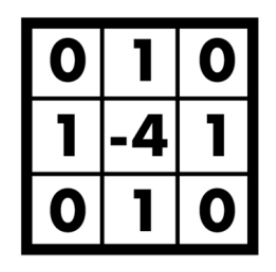
\includegraphics[width=0.1\textwidth]{figures/laplacian_kernel.png}
\caption{Laplacian kernel}
\label{fig:laplacian_kernel}
\end{figure} 




\subsubsection*{Canny Edge detector}
This edge detector is a sequence of steps:
\begin{enumerate}
	\item Smooth the image with gaussian filter
	\item Calculate gradient direction and magnitude
	\item Non-maximum suppression perpendicular to edge
	\item Threshold into \textit{strong, weak, no edge} 
	\item Connect components
\end{enumerate}


Here are the sobel kernels:
\begin{figure}[H]
\centering
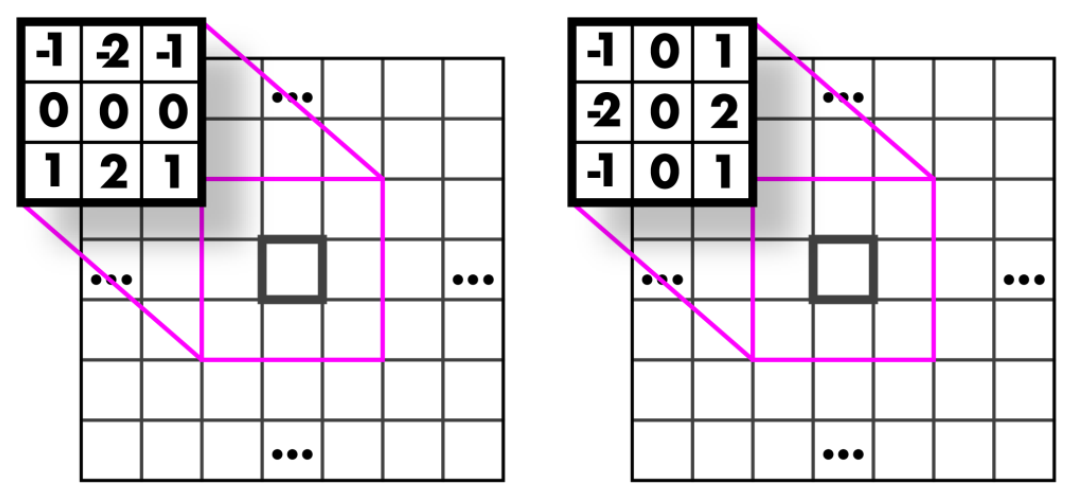
\includegraphics[width=0.5\textwidth]{figures/sobel_kernels.png}
\caption{Horizontal and vertical sobel kernels}
\label{fig:sobel_kernel}
\end{figure} 

\textbf{Compute gradients} 
Compute gradients which are perpendicular to edges, and then look in that direction, but keep only the highest pixel. The goal is to get single pixel edges and not blurry and thick lines.



\textbf{Connect components} 
This step involves connecting the classes of edges. 
\begin{itemize}
	\item Strong edges are edges!
	\item Weak edges are edges \textbf{if they connect to strong edges }
	\item 
	\item
	\item
	\item
\end{itemize}





% -----------------------------------------------------------------------------------------------------------------------
\newpage
\centering
\section{Pool}
\raggedright
\newpage
\subsection{Harris Corner, HOG, SIFT}
Features are good and still relevant. They are used in recognition, detection, image stitching and visual odometry and SLAM. They do not need training, as they are extracted with simple algorithms. 
the main components of features are:
\begin{enumerate}
	\item Detection - Detect the features, and extract their information and position.
	\item Description - The feature descriptor is what describes the feature. This should be as unique as possible.
	\item Matching - E.g. determining corresponding between two describtors in two views/images. 
\end{enumerate}

Examples of features:
\begin{itemize}
	\item Sky - Bad (little variation $ \rightarrow  $ easily mistaken to be somewhere else)
	\item Edges - mid (provide uniqueness in one direction)
	\item Corners - Best (provide positional uniqueness across entire image. Very few potential matches. )
\end{itemize}

You could compare every feature to every other feature, but this scales horibly, $ O n^{2} $\\
To get a measure of uniqueness, you could do self difference. Compute the self of the image with a template of the feature, and do template matching with distances.
\begin{equation}\label{eq:self_difference}
	\sum_{d}^{}{\sum_{x,y}^{}{(I(x,y) - I(x+dx, y+dy))^{2} }}
\end{equation}
Which computes the distance between the patch and other pixels in the kernel for the entire image. 


\subsubsection{Gradient analysis}
To analyse gradients, eigenvectors and eigenvalues can be used for analysing gradients around a pixel $ p $. 
 \begin{equation}\label{eq:dist_nearby_gradients}
	 S_w[p] = \begin{bmatrix}
		 \sum_{r}w[r](I_x[p-r])^{2} & \sum_{r}w[r]I_x[p-r] I_y[p-r] \\
	  \sum_{r}w[r]I_x[p-r] I_y[p-r] & \sum_{r}w[r](I_y[p-r])^{2}
	 \end{bmatrix}
\end{equation}
Where $ r $ is the radius from pixel  $ p $ that determines the weight of the gradients $ I_x $ and $ I_y $ round the pixel. The eigenvalues of (\ref{eq:dist_nearby_gradients}) summarize the distribution of gradients of the pixel $ p $. 
if
\begin{itemize}
	\item $ \lambda_1 $ and $ \lambda_2 $ are both small  $ \rightarrow  $ then there is no gradient.
	\item $ \lambda_1 >> \lambda_2 $ or opposite, gradient in one direction.
	\item $ \lambda_1 $ and $ \lambda_2 $ are both large, multiple gradient directions $ = $ corner
\end{itemize}

Eigenvalue computation is expensive however, therefore does the Harris Corner apporoximate the eigenvalues.


\subsubsection{Harris corner}
The algorithm:
\begin{enumerate}
	\item Calculate derivatives $ I_x $ and $ I_y $.
	\item Calculate products $ I_xI_x, I_yI_y, I_xI_y$.
	\item Compute the weighted sums based on  (\ref{eq:dist_nearby_gradients}) .
	\item Estimate response based on smallest eigenvalue.
	\item Non-maximum suppression (like Canny-edge).
\end{enumerate}
\textbf{It IS rotation invariant} $\rightarrow $ eigenvalues are the same.

\begin{figure}[H]
\centering
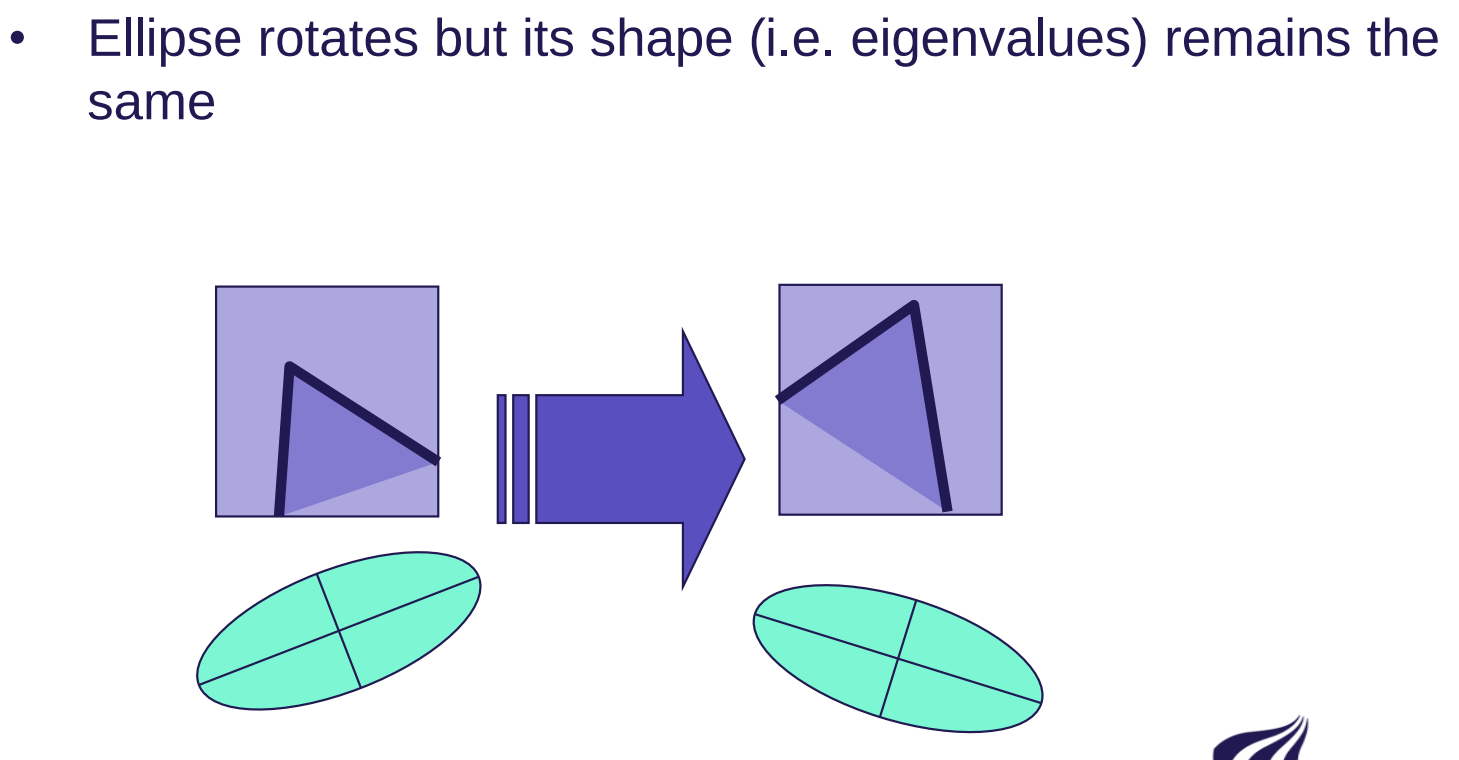
\includegraphics[width=0.5\textwidth]{figures/harris_rotation.png}
\caption{Harris corner rotation invariance}
\label{fig:harris_rot_invariance}
\end{figure} 

 \textbf{It is not Intensity invariant} $ \rightarrow $ because of fixed threshold on non maximum suppression.  \\
 \textbf{It is not Scale invariant} $ \rightarrow $ The eigenvalues scale with the window size used for gradient computation, and because the gradients magnitude affects the eigenvalues. 


\subsubsection{HOG - Histogram of Oriented Gradients}
Objects can be described by the distribution of local intensity gradients. Originally proposed as a pedestrian detector. It is computed in windows which are slid across the entire image. 
\begin{enumerate}
	\item Normalize color \\
		Make every color between 0 and 1
	\item Compute gradients\\
		Use sobel kernels $ \begin{bmatrix} -1 & 0 & 1  \end{bmatrix}  $ and $ \begin{bmatrix} -1 & 0 & 1  \end{bmatrix}^{T}   $
	\item Weighted vote into spatial orientation cells
	\item Contrast normalize over overlapping spatial blocks
		We make blocks that span multiple cells. Compute the L2-norm and divide each gradient with that. 
	\item Collect HOG's over detection window\\
		Concatenate all gradient bins into one long feature vector for a single window. 
	\item \textit{Run linear SVM classifier} \\
		Could be used to classify e.g. if it is a person.
\end{enumerate}
As seen in Figure (\ref{fig:HOG_features}), the longer arrows in a cell (usually $ 8 \times 8 $) means more predominant edge in that particular direction. Then we assemble the gradients in histograms with angle along the horizontal axis and number of edges at that angle along the vertical axis.
\begin{figure}[H]
\centering
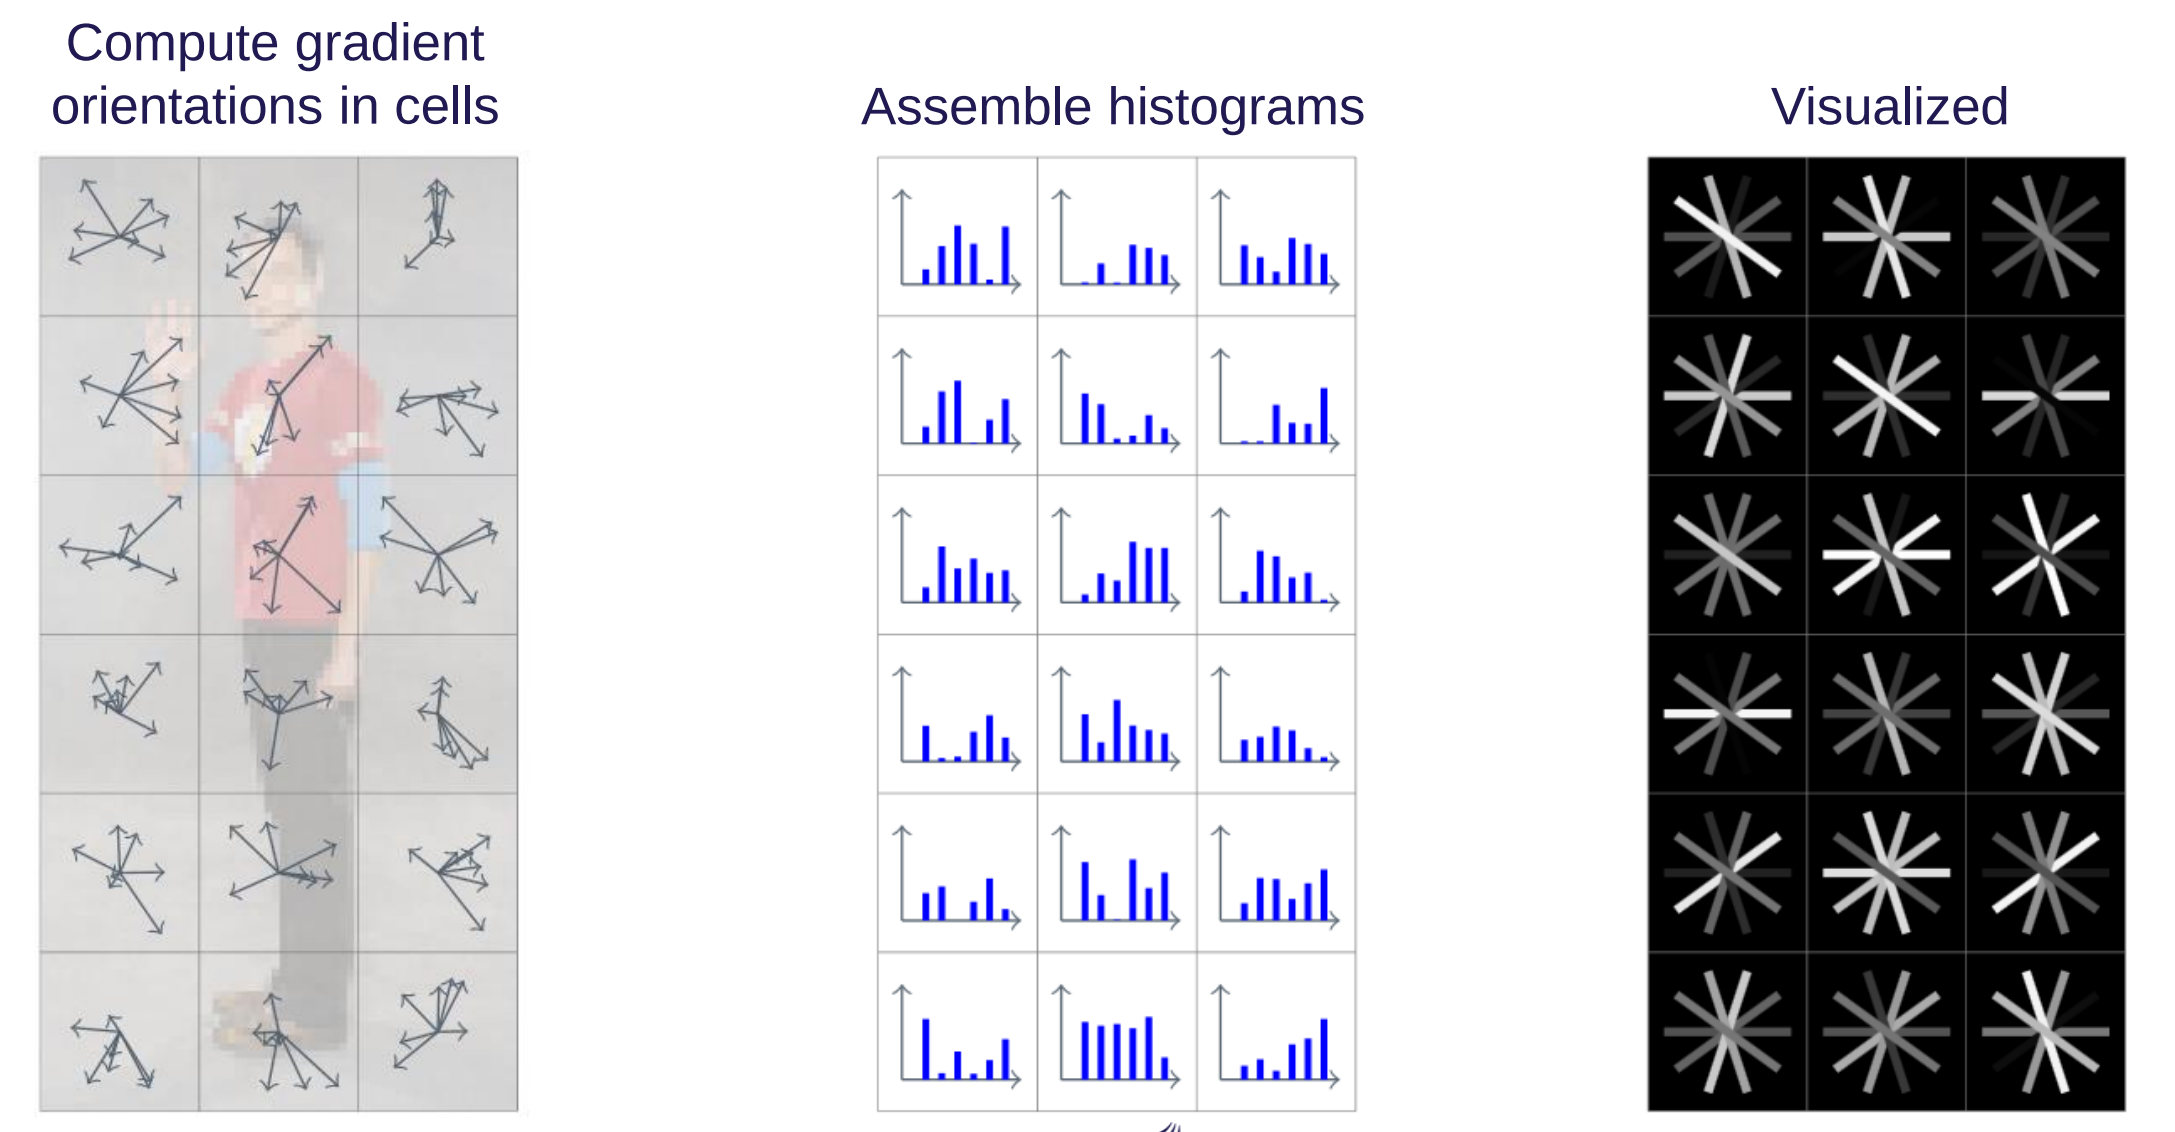
\includegraphics[width=\textwidth]{figures/HOG.png}
\caption{HOG features}
\label{fig:HOG_features}
\end{figure} 

\textbf{Lighting invariant} \\
\textbf{Scale invariant} \\
\textbf{Not rotation invariant} 

\subsubsection{SIFT - Scale Invariant Feature Transform}
We try to compute scale invariant features.

\begin{itemize}
	\item Scale-space extrema detection
	\item Keypoint localisation
	\item Orientation assignment
	\item Keypoint descriptor
\end{itemize}

SIFT focusses on both \textit{detection} and \textit{description}  


The image is asigned different scales. These are assigned into what is know as \textit{octaves}. In each octave we convolve gaussians with different $ \sigma $-values, which affects the degree of blurring. Two adjecent gaussians are subtracted, which gives the  \textit{DoG}. This results in images that containes edges, and works like a low and high pass filter depending on the $ \sigma $-value. For large $ \sigma $-values, the large changes (low frequencies) are extracted, and vice versa. 
\begin{figure}[H]
\centering
\includegraphics[width=0.5\textwidth]{figures/SIFT_extrema_detection.png}
\caption{SIFT extrema detection}
\label{fig:sift_extrema_detection}
\end{figure} 

In this step we determine if the keypoint is an extrama, by considering the scale above and the scale below. If these are all above or below the pixel, then we have an extrema. 
\begin{figure}[H]
\centering
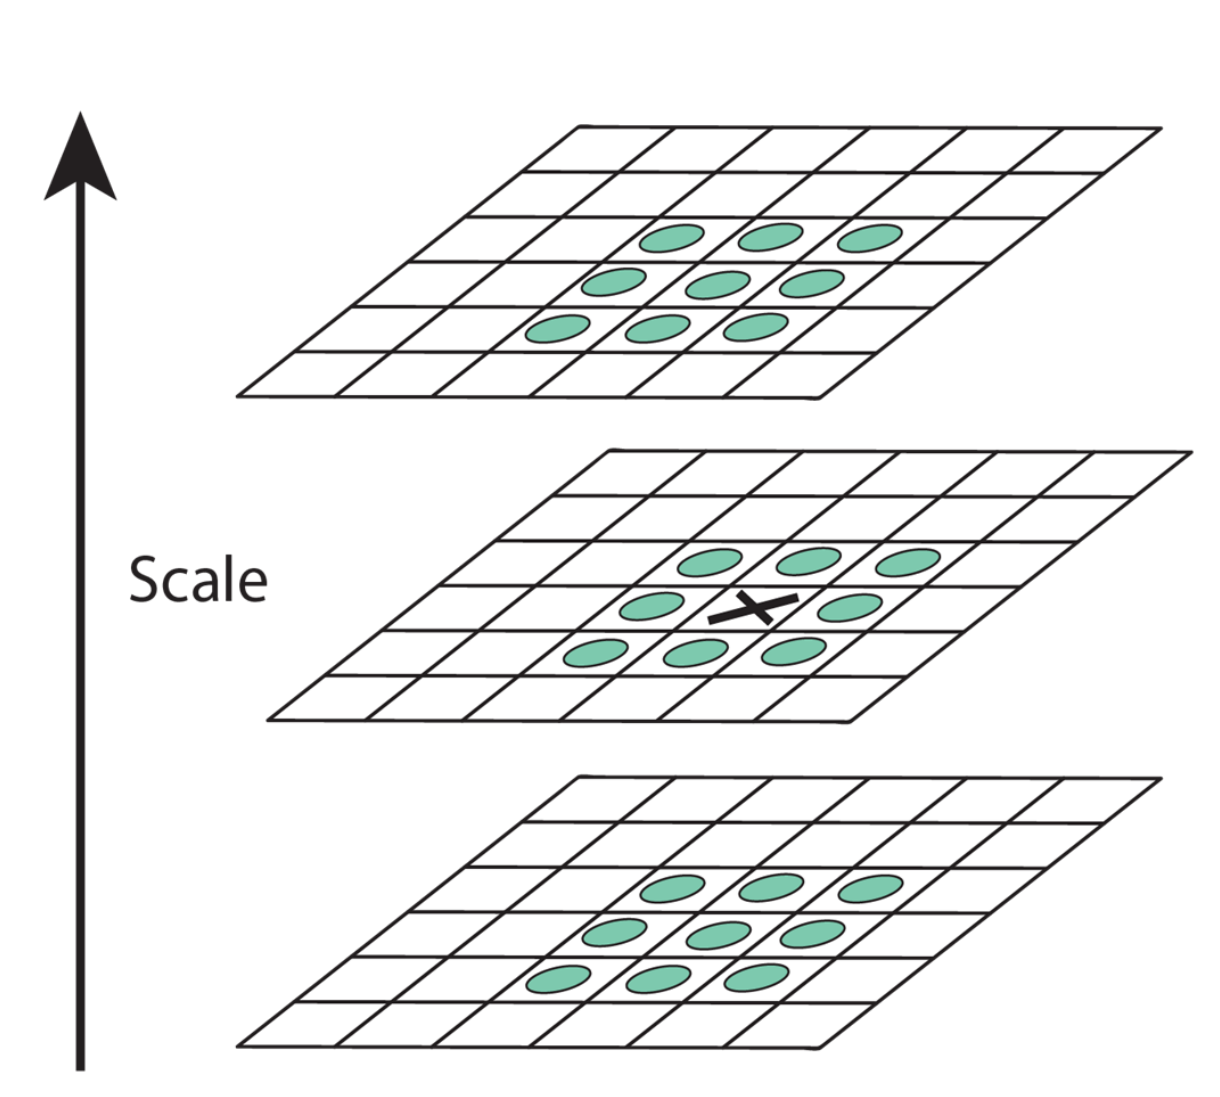
\includegraphics[width=0.5\textwidth]{figures/Local_extrema_location.png}
\caption{The local extrema location across adjecent scales. }
\label{fig:local_extrema_location}
\end{figure} 

In this step, we assign orientation based on the patches in the image. We assign 36 orientation histogram bins, and these are weighted by the gradient magnitude and gaussian-weighted distance from the keypoint. We assign the most dominant direction as the orientation of the keypoint, and we also assign keypoint descriptors for bins above $ 80\% $.
\begin{figure}[H]
\centering
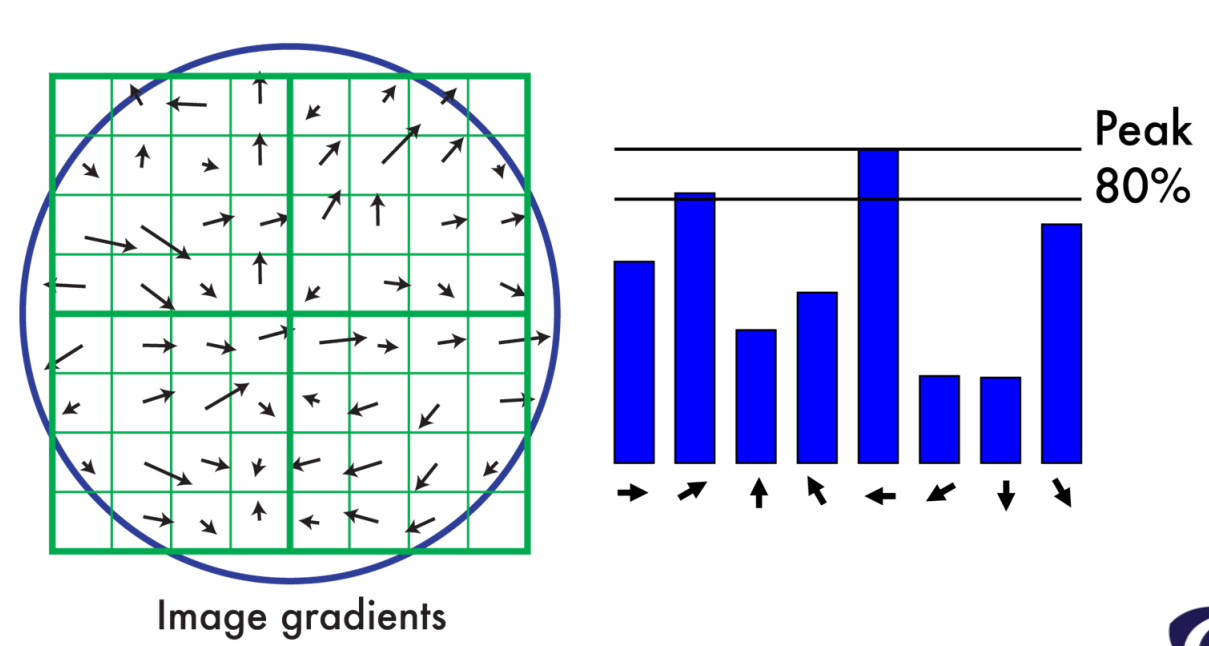
\includegraphics[width=0.8\textwidth]{figures/SIFT_patch_orientation.png}
\caption{Patch orientation for SIFT keypoints}
\label{fig:Patch_orientation}
\end{figure} 


We rotate the the feature relative to the keypoint orientation.
This makes it rotation invariant. \\
The feature descriptor must be illumination invariant as well, this is done by normalizing the feature descriptor vector to unit length, thresholding the descriptor above $ 0.2 $, so we disregard any light intensities below  $ 0.2 $ and we normalize once again. 

\begin{figure}[H]
\centering
\includegraphics[width=\textwidth]{figures/SIFT_result.png}
\caption{The SIFT algorithm visualized}
\label{fig:SIFT_result}
\end{figure} 

Problems:
\begin{itemize}
	\item Computationally heavy $ \rightarrow $ slow in some scenarios
\end{itemize}
Alternatives
\begin{itemize}
	\item SURF
	\item ORB (fast for realtime.)
\end{itemize}



% -----------------------------------------------------------------------------------------------------------------------
\newpage
\subsection{Linear regression, RANSAC}


\subsubsection{RANSAC - RANdom Sample Consensus}
E.g. a way of matching two images, where we consider inliers and outliers. If there is enough inliers, we have can make an image transformation, because there may be a lot of feature matches agree on some image transformation, then we may use this image transformation.

\textbf{Algorithm:} 
\begin{enumerate}
	\item Select a random subset of the of original data
	\item A model is fitted to this subset (e.g. Linear regression)
	\item Determine how many points fit within a predefined tolerance (inliers vs outliers)
	\item If the fraction of the total number of inliers relative to the number of data points in the subset are above some threshold, we refit the model to the set of inliers, and then we terminate. 
	\item Otherwise repeat step $1-4$ (max N times)
\end{enumerate}

We select e.g. 2 points and fit a model to these two points $ \rightarrow $ A single line between the two points. Then we compute the number of inliers of that model based on the predefined tolerance threshold. If we see enough inliers, then terminate. 

\begin{figure}[H]
\centering
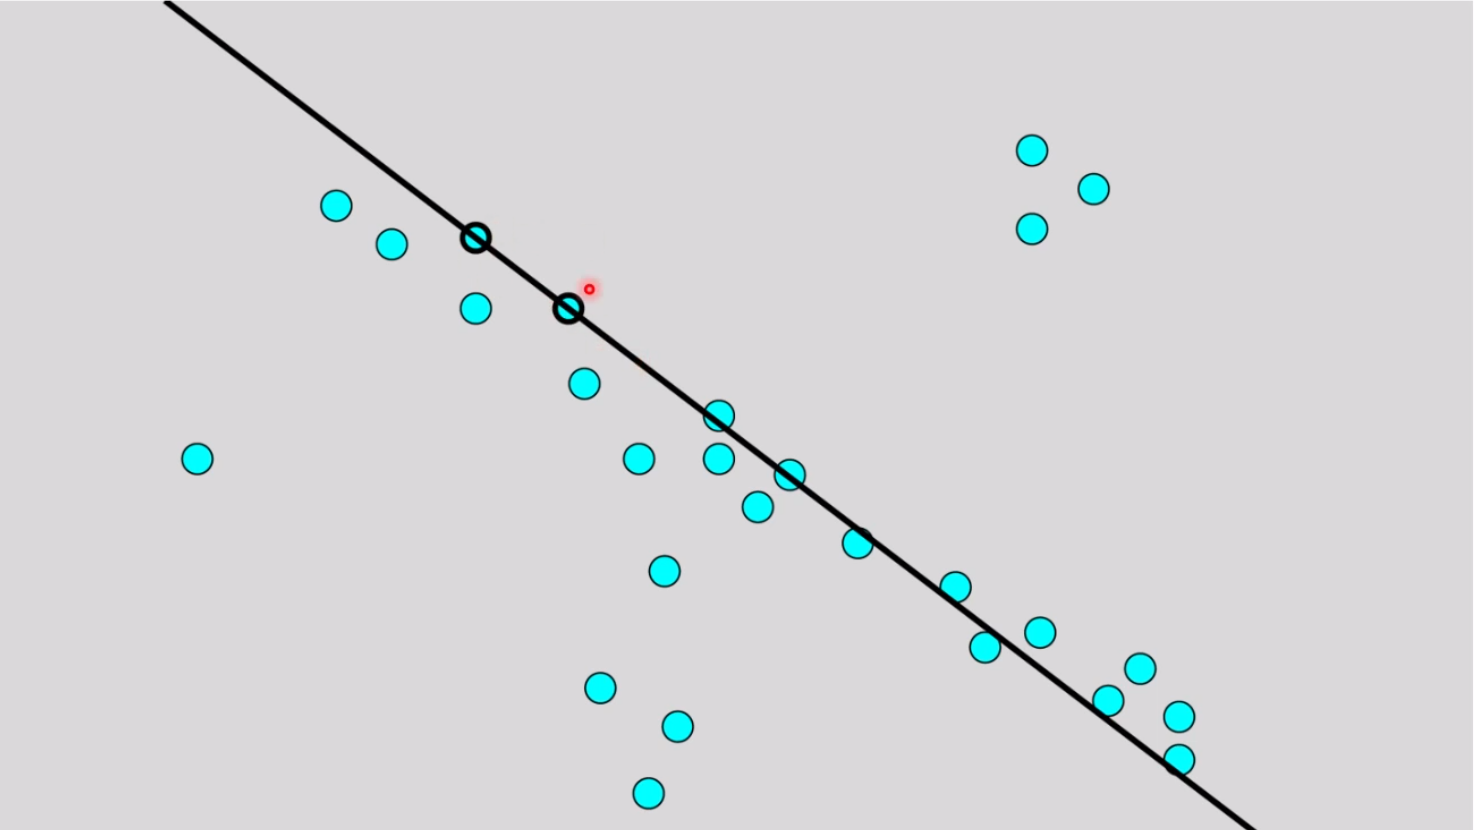
\includegraphics[width=0.8\textwidth]{figures/RANSAC.png}
\caption{Illustration of the RANSAC algorithm}
\label{fig:RANSAC}
\end{figure} 

It has a lot of different hyper parameters.
\begin{itemize}
	\item $ t $ threshold from the model $ \rightarrow $ quite small
	\item $ n $ number of points to fit the model $ \rightarrow $ 2 for a line 
	\item $ k $ is the number of itterations $ \rightarrow $ can be high
	\item $ d $ good fit cutoff. How many inliers are considered engough to consider a good model.
\end{itemize}

\textbf{Note may need to elaborate on linear regression} 

% -----------------------------------------------------------------------------------------------------------------------
\newpage
\subsection{PCA-LDA - Principal Component Analysis, Linear Discriminant Analysis}
Dimensionality reduction. We have some featurevector with a high dimensionality of features, and the goal is to reduce the dimensionality of the feature vector, while still preserving the variance of the data, which says something about the information of the data. 

\subsubsection{PCA}
\textbf{Algorithm} 
\begin{itemize}
	\item \textbf{Standardize} the data (compute mean and subtract, to center around 0)
	\item Compute \textbf{covariance}  matrix of standardized data. 
	\item Compute \textbf{eigenvectors} and corresponding \textbf{eigenvalues}  of the covariance matrix
		\begin{figure}[H]
		\centering
		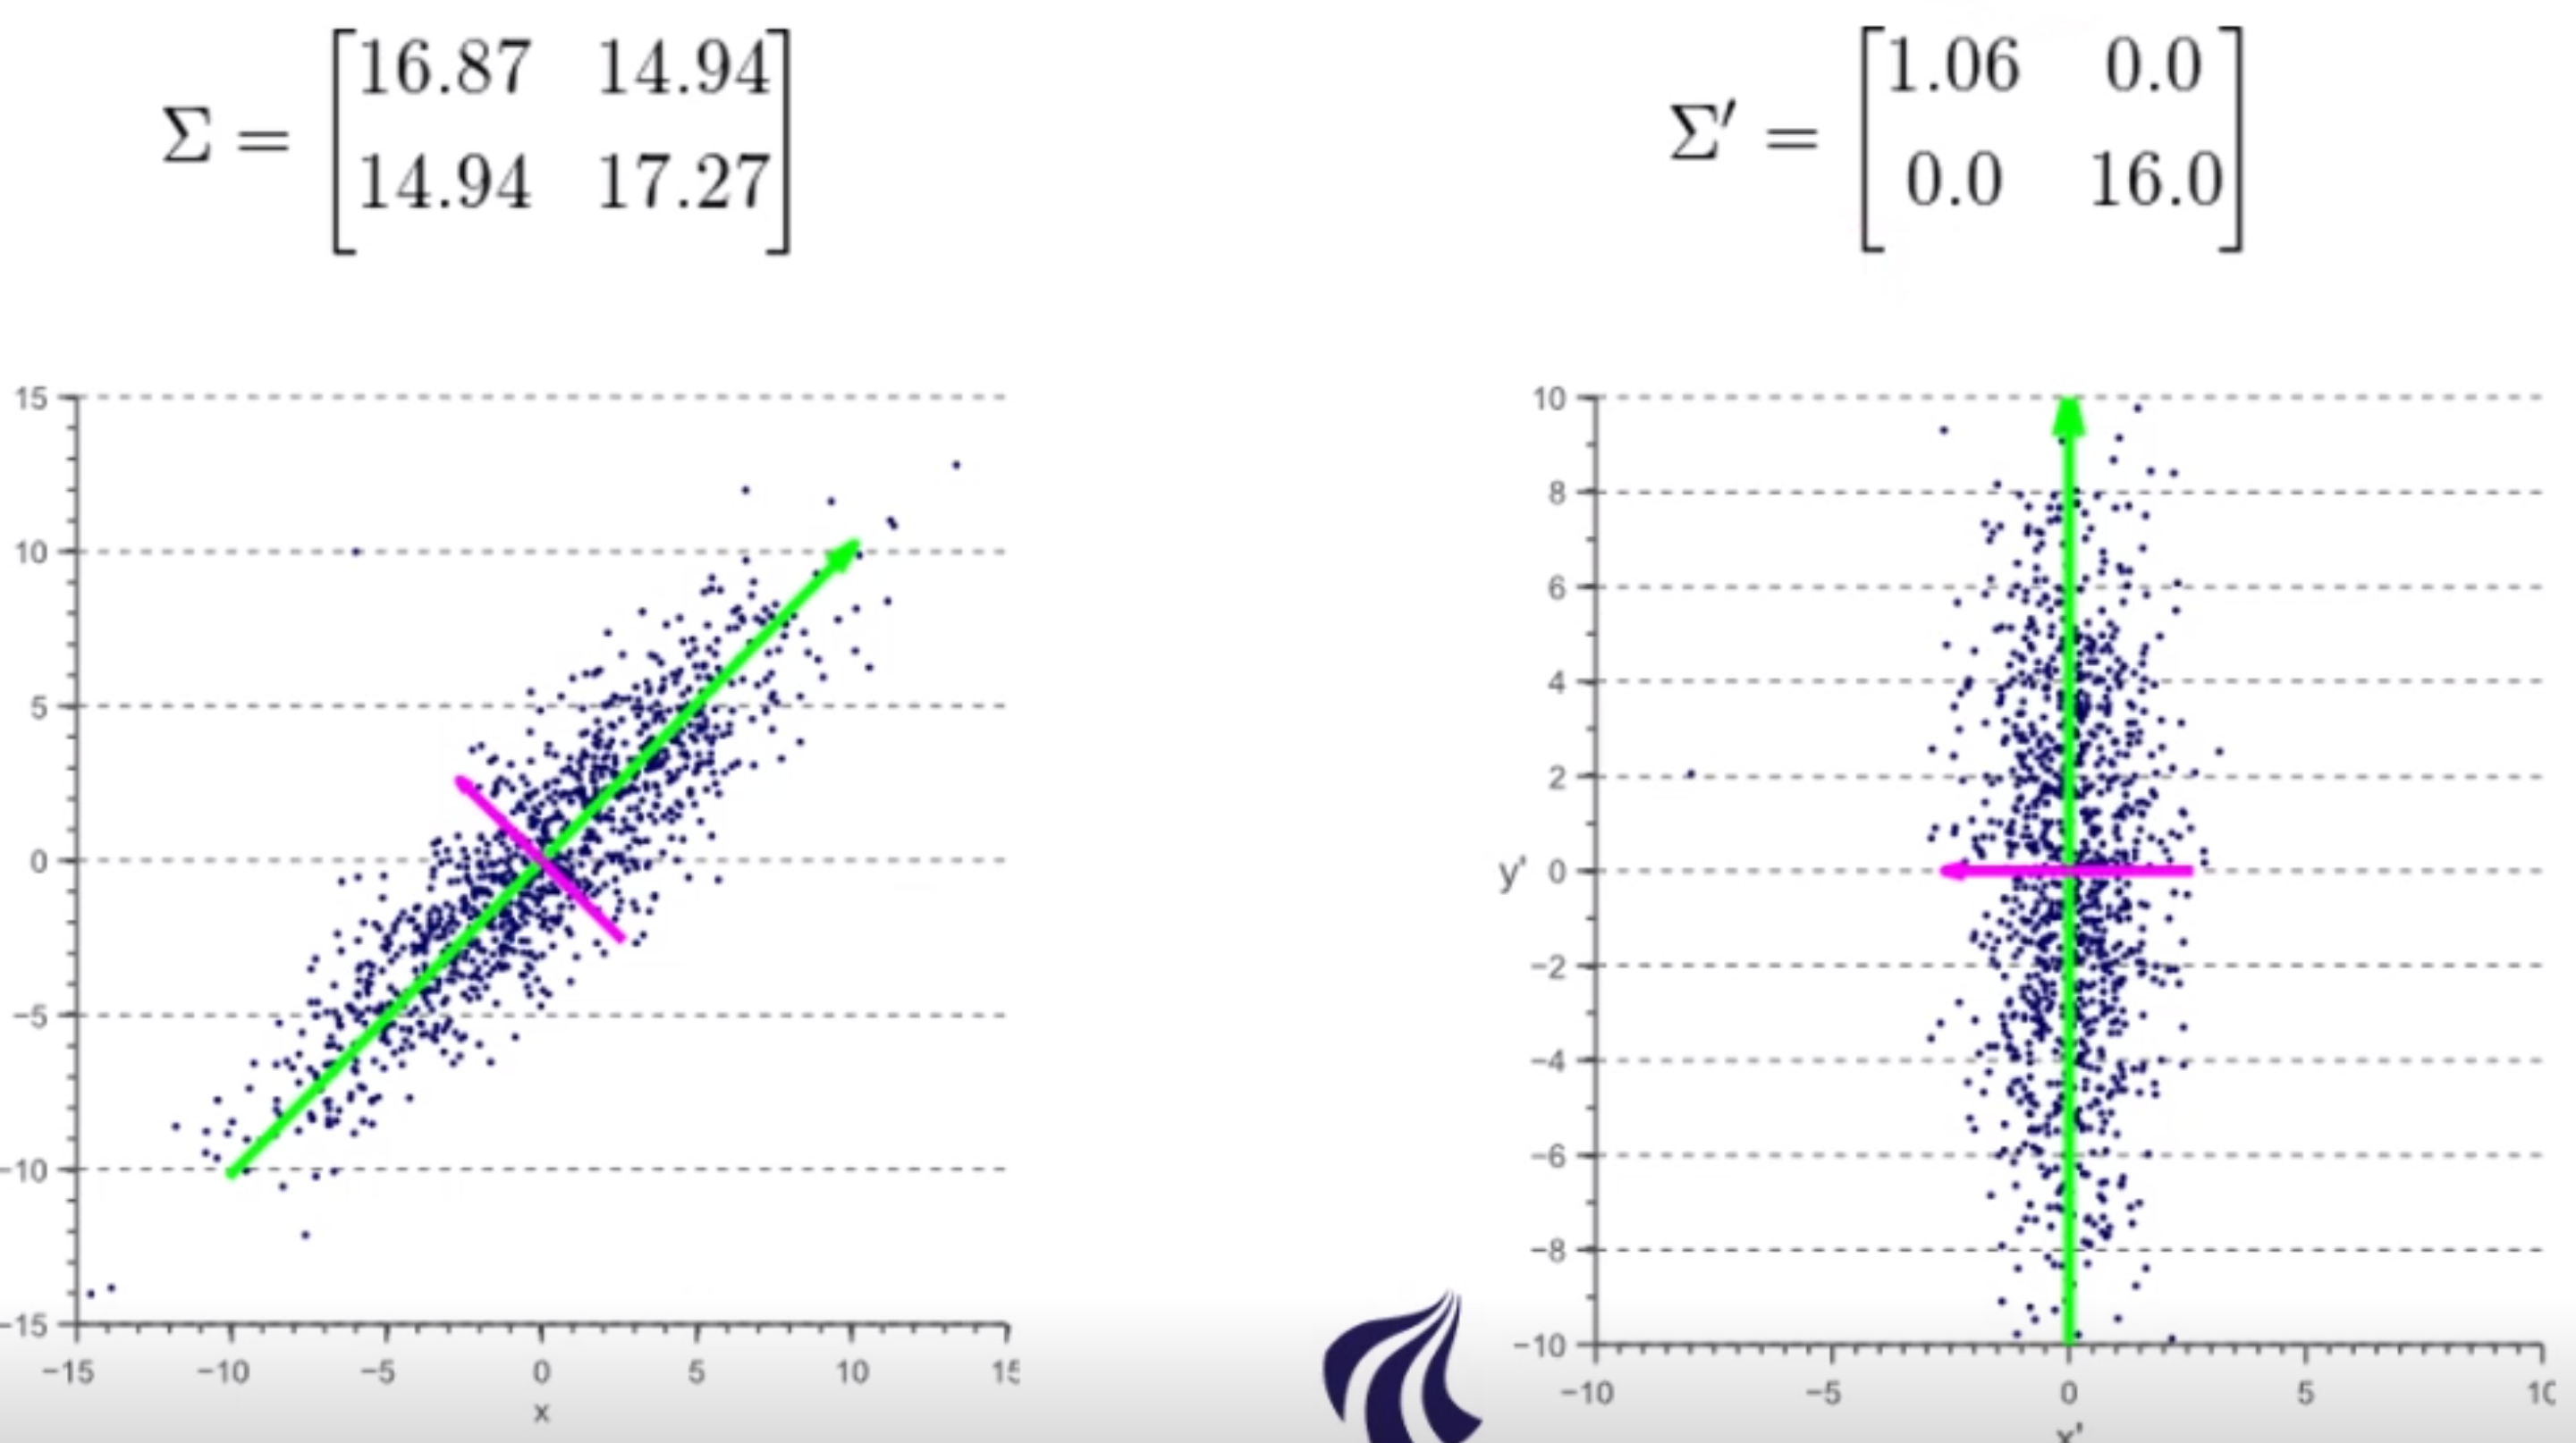
\includegraphics[width=0.5\textwidth]{figures/PCA_cov.png}
		\caption{Covariance computation and Transformation.}
		\label{fig:pca_cov}
		\end{figure} 
		
	\item \textbf{Transform}  the data using the $ n $ most significant variances.
		\begin{figure}[H]
		\centering
		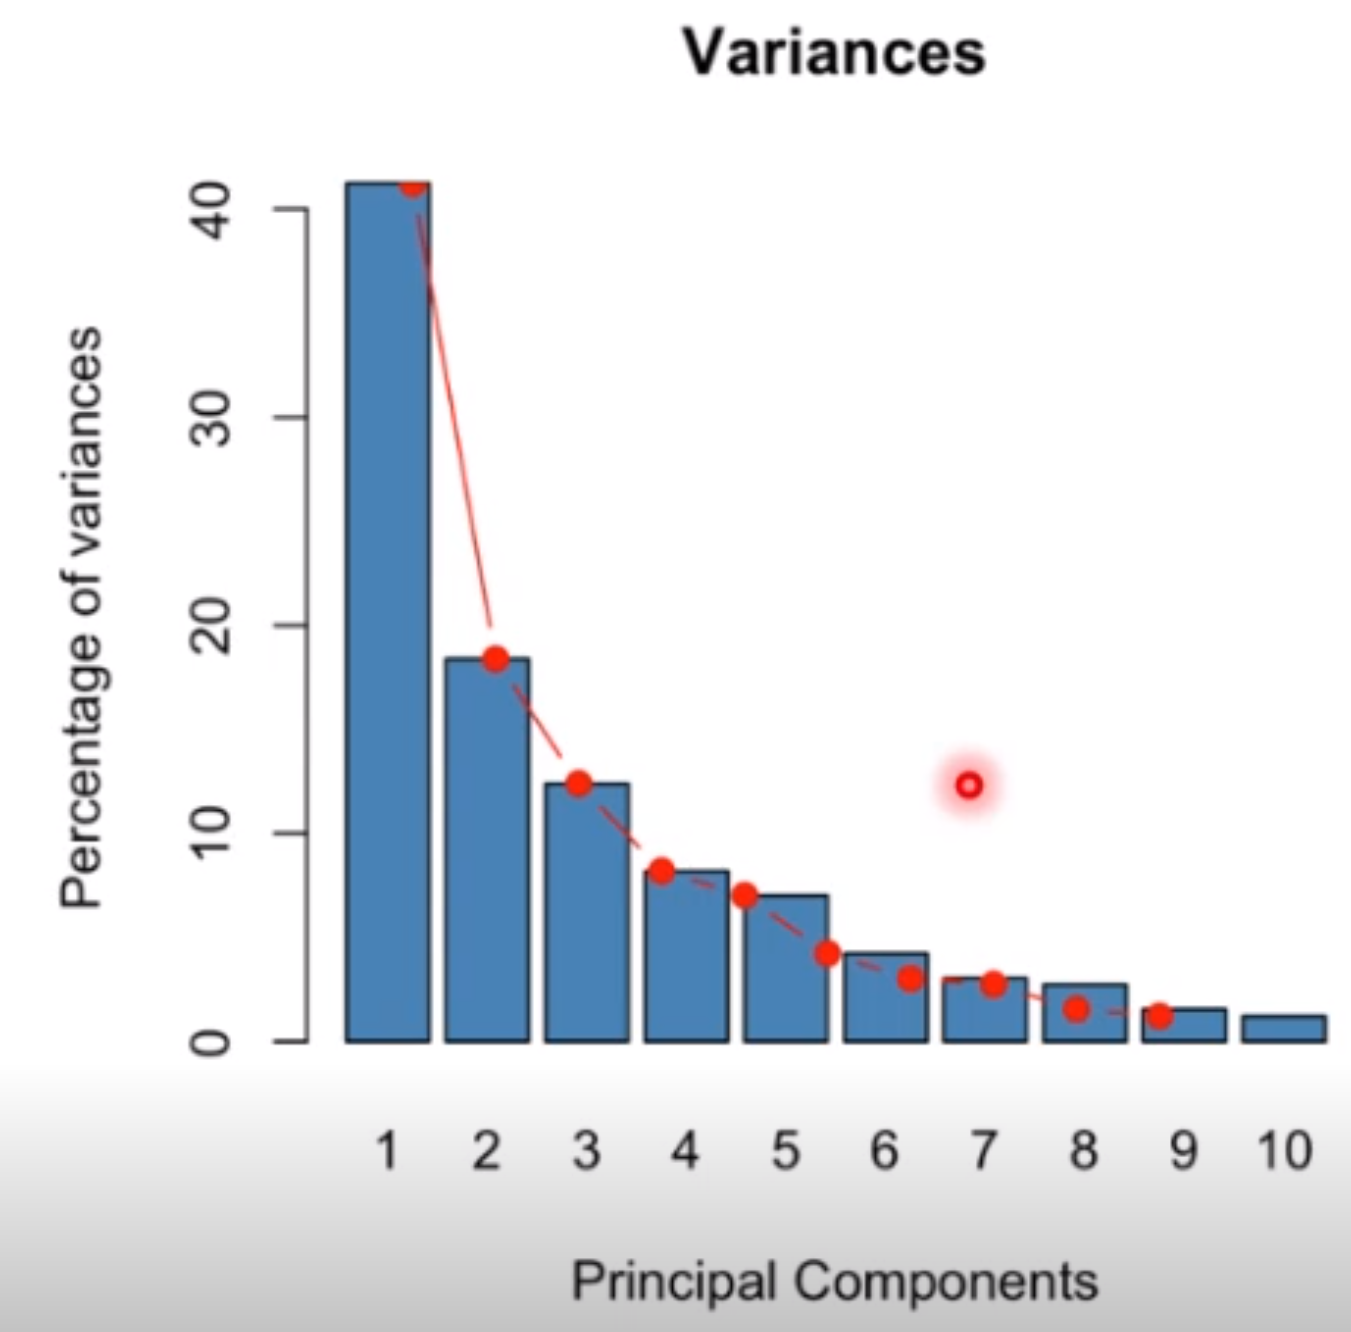
\includegraphics[width=0.5\textwidth]{figures/PCA_variance_order.png}
		\caption{PCA percentage of variances}
		\label{fig:pca_variances}
		\end{figure} 
\end{itemize}

\textbf{Problems:} 
\begin{itemize}
	\item Unsupervised $ \rightarrow $ no knowledge of the classes of the data
\end{itemize}


\subsubsection{LDA}
Uses labelled data. Finds the direction that best discriminates between classes. I.e. Best way of splitting the classes up for easy classification. \\
Also known as Fishers Linear Discriminant. (small difference in assumptions)

\textbf{Based on 2 different computations} 
\begin{itemize}
	\item Within-class scatter:
	\begin{equation}\label{eq:within_class_scatter}
		S_w = \sum_{i=1}^{c}{\sum_{x \in C_i}^{}{(x-m_i)(x-m_i)^{T} }}
	\end{equation}
	\item Between-class scatter:
	\begin{equation}\label{eq:between_class_scatter}
	S_B = \sum_{i=1}^{c}{n_i(m_i - m)(m_i - m)^{T} }
	\end{equation}
\end{itemize}
Where $ x $ is a sample of class $ i $, $ c $ is the total number of classes and $ m_i $ is the sample mean of class $ i $. $ n_i $ is the number of samples in class $ i $, and $ m $ is the total sample mean. \\
So in (\ref{eq:within_class_scatter}) the difference between the sample and the mean of that class is comuted and summed. Basicly the same as computing variance. \\ 
In (\ref{eq:between_class_scatter}) the computed mean of each class vs the total mean is computed. This tells us the magnitude of the variance of all the classes, i.e. how far appart these classes are. 

We then want to find the transformation that maximises the ration between the within-class scatter and between class scatter. 
\begin{equation}
	W_{opt} = argmax_w  \frac{|W^{T} S_B W|}{|W^{T} S_W W|} 
\end{equation}


% -----------------------------------------------------------------------------------------------------------------------
\newpage
\subsection{Background subtraction, image differencing}

\subsubsection{Background Subtraction}
Video is a function $ f(x,y,t) $. Use a time dimension to segment the video frames. \\
\textbf{Segmentation} $ \rightarrow $  seperation of forground and background. (binary images.)
You can do background subtraction in videoes. \\
\textbf{Basic algorithm} 
\begin{enumerate}
	\item Capture image containing the stable background.
	\item Capture a new frame sometime in the future and compare them.
	\item Subtract frame from background (use absolute difference to avoid negative values.)
	\item Threshold difference (there may be small differences due to noise)
	\item Delete the noise (use median filter, bigger kernels remove larger spots, or use Morphology(opening/closing))
\end{enumerate}
\begin{figure}[H]
\centering
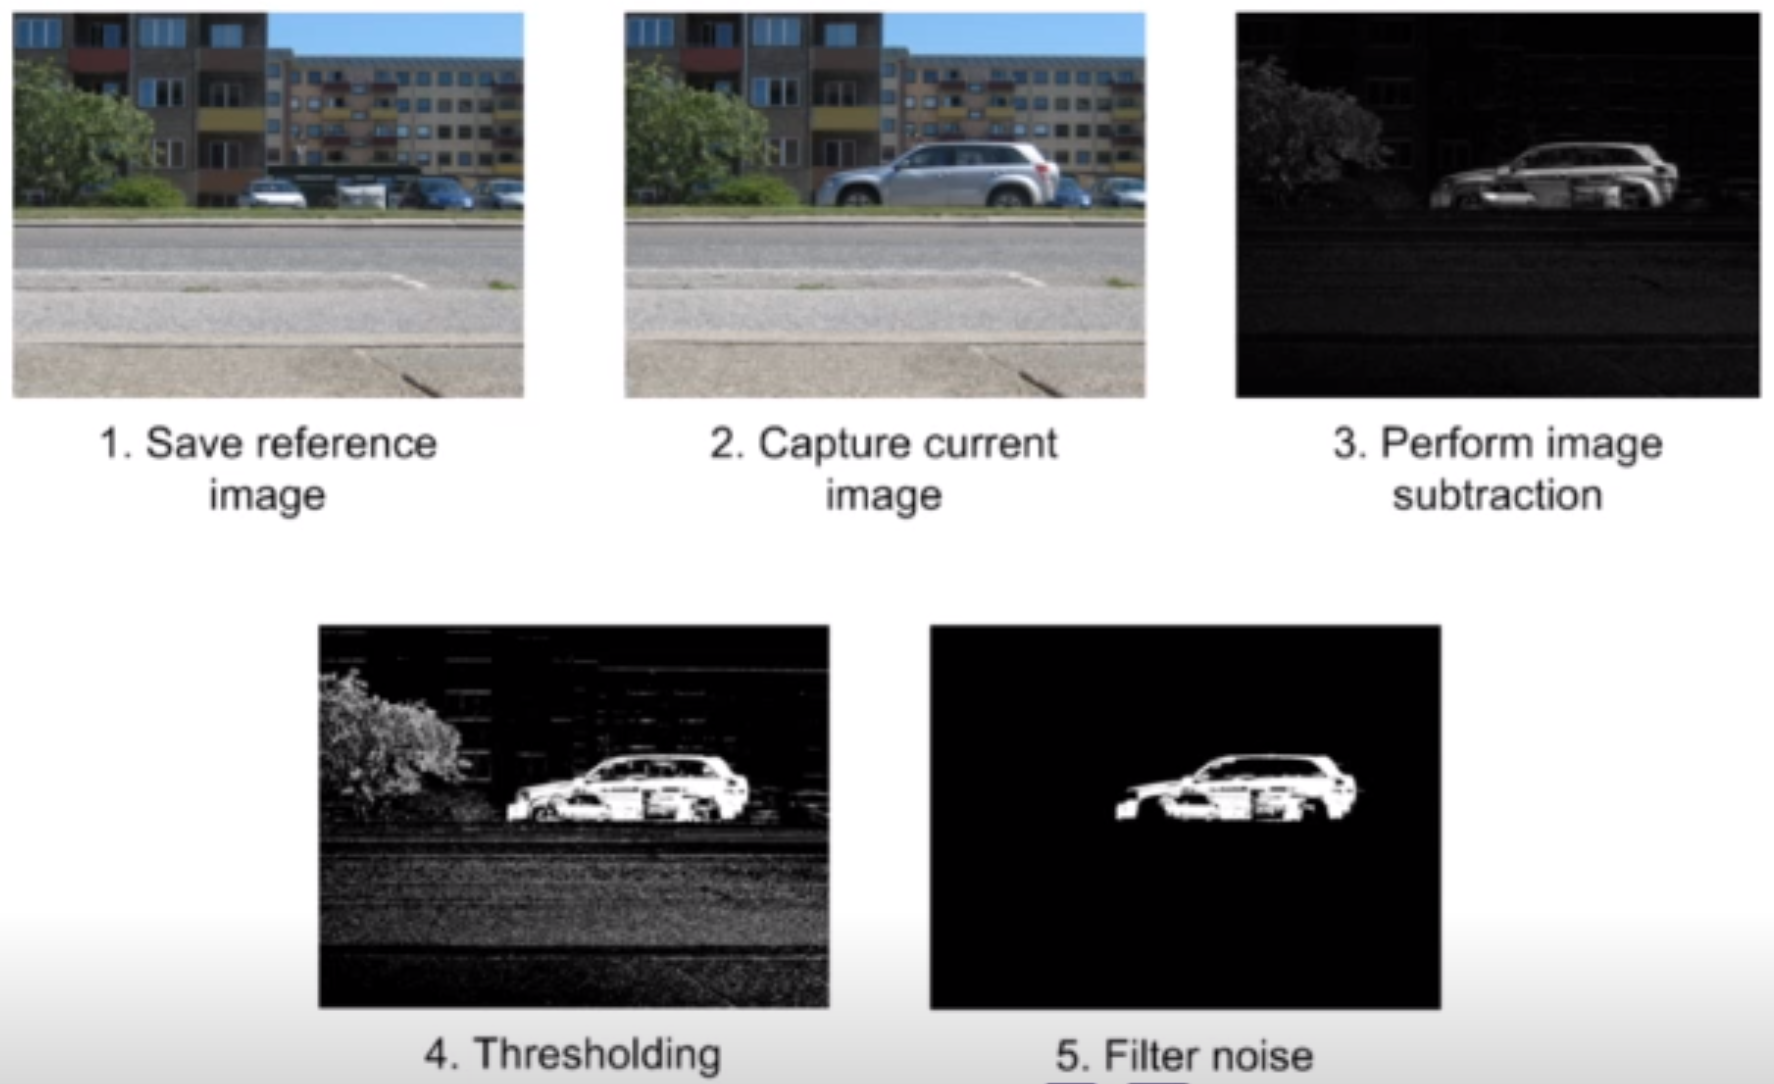
\includegraphics[width=0.9\textwidth]{figures/Background_subtraction_basic.png}
\caption{Basic background subtraction algorithm}
\label{fig:basic_background_subtraction}
\end{figure} 

Requires \textbf{completely static background} 


\textbf{Advanced background subtraction} 
Almost static background (noise, light changes, small motion (wind blowing in trees))\\
Compute \textbf{average background image}.
\begin{equation}
B(x,y) = \sum_{i=1}^{N}{\frac{I_i(x,y)}{N} }
\end{equation}
where $ I_i $ is the $ i $'th image and $ N $ is the total number of images. \\
Threshold should be different for different pixels in the image, as they may vary in variance. \\
We can learn these thresholds:

\vspace{5pt}
Gaussian models (mean and variance) for each pixel.
\begin{equation}
TH = K \cdot \sigma(x,y)
\end{equation}


 You could also\textbf{ Update the reference image.} 

 

\subsubsection{Image differencing}
Very dynamic scenes $ \rightarrow $ Background cannot be learned.\\
Use any previous image as the reference image. depending on how close to the captured frame you want. \\
Subract them and look at what moved. \\
You can look at two different reference frames and \textbf{AND} them together.
\begin{figure}[H]
\centering
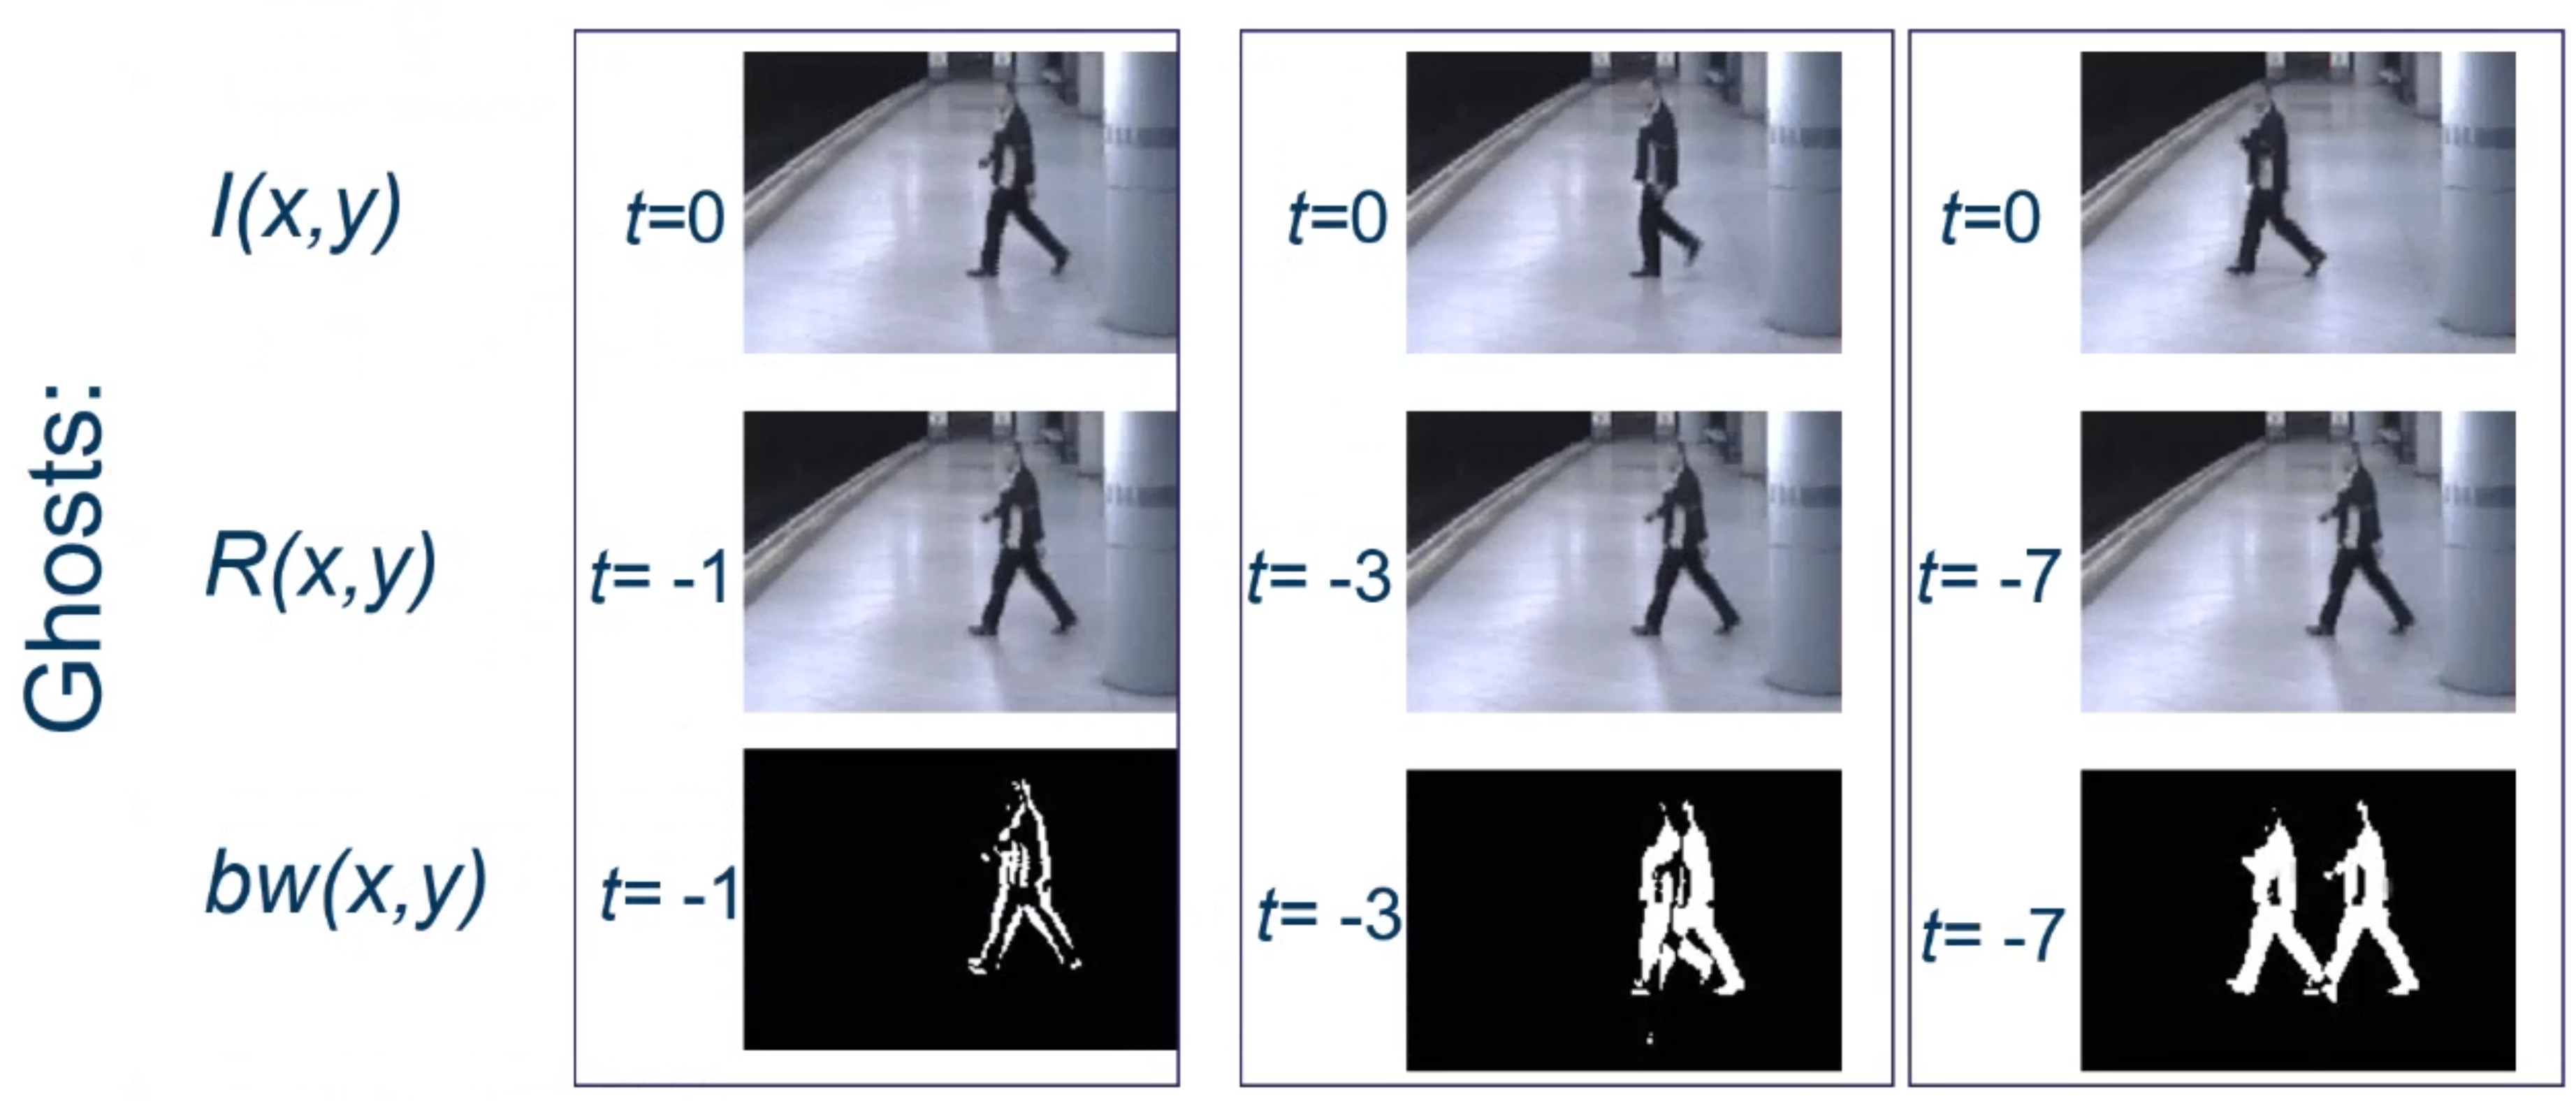
\includegraphics[width=0.9\textwidth]{figures/Image_differencing.png}
\caption{Image differencing at 1. 3 and 7 frame differences.}
\label{fig:image_differencing}
\end{figure} 

Note that if the time difference is great, it may be difficult to do data association between two BLOB's. This is considered \textbf{Ghosting} 

\begin{figure}[H]
\centering
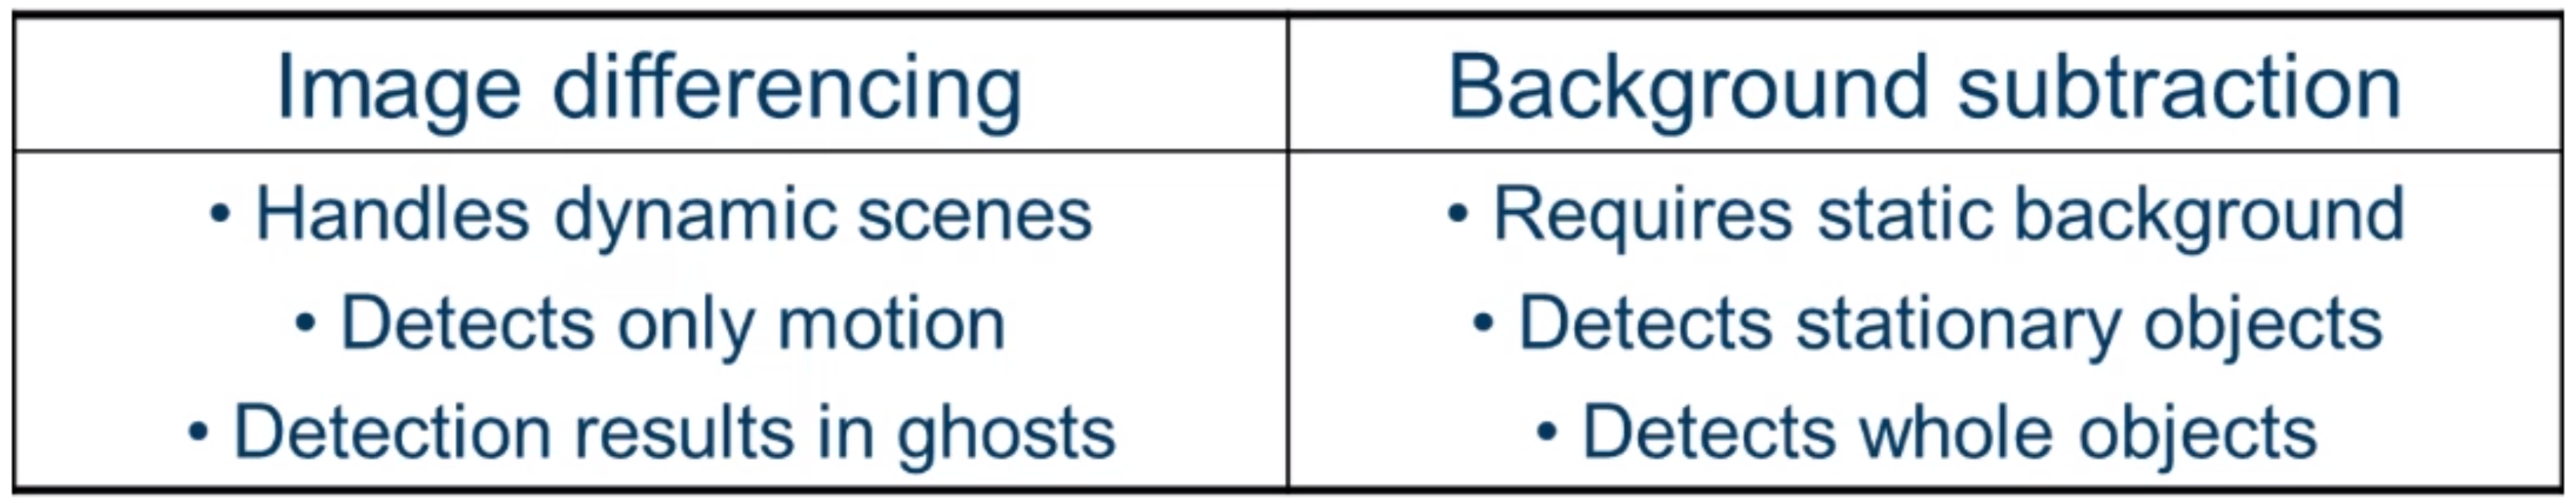
\includegraphics[width=0.8\textwidth]{figures/Background_image_differencing_comparison_table.png}
\caption{Background subtraction and image differencing comparison.}
\label{fig:Background_Imagedifferincing_comparrison}
\end{figure} 

% ----------------------------------------------------------------------------------------------------------------------
\newpage
\subsection{Optical Flow}
Motion analysis.\\
Can detect both object motion and camera motion. \\
Can be used in \textbf{Visual Odometry}.\\
We can detect type of motion by looking at the difference vectors and their magnitudes. 
\begin{itemize}
	\item Rotation
	\item Horizontal translation
	\item Larger vectors appear to move faster, or are closer to the camera. 
\end{itemize}
We can \textbf{not} just use \textbf{feature matching} because:
\begin{itemize}
	\item Sparse (needs good features)
	\item Feature alignment may not be exact. 
	\item Low accuracy for entire image. 
	\item Assumes that everything is moving with the same transformation!
\end{itemize}

\subsubsection{Lucas-Kanade Algorithm}
Based on the idea that when the object is moving in one direction, it is the same as moving the observed pixel in the opposite direction.
\begin{equation}
f(p-\Delta p, t) = f(p, t+ \Delta t)
\end{equation}
where $ p = \begin{bmatrix}
x \\
y
\end{bmatrix} $ is the observation point. $ t $ is the first image and $ t + \Delta t $ is the second image. \\
Approximate the model with taylor expansion and do some deriviation. 
\begin{equation} \label{eq:approximate_linearized_model}
	-d x \cdot  u - d y \cdot v \approx I_t[x,y] - I_{t+\Delta t}[x,y]
\end{equation}
where $ u = \Delta x$ and $ v = \Delta y $ and  $ I_t $ is the image at time $ t $
Solve for $ u $ and $ v $. $ \rightarrow $ 1 equation, 2 unknowns.\\
Therfore we look at the pixels in the \textbf{neighborhood}  $ \rightarrow $  We assume that the pixels in the neighborhood \textbf{move together} 

We express the (\ref{eq:approximate_linearized_model})  for all neighbors, and concatenate them into vectors. 

let 
\begin{align}
S &= \begin{bmatrix}
dx_1 &dy_1  \\
dx_2 &dy_2 \\ 
\vdots & \vdots \\
dx_9 &dy_9 \\ 
\end{bmatrix}\\
	\Delta p &= \begin{bmatrix}
u \\
v
\end{bmatrix}\\
T &= \begin{bmatrix}
	I_t[x_1,y_1] - I_{t+\Delta t}[x_1,y_1] \\
	I_t[x_2,y_2] - I_{t+\Delta t}[x_2,y_2] \\
	\vdots \\
	I_t[x_9,y_9] - I_{t+\Delta t}[x_9,y_9] \\
\end{bmatrix} 
\end{align}

Then the solution expression is given as:
\begin{equation}
	S \Delta p = T
\end{equation}
Which is solved with least squares giving:

\begin{equation}
	\Delta p = (S^{T} S)^{-1} S^{T} T
\end{equation}

$ S^{T} S $ must be invertible.  $ \rightarrow $ Not invertible when there is no structure around $ x $ and  $ y $. E.g. if the middle of the sky is selected.

Good  selections are corners.

\vspace{5pt}

\textbf{Problems:} 
\begin{itemize}
	\item Not lighting invariant
	\item Large movement $ \rightarrow $ Requires high framerate 
	\item Needs good feature.
	\item Appature problem
\end{itemize}
\textbf{Appature problem} 
Because of looking only in the neighborhood, it may not be possible to see the actual motion.

\begin{figure}[H]
\centering
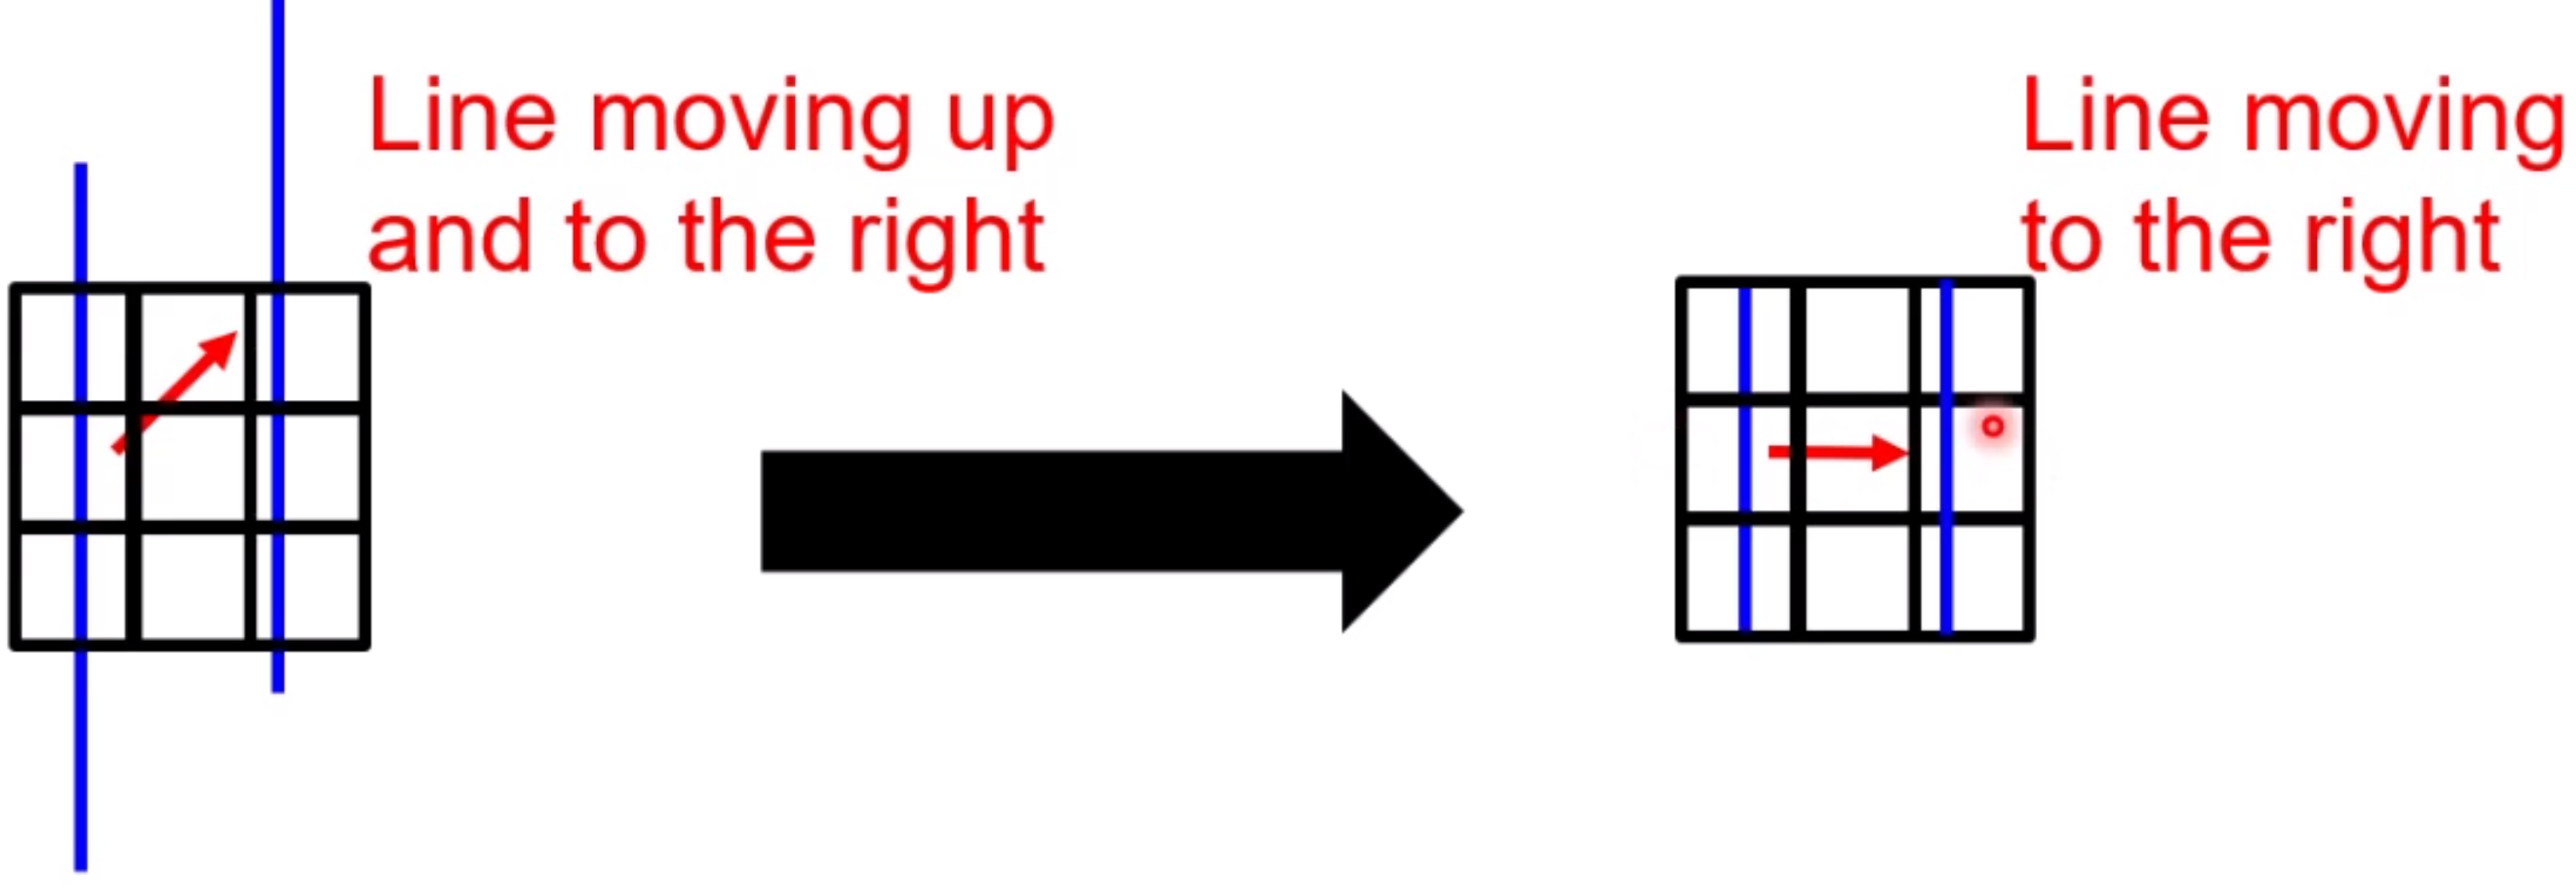
\includegraphics[width=0.8\textwidth]{figures/Appature_problem_LKA.png}
\caption{Appature problem}
\label{fig:appature_problem}
\end{figure} 

Same with the \textbf{barber pole illusion}.

% ----------------------------------------------------------------------------------------------------------------------
\newpage
\subsection{Tracking - Kalman filter, mean shift}
Using temporal information in object tracking.

One way is doing:\\
\textbf{Predict $ \rightarrow $ Match $ \rightarrow $ Update} 
This can take in no linear motion, or 1'st order linear motion $ \rightarrow $ velocity to predict next position. Or lastly 2'nd order linear motion $ \rightarrow $ Acceleration, and predicted acceleration at next time step.

\begin{itemize}
	\item 0 order linear motion $ \rightarrow $ same position
	\item 1'st order linear motion $ \rightarrow $ use velocity to predict next position
	\item 2'nd order linear motion $ \rightarrow $ Use acceleration to predict next position.
\end{itemize}

The matching state is using a \textbf{ROI} dependent on uncertainty of where the next position is. We can \textbf{scale the ROI with uncertainty $ \alpha  $} 
\begin{equation}
radius(t+1) = \alpha \cdot (p(t) - p(t) ) + (1- \alpha ) \cdot radius(t)
\end{equation}


Can track based on \textbf{appearance} or \textbf{motion model} 

\subsubsection{Kalman filter}
Set up a state vector containing fx:
\begin{itemize}
	\item Position
	\item Velocity
	\item Acceleration
	\item Size
	\item Shape
	\item Colour
	\item $ \vdots $
\end{itemize}

\textbf{Prediction} 
\begin{enumerate}
	\item Predicting the next state: \begin{equation} \hat{x}_k = A \hat{x}_{k-1} + B u_k + w_k \end{equation}
	\item Error covariance propagation. \begin{equation} P_k = A P_{k-1} A^{T} + Q \end{equation}
\end{enumerate}



\textbf{Measurement} 
\begin{equation}
	z_k = H x_k + v_k
\end{equation}
where $ H $ is the observation model $ \rightarrow $ maps from state-space to measurement space\\
$ w_k $ and  $ v_k $ are random gaussian noise random variables.

\begin{enumerate}
	\item Compute kalman gain:
		\begin{equation}
			K_k = P_k H^{T}(H P_k H^{T} + R )^{-1}   
		\end{equation}
	\item Update estimate:
		\begin{equation}
		\hat{x}_k = \hat{x}_k + K_k (z_k - H \hat{x}_k)
		\end{equation}
	\item Update error covariance:
		\begin{equation}
		P_k = (I - K_k H)P_k
		\end{equation}
\end{enumerate}


\textbf{Assumes} 
\begin{itemize}
	\item  Gaussian noise
	\item Linear motion model
\end{itemize}

Non-linear $ \rightarrow $  EKF



\subsubsection{Mean shift tracking}
Tracking \textbf{non-rigid objects } like walking person. $ \rightarrow $ Appearance represented as histograms (gradient, color, etc.)


Shift the center of \textbf{ROI} towards the mean of data 
\begin{figure}[H]
\centering
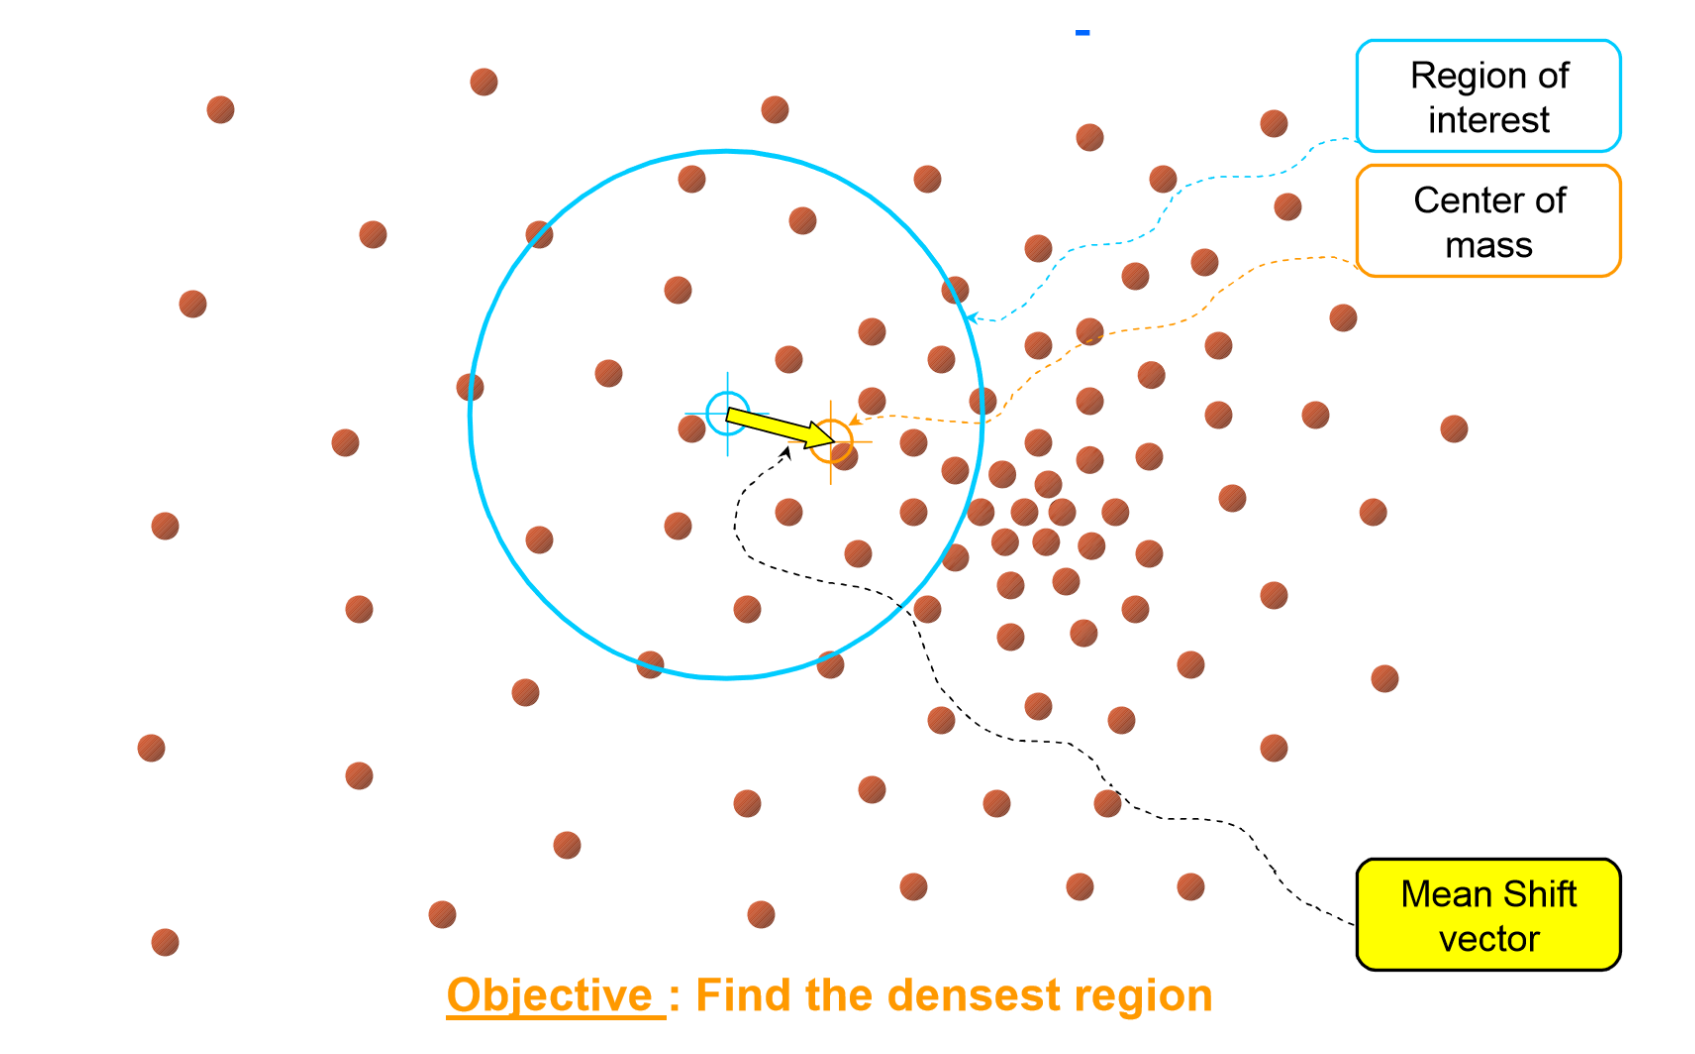
\includegraphics[width=0.8\textwidth]{figures/mean_shift.png}
\caption{Shifting the center of the ROI towards the mean of the center of mass}
\label{fig:mean_shift}
\end{figure} 

The framework of the mean shift tracking is based on choosing some position of the object in the current frame, and searching for it in the neighborhood of it, in the next frame. Maximise the similarity function which can be based on \textbf{Color likelihood (best for single color objects) or represent color distribution with histograms and find the most similar histogram.} 
\begin{figure}[H]
\centering
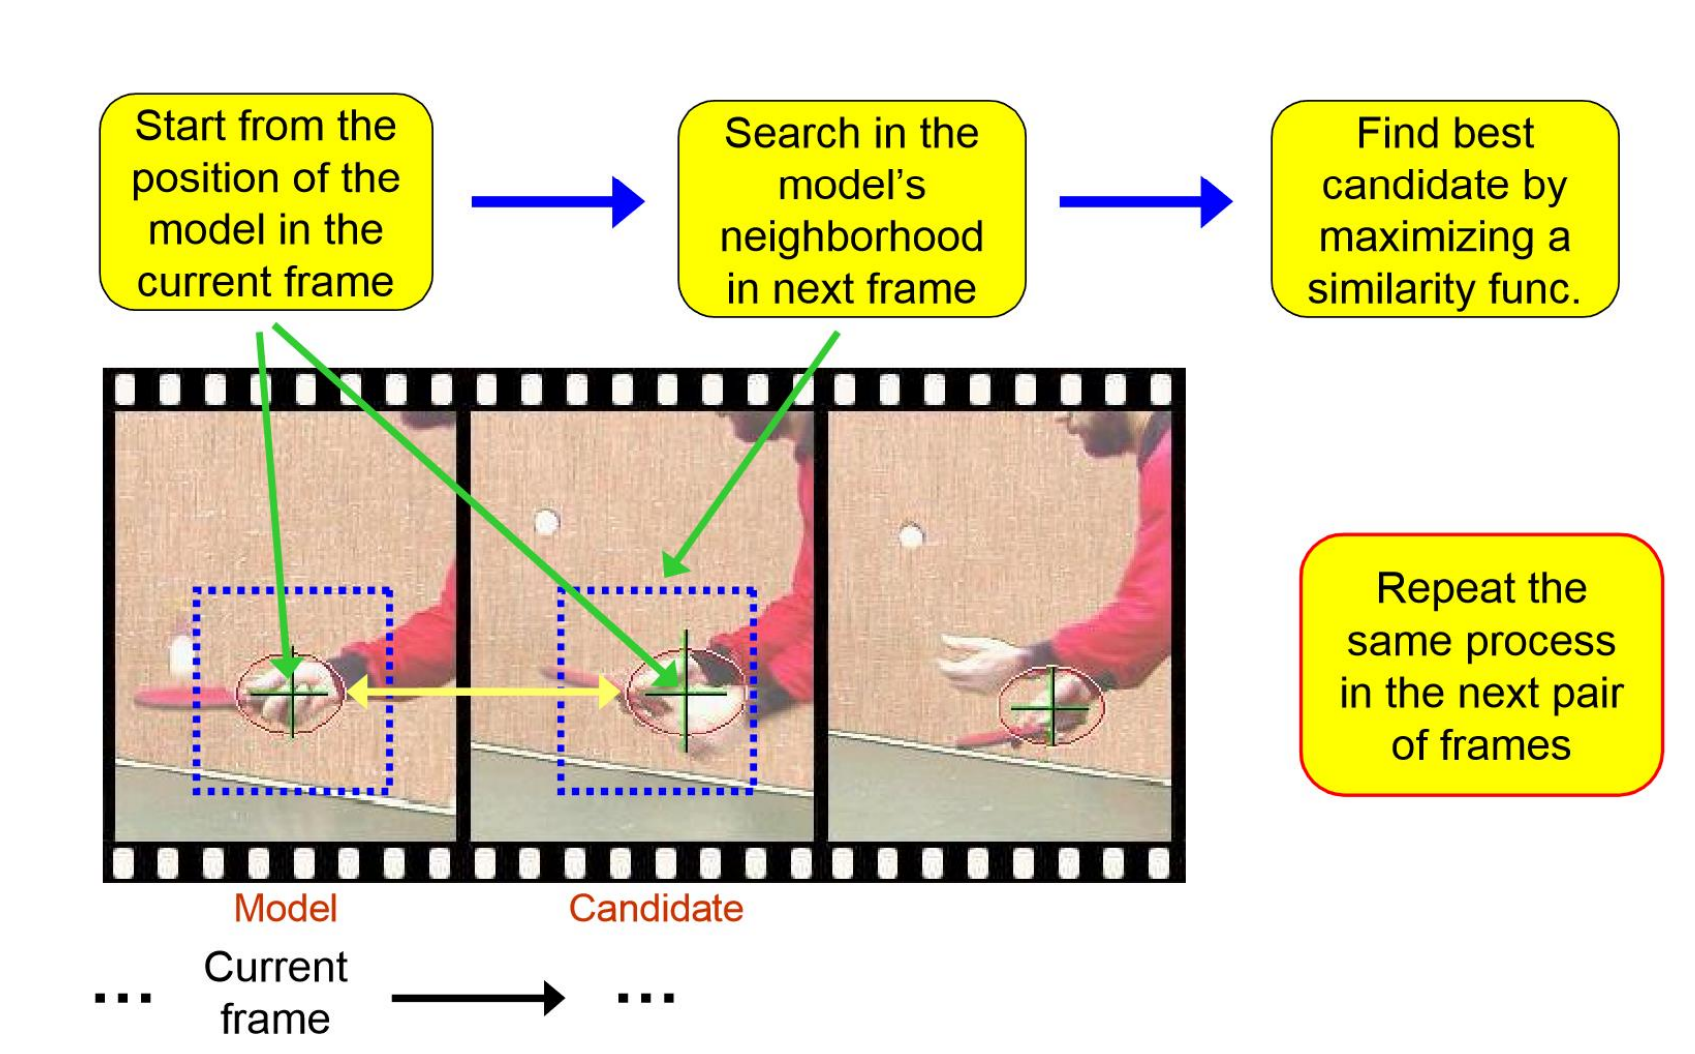
\includegraphics[width=0.8\textwidth]{figures/mean_shift_framework.png}
\caption{Framework of mean shift}
\label{fig:mean_shift_framework}
\end{figure} 

The 1'st method:
\begin{itemize}
	\item Requires good segmentation
	\item Or we compute a likelihood of pixels (what is the probability of this pixel being in the object we are tracking.)
\end{itemize}

The 2'nd method

\begin{figure}[H]
\centering
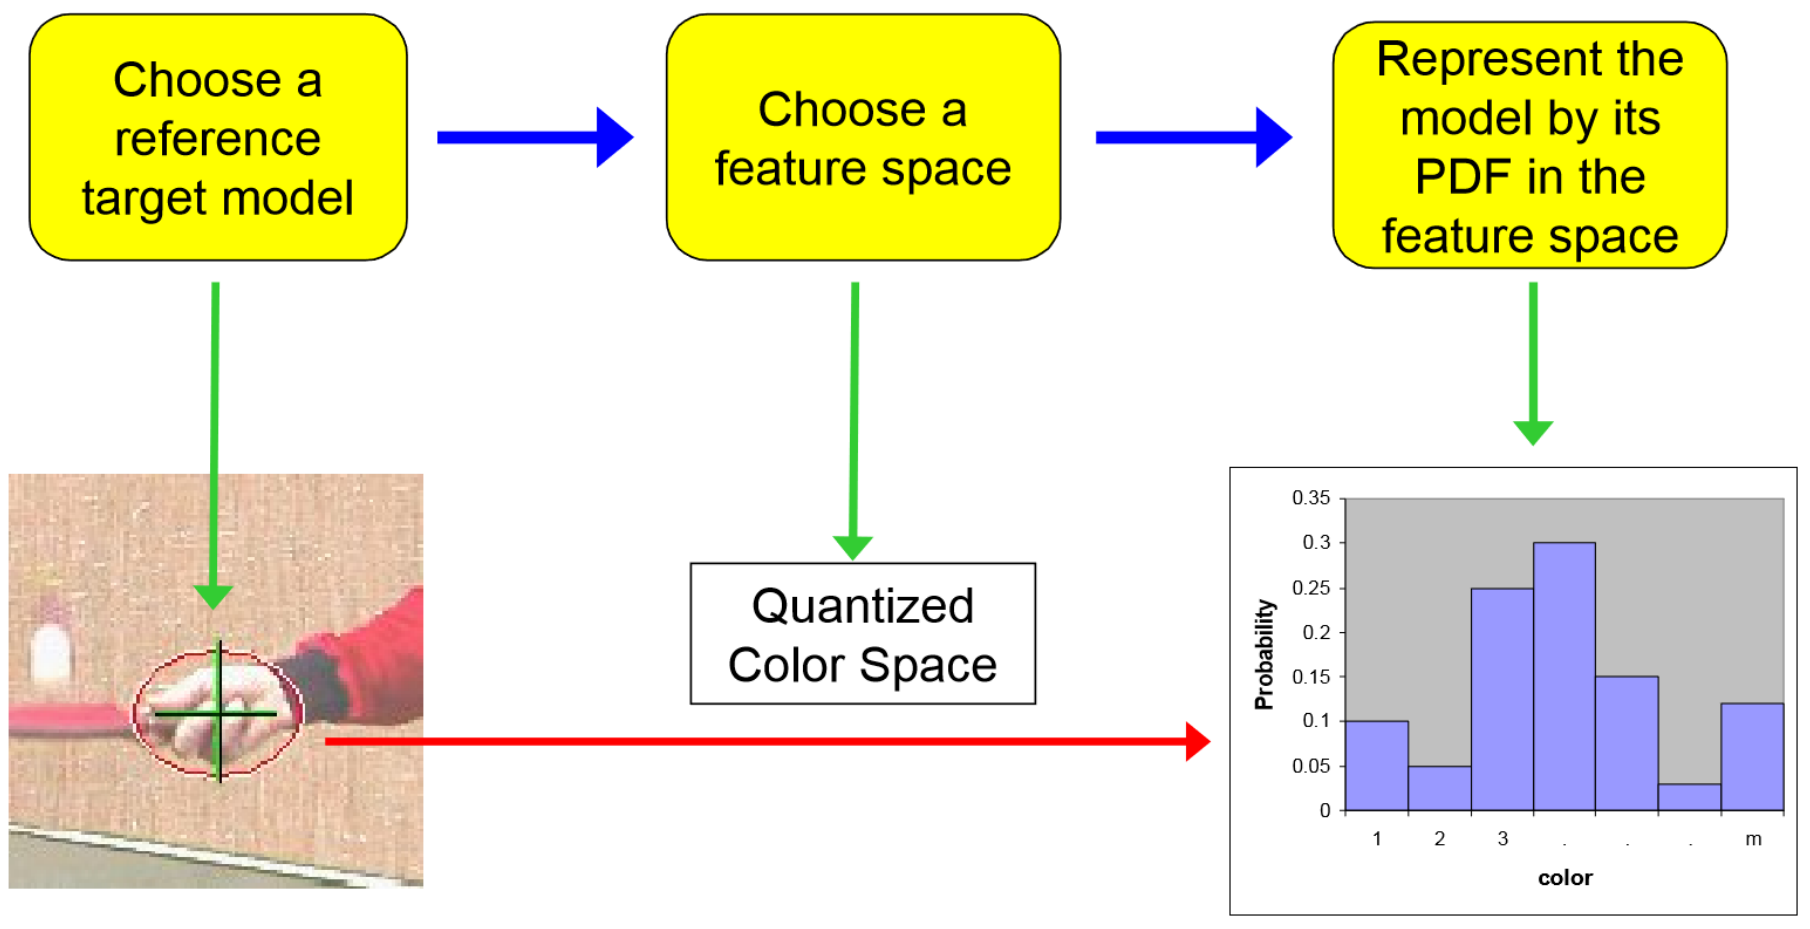
\includegraphics[width=0.8\textwidth]{figures/mean_shift_histogram_likelihood.png}
\caption{Choosing the featurespace and representing the likelihood of the model being the best match based as a PDF.}
\label{fig:histogram_likelihood}
\end{figure} 

% ----------------------------------------------------------------------------------------------------------------------
\newpage
\subsection{Multi Object tracking}
We can just run several independent trackers but there are some problems that must be adressed:
\textbf{Problems:} 
\begin{itemize}
	\item Similar / identical objects
	\item Splits
	\item Merge/ intersections
	\item Occlusions
	\item Noise
\end{itemize}

\begin{figure}[H]
\centering
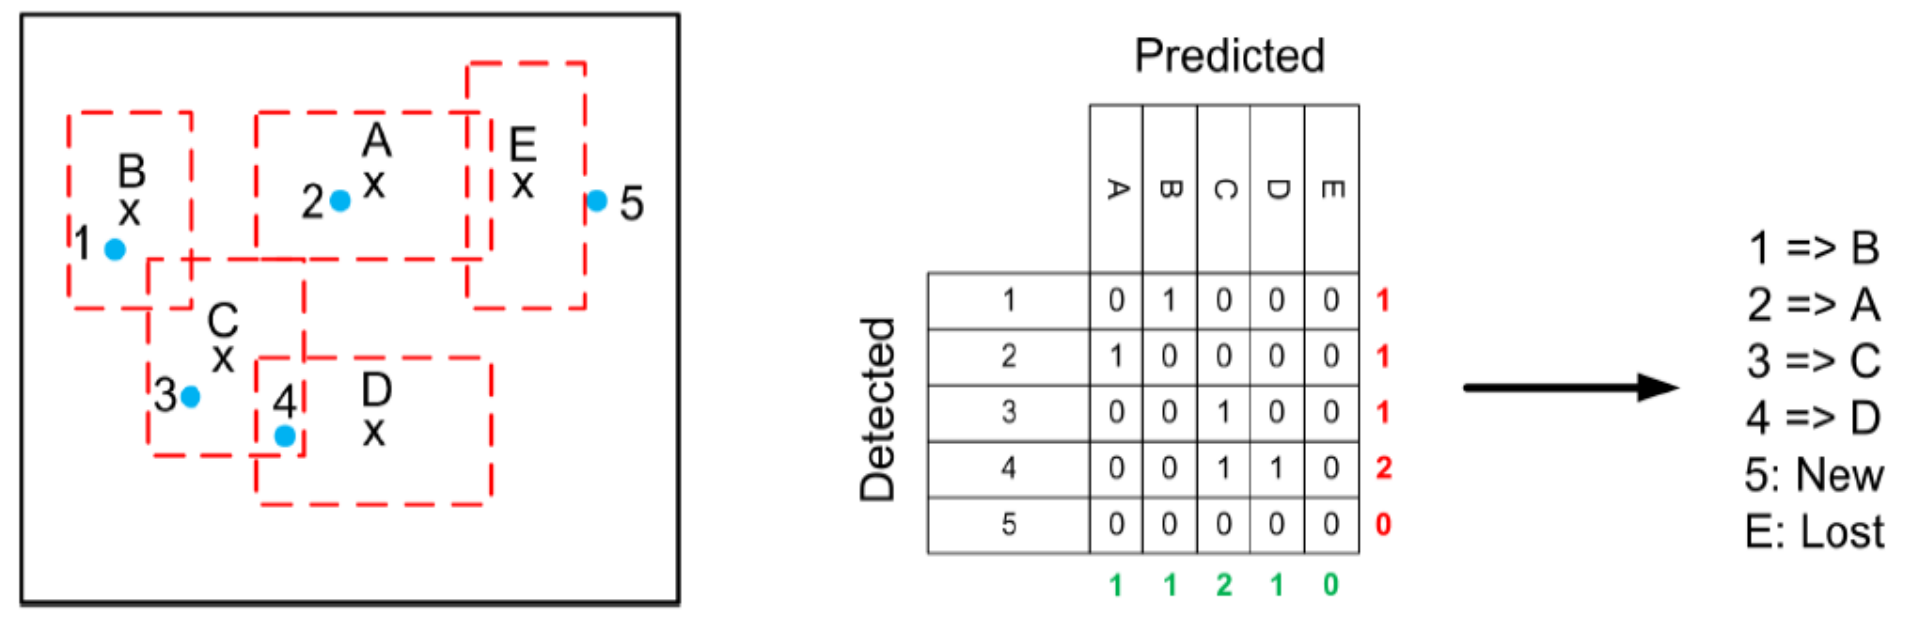
\includegraphics[width=0.9\textwidth]{figures/MOT_example.png}
\caption{Multi Object Tracking example illlustrating issues. }
\label{fig:MOT_example}
\end{figure} 

\begin{figure}[H]
\centering
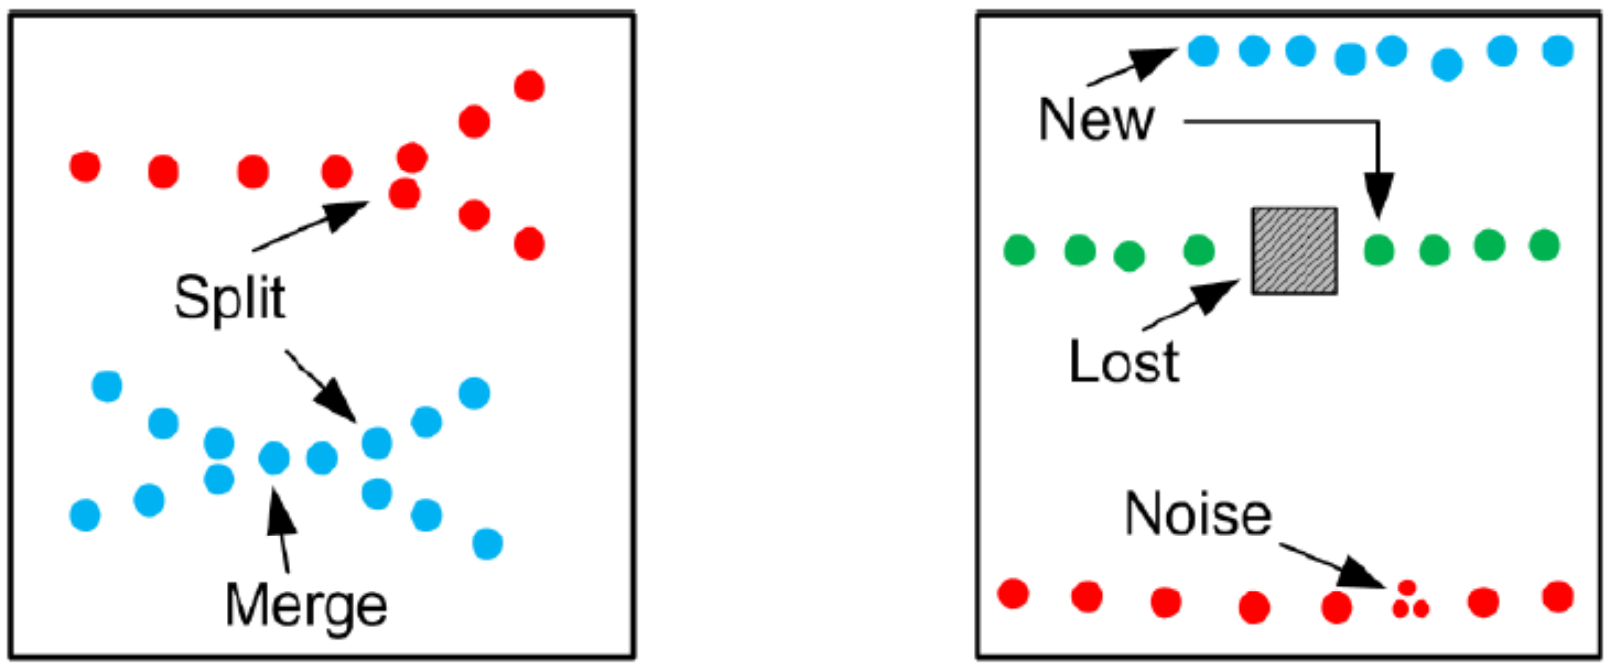
\includegraphics[width=0.9\textwidth]{figures/MOT_issues.png}
\caption{Multi Object Tracking issues.}
\label{fig:MOT_issues}
\end{figure} 

The problem is \textbf{Data association} 
\subsubsection{Hungarian algorithm}
Optimal assignment based on a given cost matrix.

\begin{figure}[H]
\centering
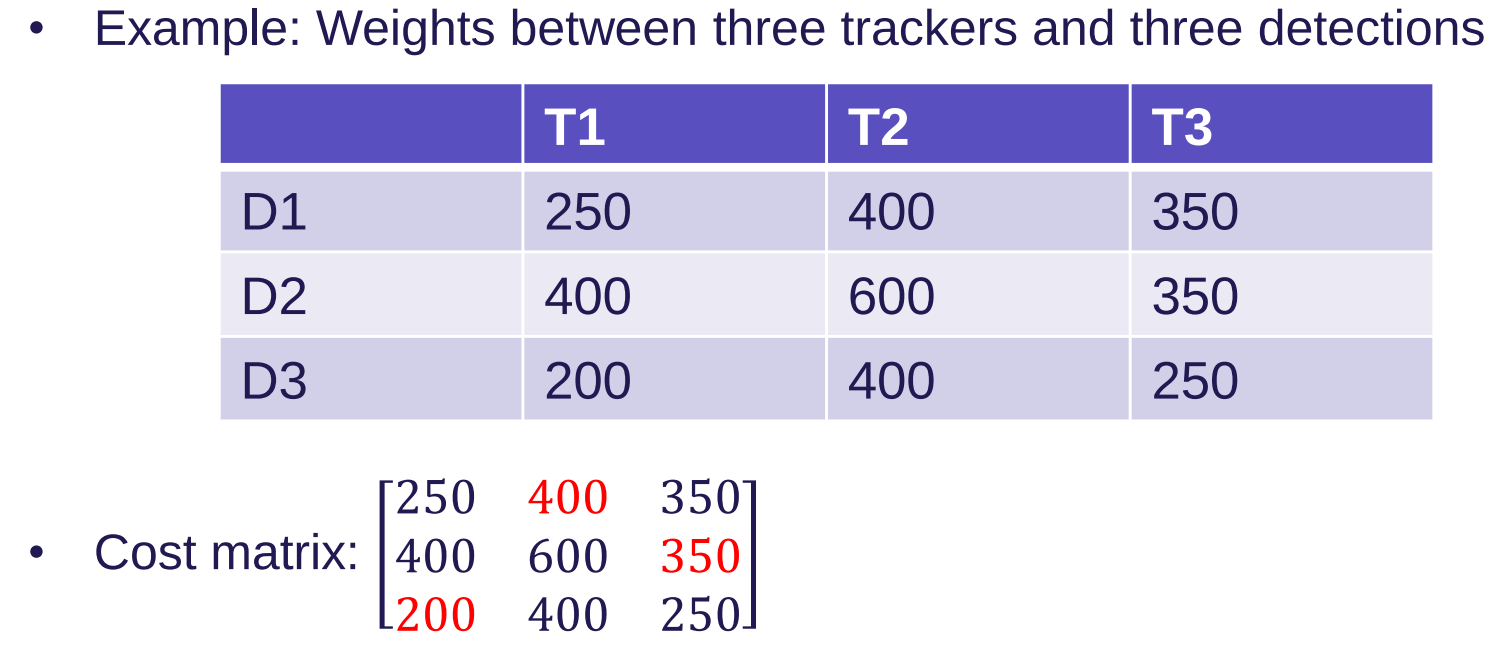
\includegraphics[width=0.7\textwidth]{figures/Hungarian_algorithm.png}
\caption{Hungarian algorithm cost matrix}
\label{fig:hungarian_cost_matrix}
\end{figure} 


% ----------------------------------------------------------------------------------------------------------------------
\newpage
\subsection{Depth sensing}
\textbf{Goal} $ \rightarrow $ recover 3D coordinates from 2D images.

In 2D images, size and distance is unknown.
\begin{figure}[H]
\centering
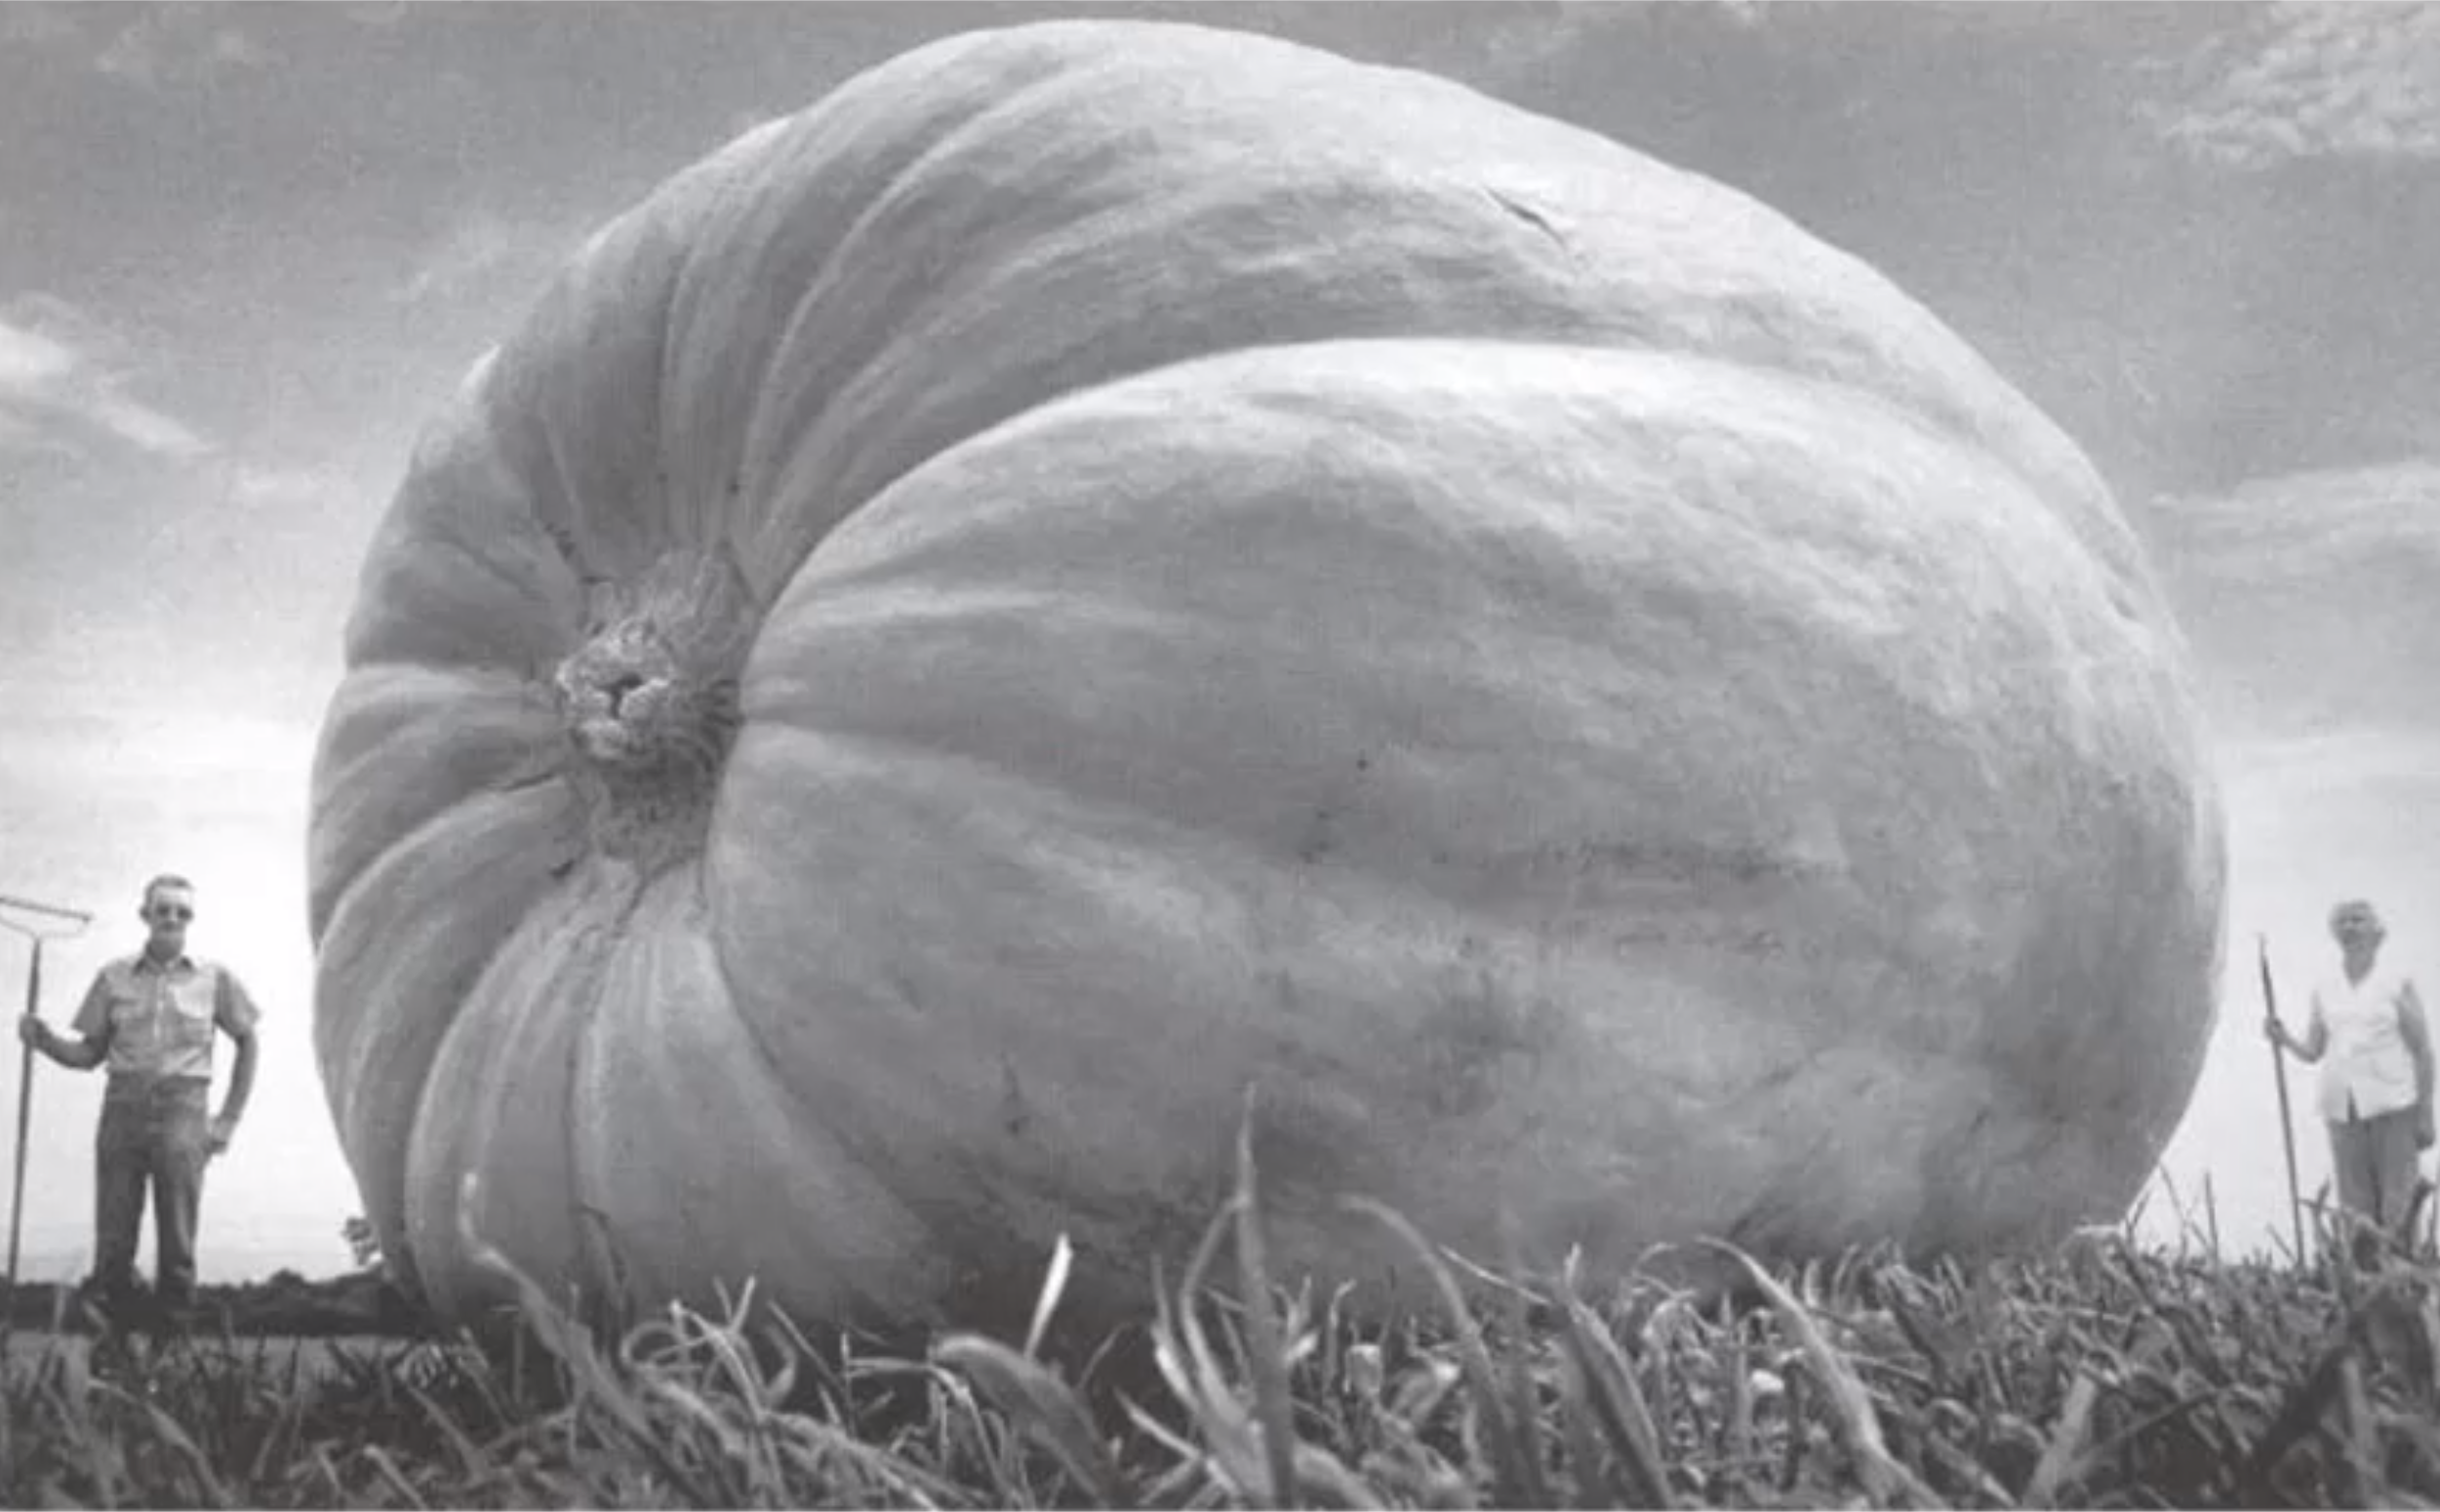
\includegraphics[width=0.9\textwidth]{figures/Depth_illusion.png}
\caption{Depth illusion}
\label{fig:depth_illusion}
\end{figure} 


Different technologies exist in distance measurement. We are working with \textbf{reflective} (transmissive would be the object them selfs transmitting data that can be measured. ) Active optical distance measurement meanst that the camera itself emits some kind of radiation. Passive is when the ambient light is used and measured. 
\begin{figure}[H]
\centering
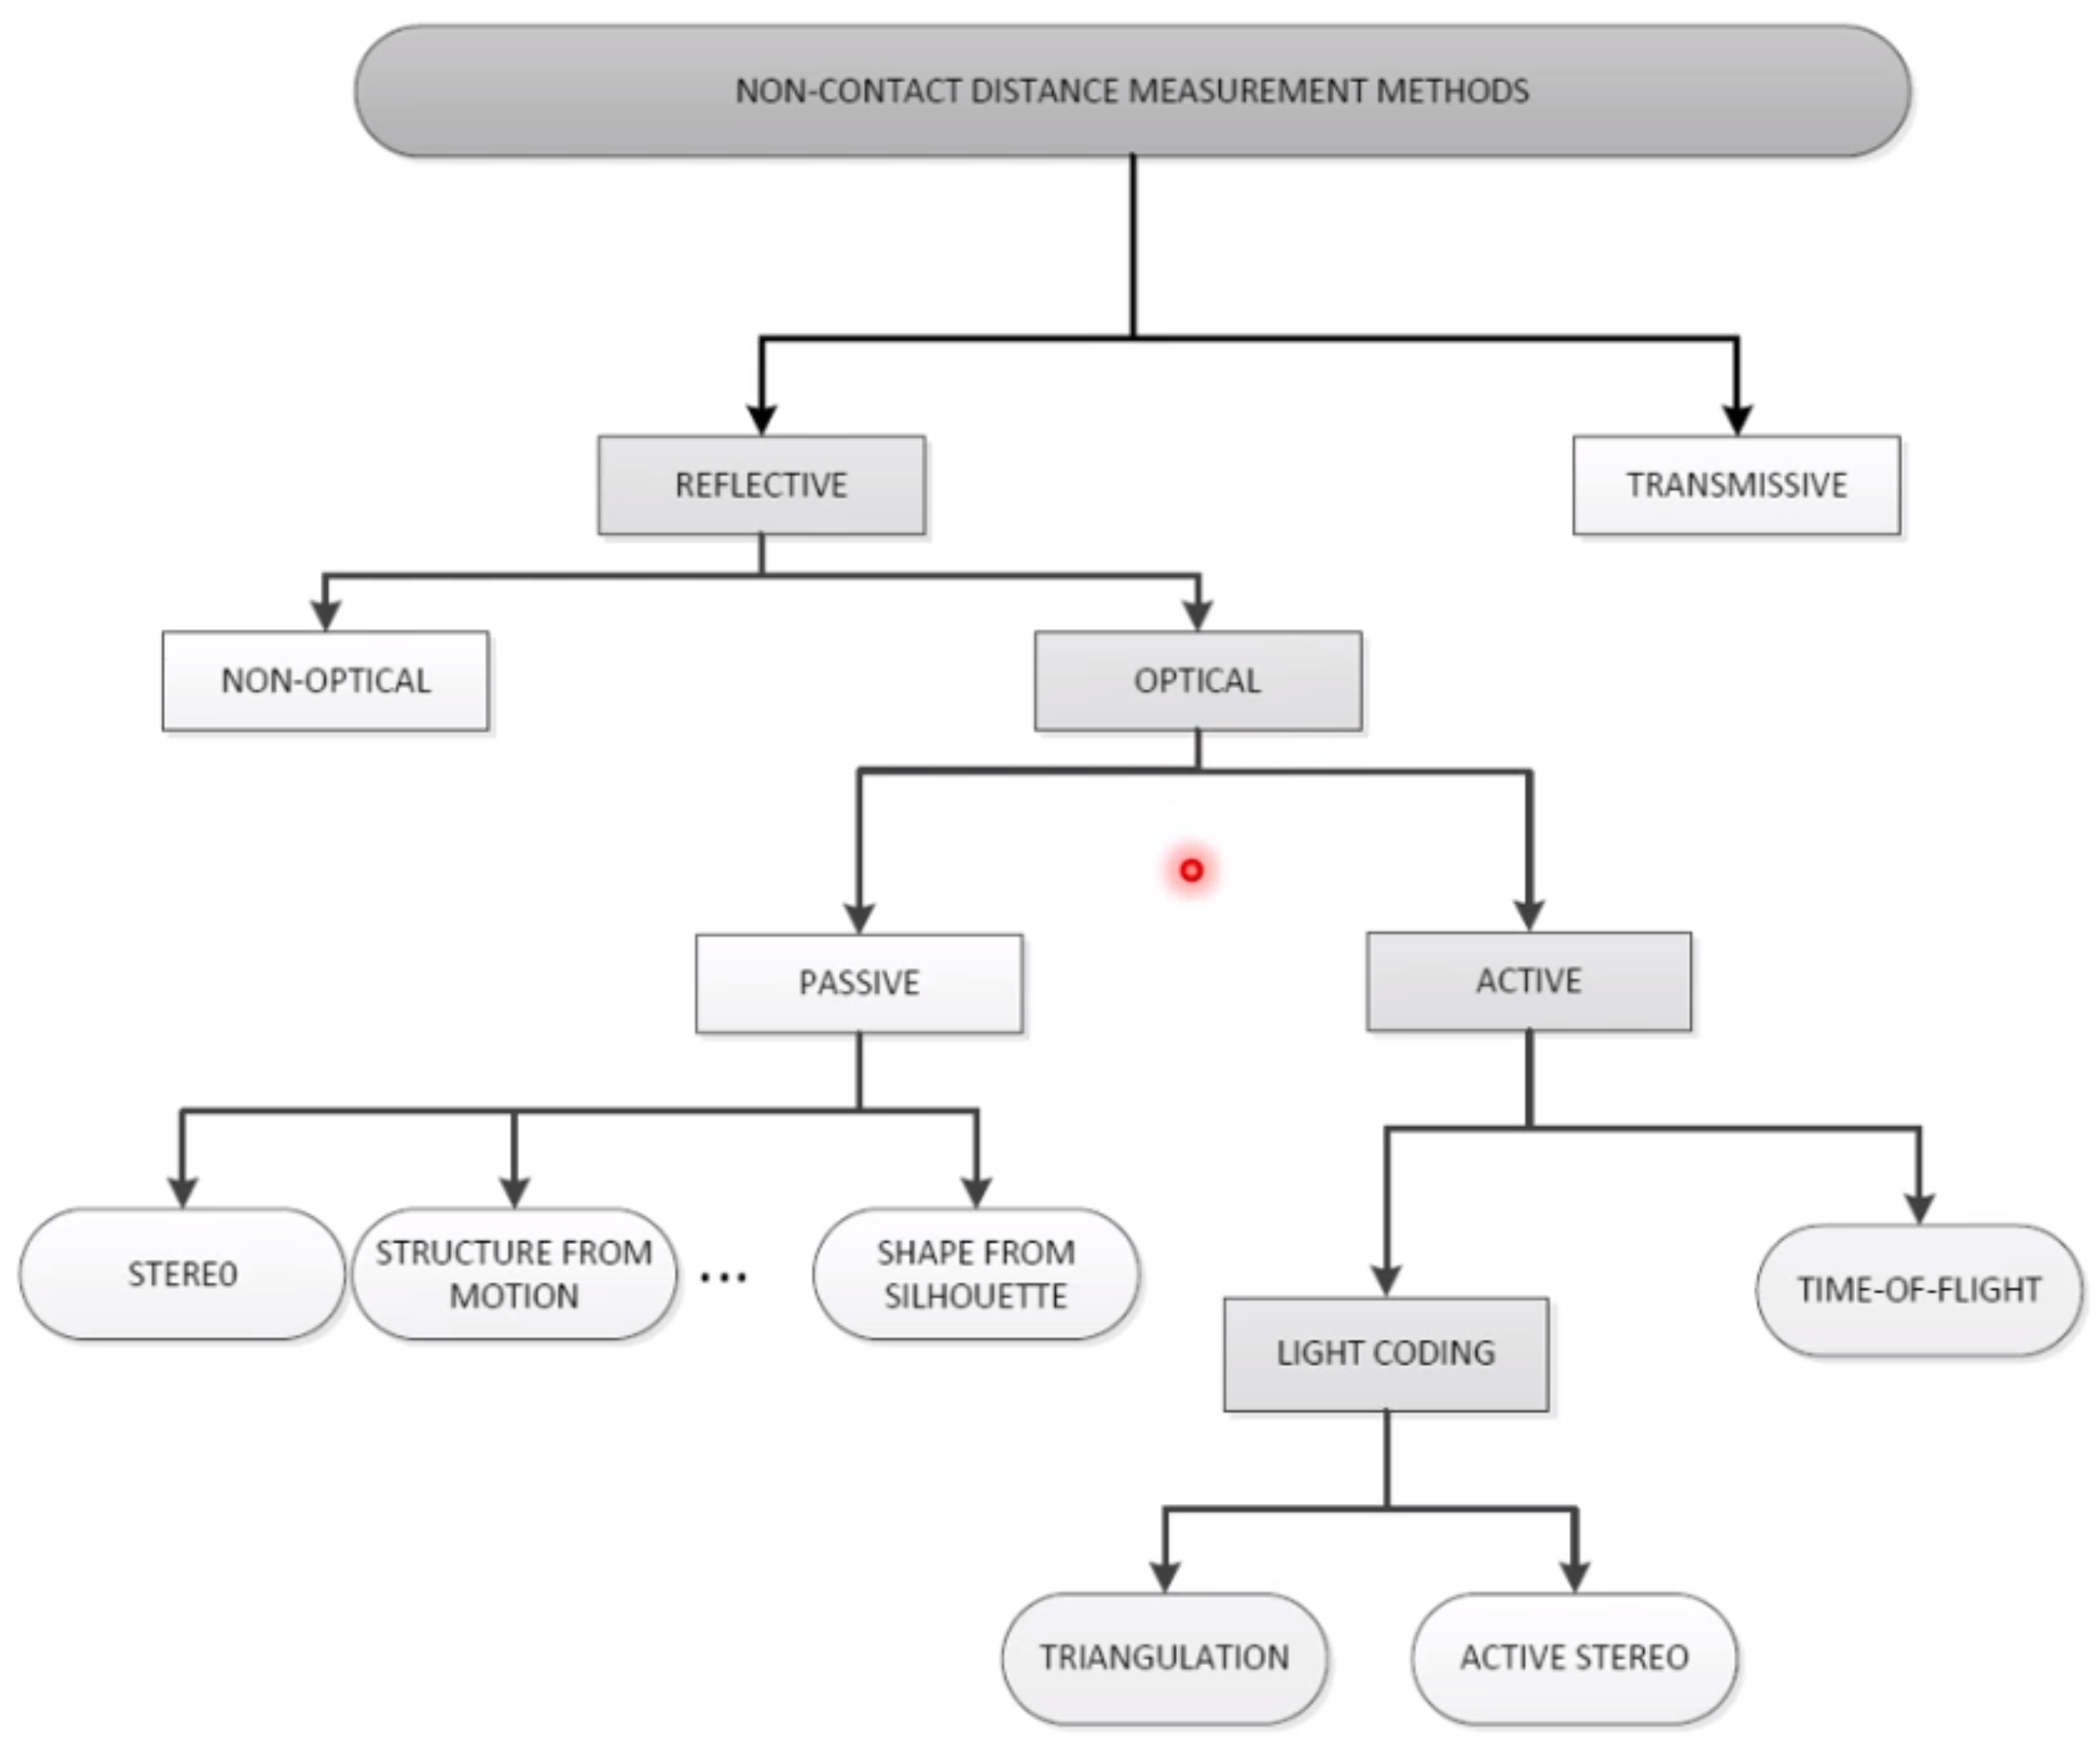
\includegraphics[width=0.9\textwidth]{figures/Types_of_distance_measurements.png}
\caption{Types of distance measurements}
\label{fig:types_of_distance_measurements}
\end{figure} 


\subsubsection{Two view geometry}
\textbf{Aquire image pair} 
\begin{enumerate}
	\item Stero rig (two cameras)
	\item Move one camera and take two fotos.
\end{enumerate}
\vspace{5pt}

A keypoint can be triangulated but it takes two steps:
\begin{enumerate}
	\item Find the keypoint from the 1'st image in the 2'nd image. \textbf{Search problem} 
	\item Estimate the 3D point by triangulation. \textbf{Estimation problem} 
\end{enumerate}

We can reduce the search problem from 2D to 1D using \textbf{Epipolar constraints} 
\begin{figure}[H]
\centering
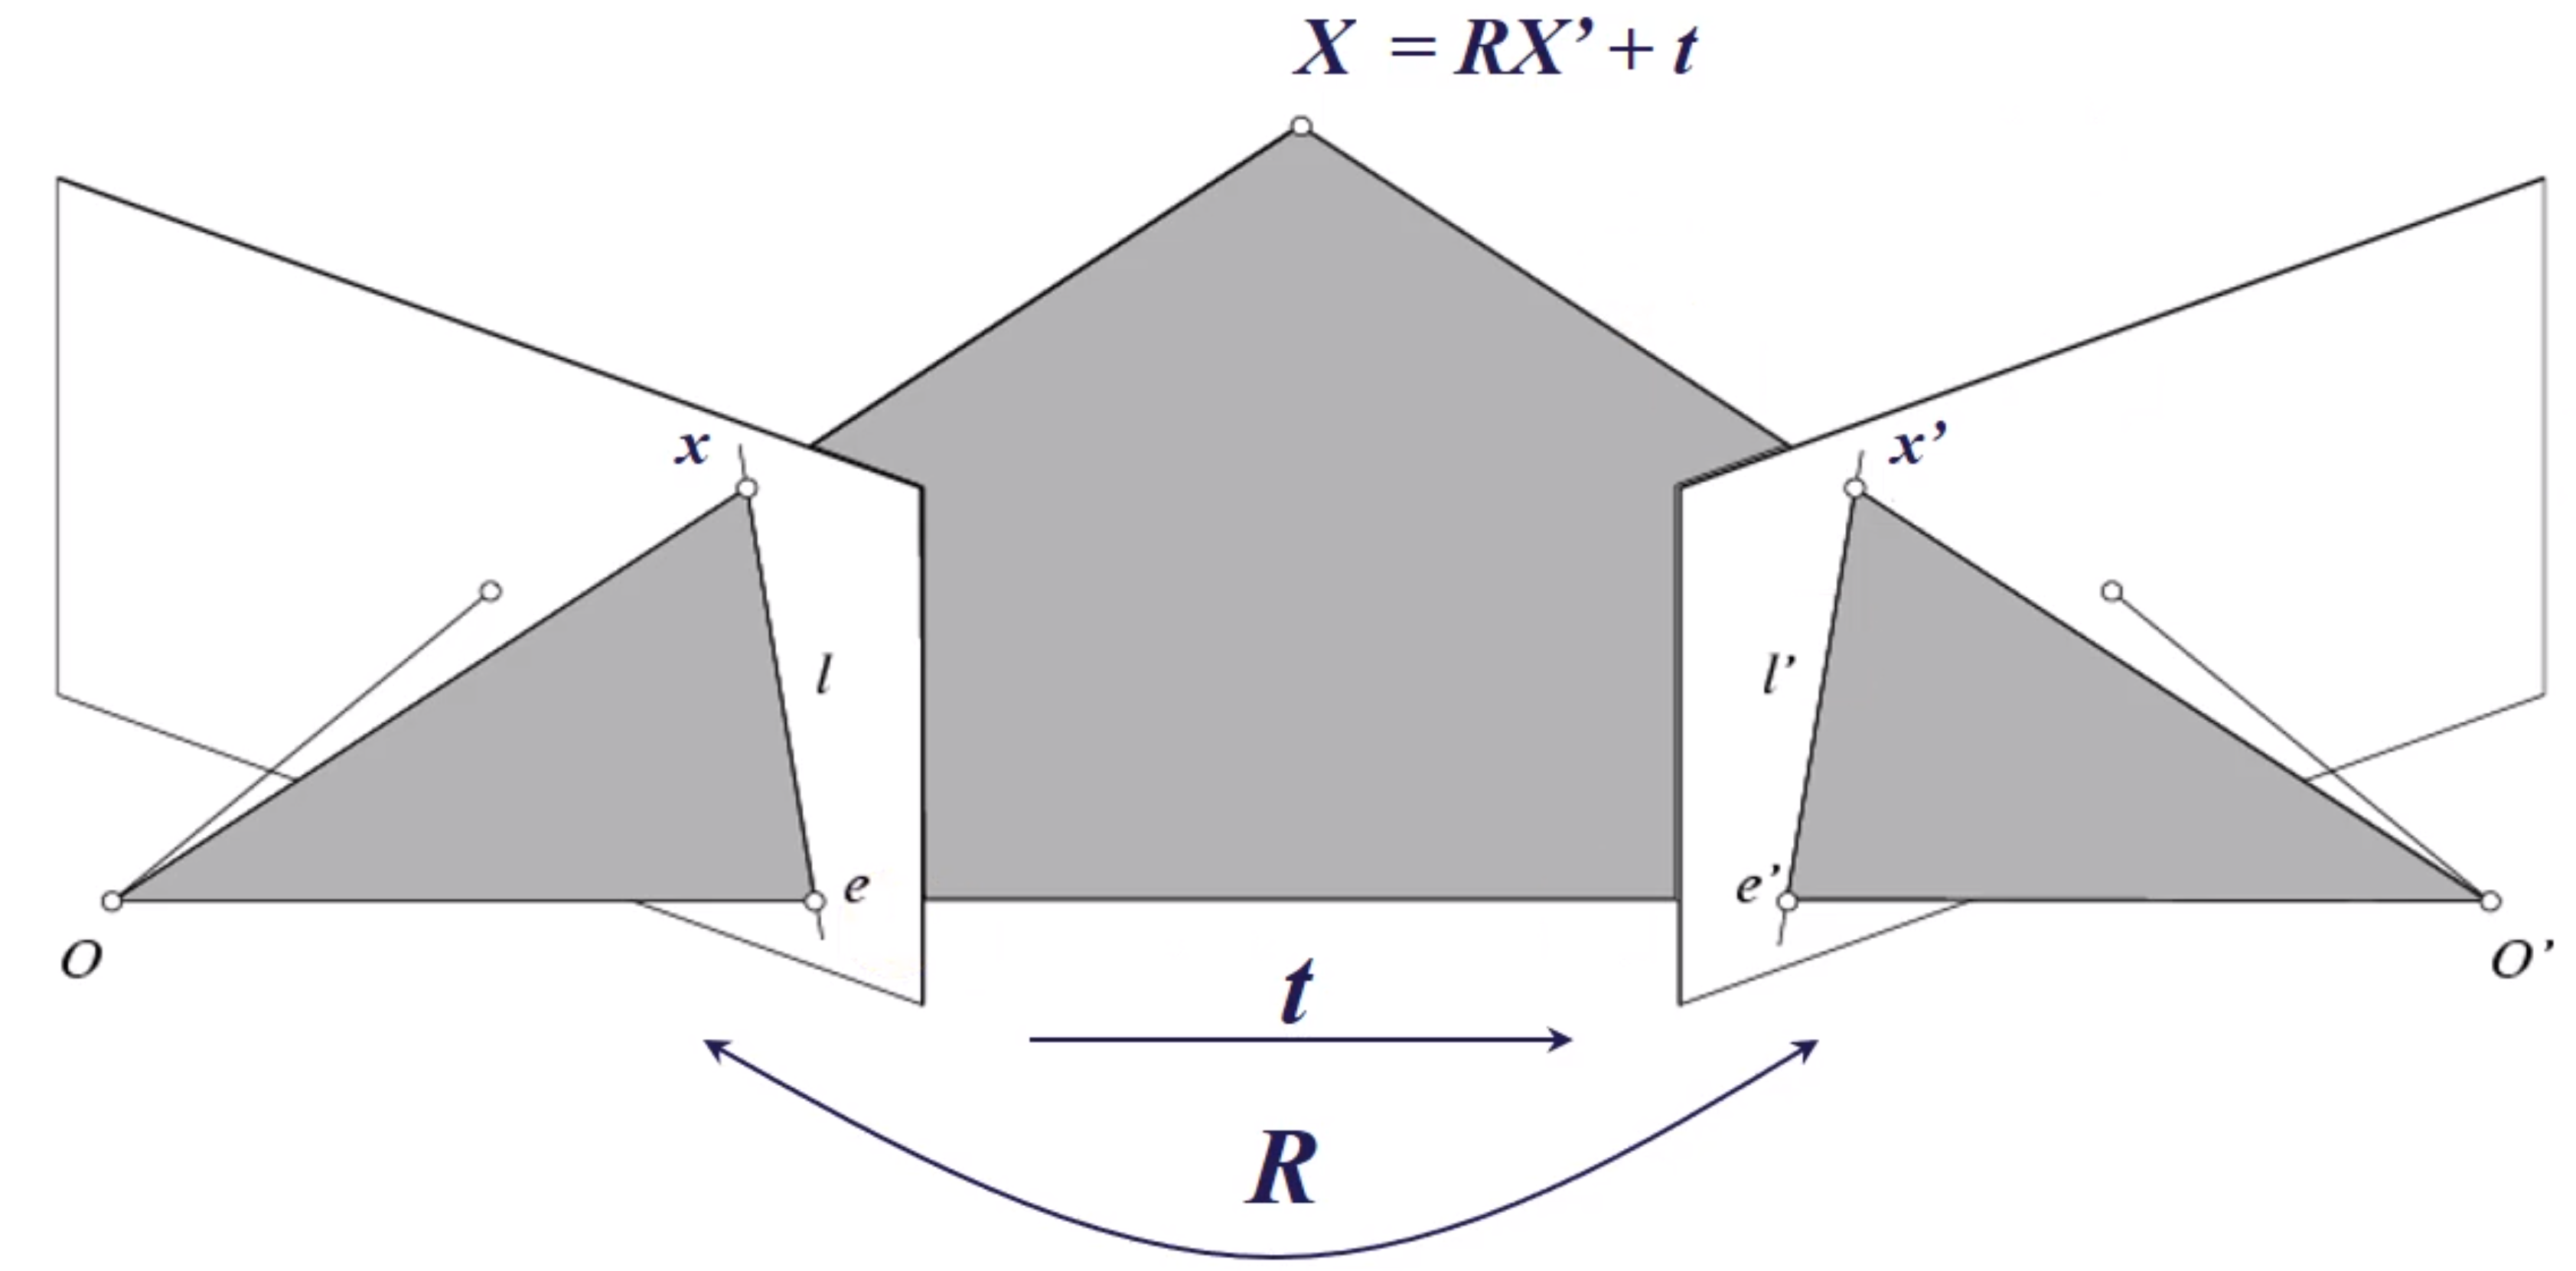
\includegraphics[width=0.9\textwidth]{figures/Epipolar_geomtry.png }
\caption{Epipolar geometry}
\label{fig:Epipolar_geomtry}
\end{figure} 

\begin{itemize}
	\item \textbf{Baseline:} line between the two cameras
	\item \textbf{Epipolar plane:} plane between the two point camera's. Contains the baseline. Rotates around the baseline
	\item \textbf{Epipoles:} intersections of baseline with image planes. (may be outside of the frame)
	\item \textbf{Epipolar Lines:} Intersection between the epipolar plane and the epipolar image planes. 
\end{itemize}

Epipoles are at infinity when the two image planes are parallel. But when we have \textbf{Converging } cameras, then the epipoles exist. 

\textbf{Assumes} we know extrinsic and intrinsic parameters (Camera is calibrated). 

We compute the \textbf{Essential matrix} 
\begin{equation}
	E = [t_{\times}]R
\end{equation}
\begin{equation}
	[t_{\times}] = \begin{bmatrix}
	0 & -t_3 & t_2\\
	t_3 & 0 & -t_1\\
	-t_2 & t_1 & 0
	\end{bmatrix}
\end{equation}
Where $ [t_{\times}] $ is a decomposition of the translation vector.
	 

Using the essential matrix we get an equation for the epipolar line for point $ x' $ in the other image.
\begin{equation}
l = E x'
\end{equation}

We use the \textbf{Fundamental} matrix $ F $ if the camera is \textbf{uncalibrated} 

\subsubsection{Depth sensing with two view geometry}
Using a calibrated camera pair (know both extrinsic and intrinsic)

\begin{enumerate}
	\item Calibrate camera (offline)
	\item Aquire image pair (online $ \rightarrow $  )
	\item Rectify images (Align points along the same horizontal scanline.)
	\item Compute horizontal disparity (unit = pixels) \\
	\begin{itemize}
		\item Dense (for every pixel) $ \rightarrow $ scan along the scanline and do e.g. Sum of squared differnces or normalized correlation and find the best match.
		\item Sparse (for keypoints)
	\end{itemize}
	\item Triangulate to optain 3D coordinate. (unit = meters)
\end{enumerate}

Requires parallel camera planes. 
For converging cameras, we can project the image planes onto a common plane. (Stereo image rectification)

\begin{figure}[H]
\centering
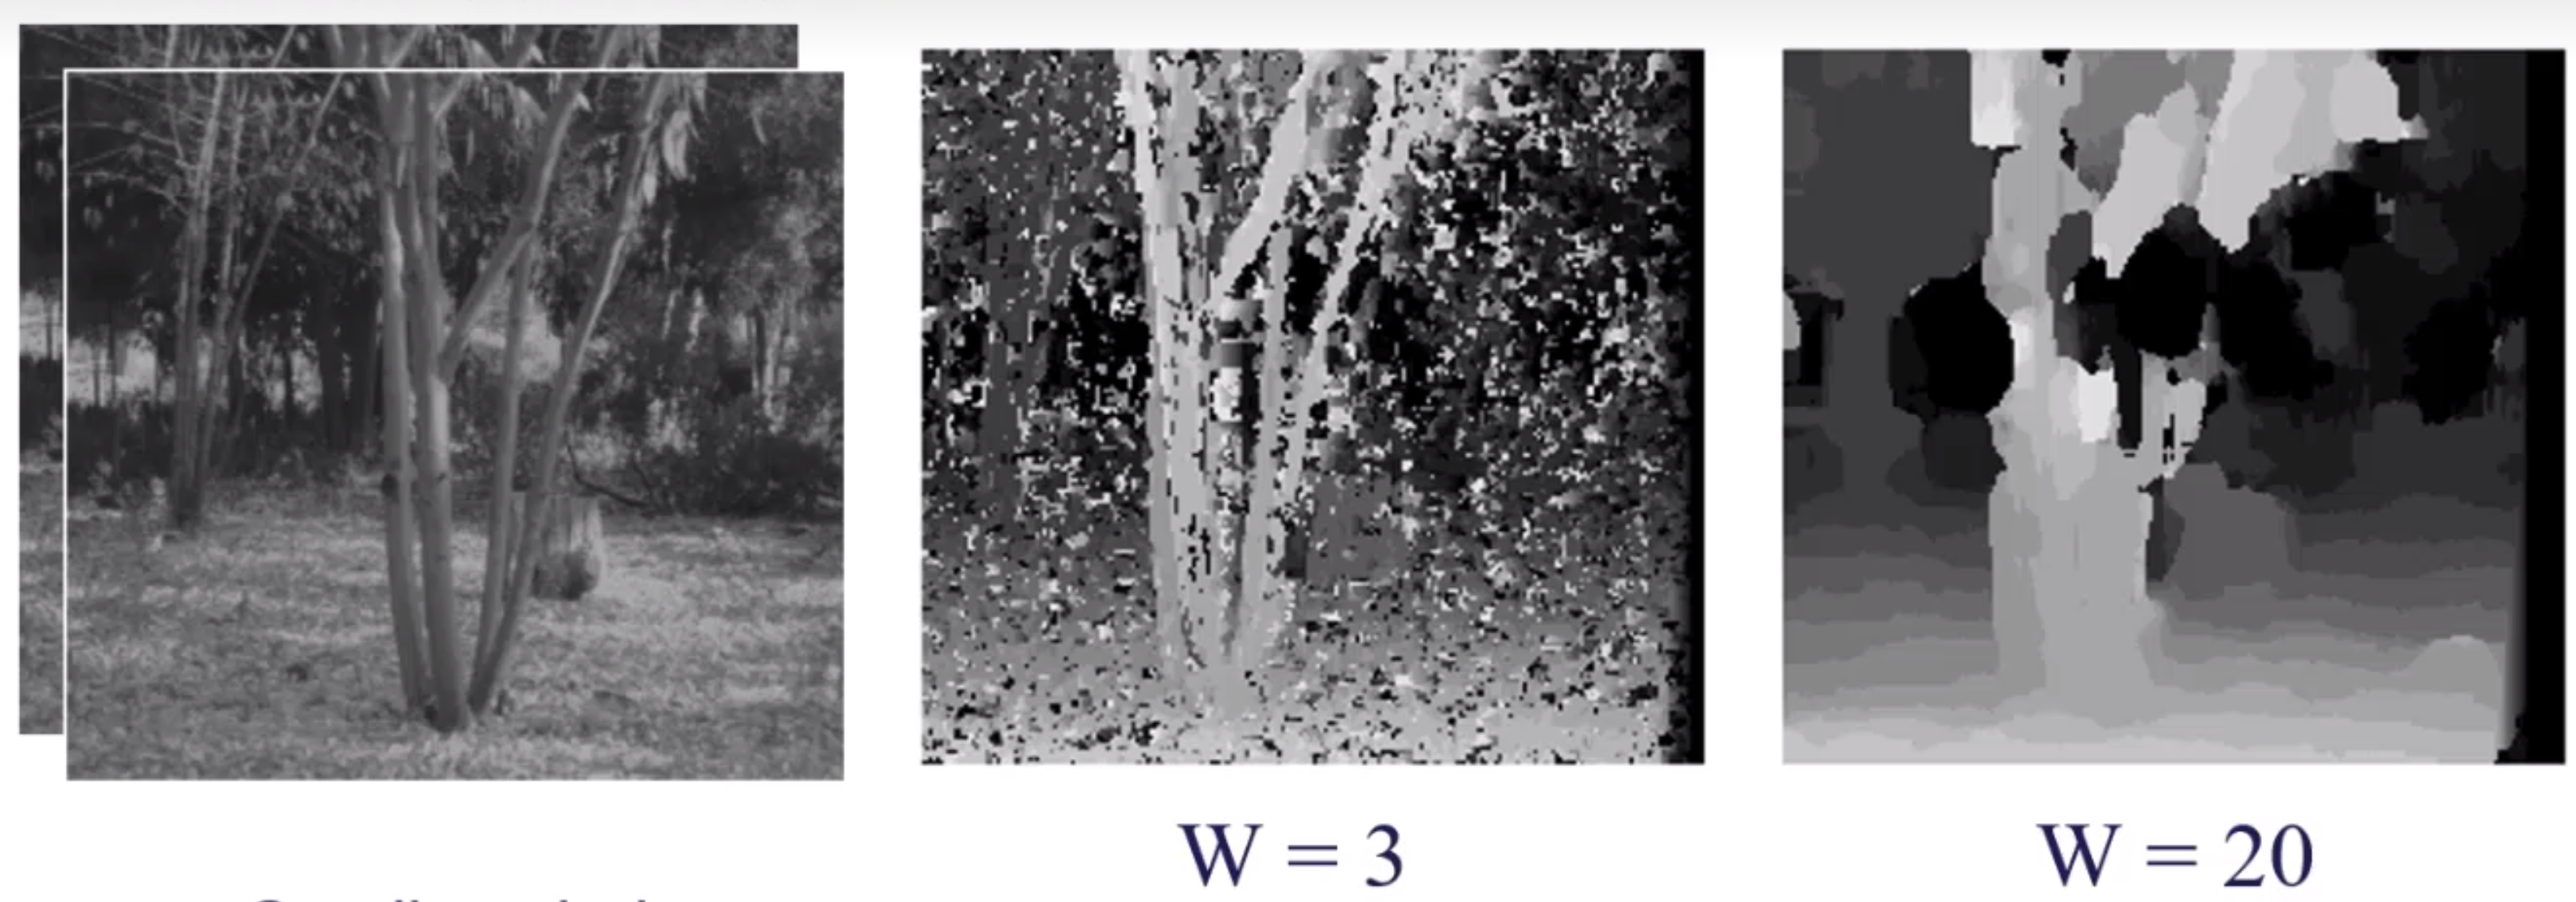
\includegraphics[width=0.99\textwidth]{figures/Window_size_correspondence_noise.png}
\caption{The efffect of window size when doing correspondence in horizontal disparity map}
\label{fig:window_size_correspondence_noise}
\end{figure} 

\begin{itemize}
	\item Large window $ \rightarrow $ less noise and less detail
	\item Small window $ \rightarrow $ more noise and more detail
\end{itemize}

The problems of correspondence search
\textbf{Problems:} 
\begin{itemize}
	\item Occlusions
	\item No texture on surfaces $ \rightarrow $ sacrified uniquness of non-local constraints.
	\item There may be repititions of the same object in the image. (Bars in a fence)
	\item Light may reflect differently in both images. (The images are not similar)
\end{itemize}

\textbf{Depth from disparity} 

\begin{figure}[H]
\centering
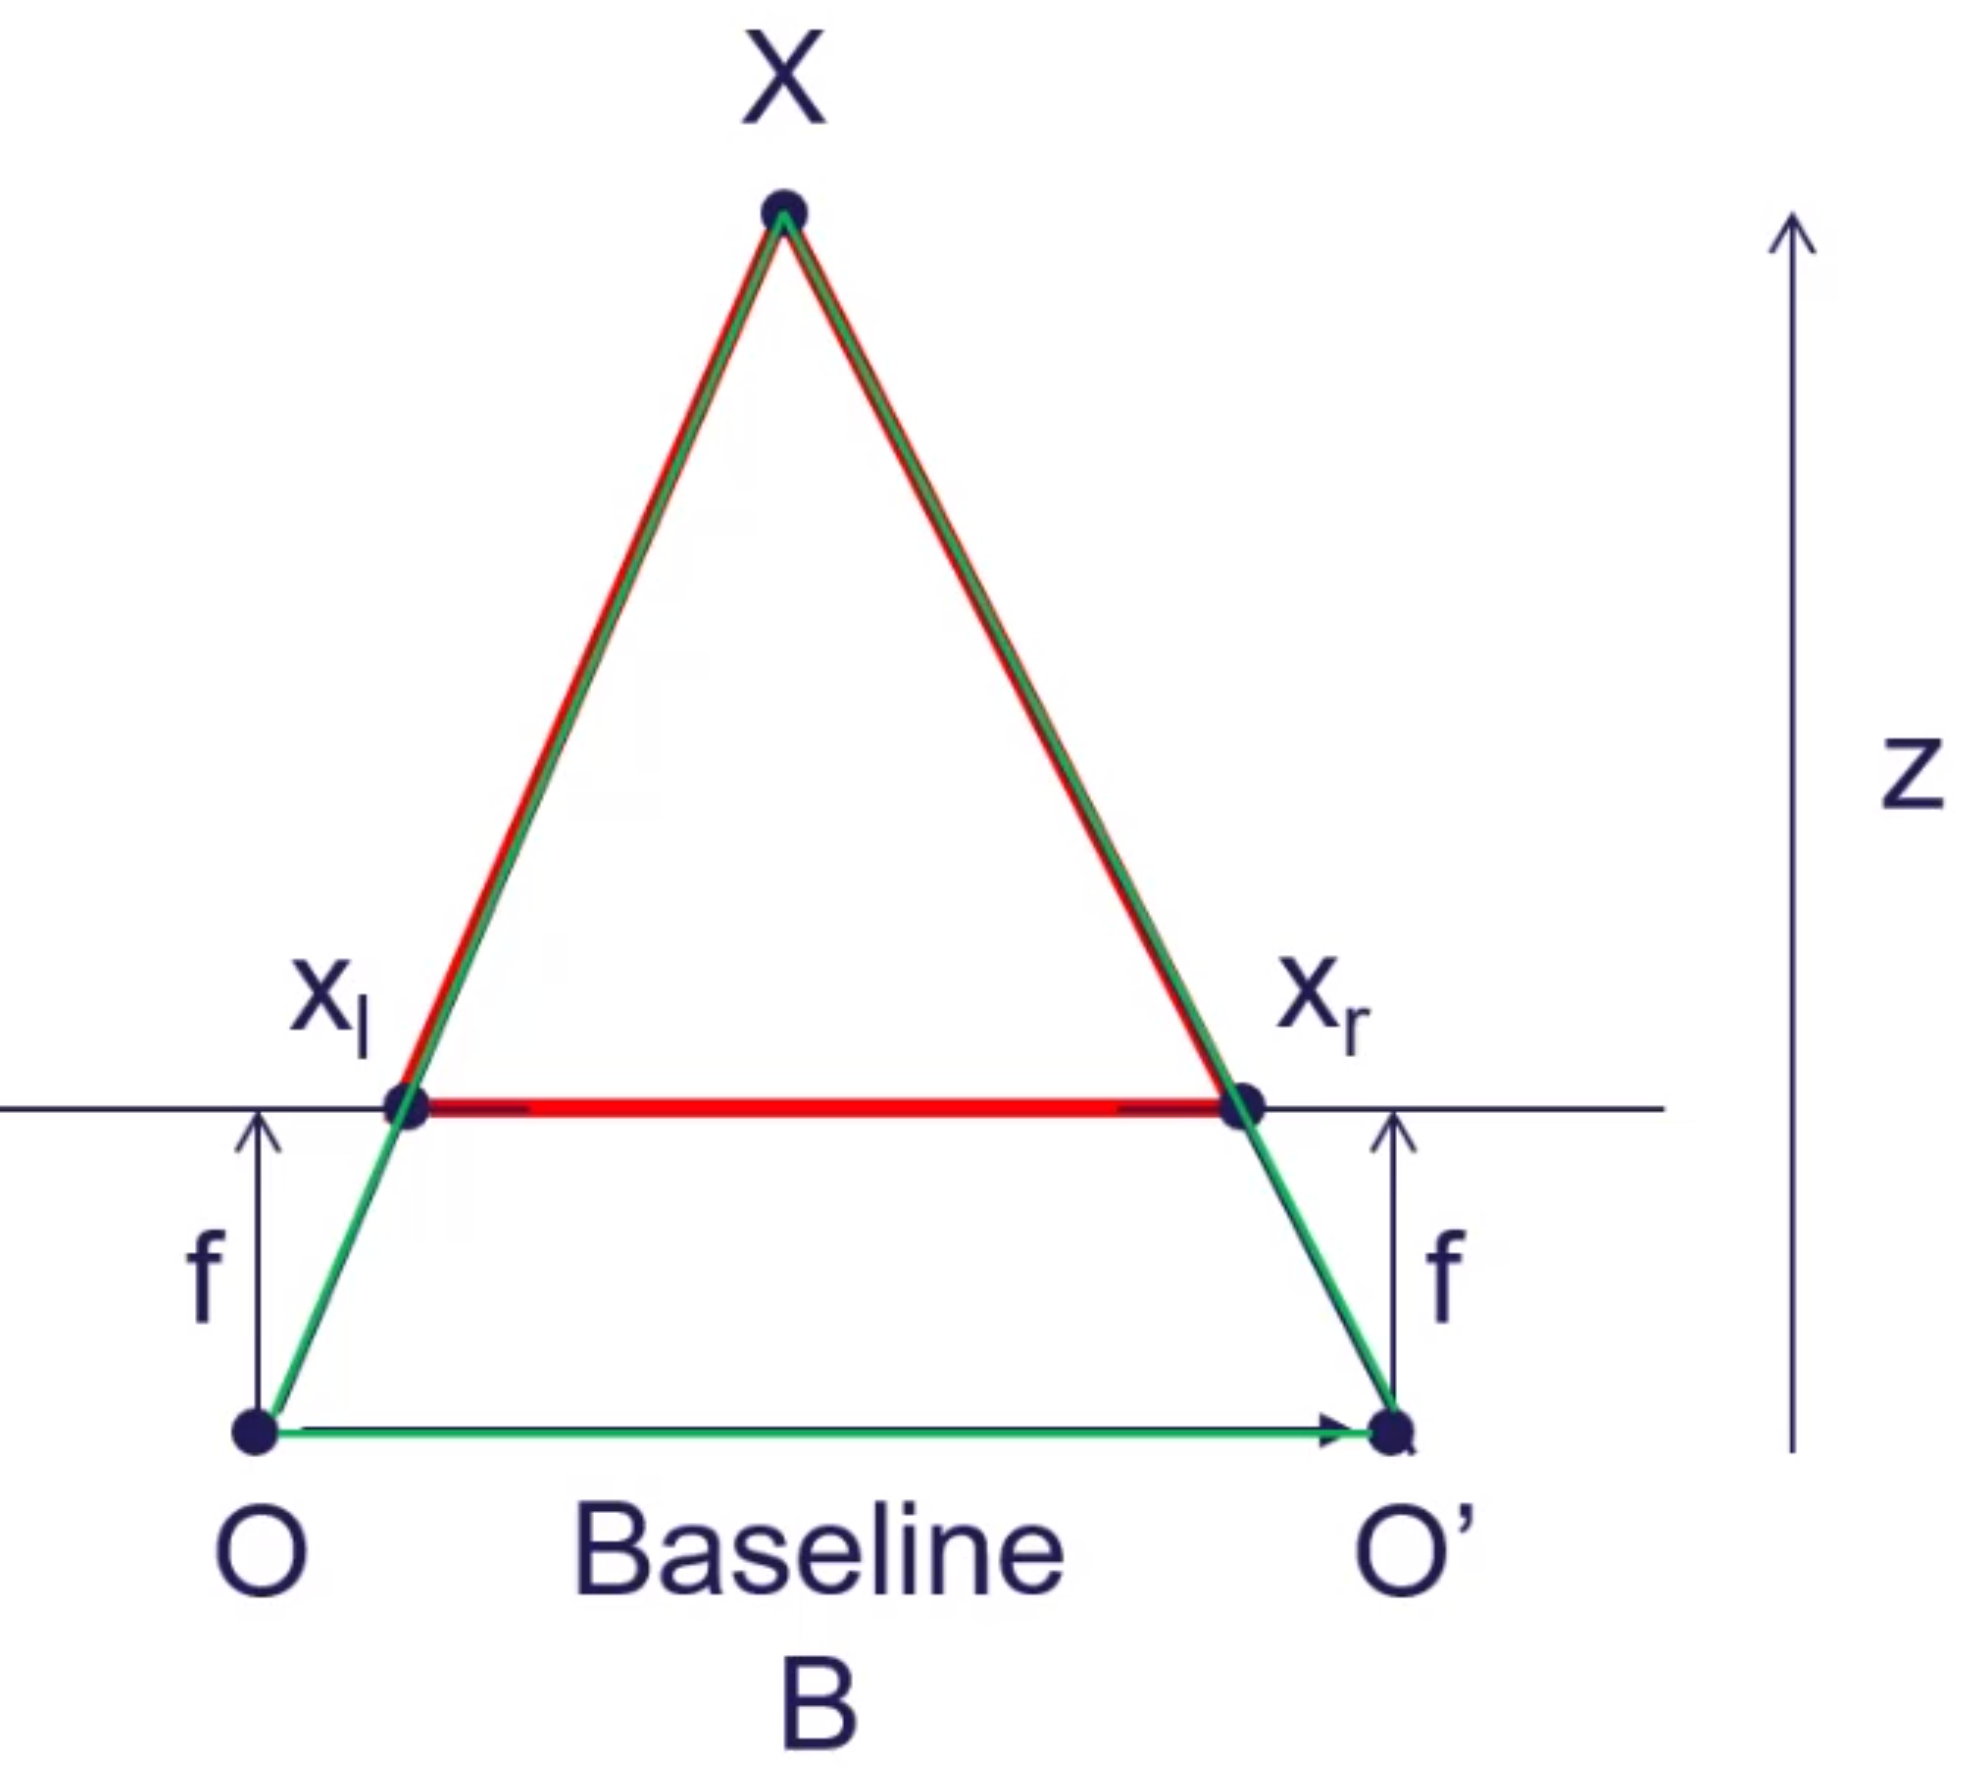
\includegraphics[width=0.6\textwidth]{figures/Depth_from_disparity.png}
\caption{Depth from disparity}
\label{fig:detph_from_disparity}
\end{figure} 

Based on equal triangles, we can compute the ratio, and then get the detph coordinate $ z $
 \begin{equation}
z = \frac{fB}{x_r - x_l} 
\end{equation}

$ x_r - x_l $ is the disparity.\\
It results in discretisisation where the steps gets larger the further it goes, the lower the resolution of the depth estimate.

\subsubsection{Active depth sensors}
\textbf{Structured Light} 
\begin{itemize}
	\item Projects light patterns onto the object
	\item Can estimate depth from \textbf{textureless} objects
\end{itemize}

\textbf{Time of flight} 
\begin{itemize}
	\item Measure the reflection time of a light pulse.
	\item Measure the reflection based on continuously emitted light, and measure  \textbf{phase shift}. 
	\item Both require very high clock speed.
\end{itemize}



% ----------------------------------------------------------------------------------------------------------------------
\newpage
\subsection{Camera calibration, Hand-eye calibration}
\subsubsection{Camera calibration}
In the \textbf{Projective world} parallel lines may meet, and circles may be eliptic (formally known as \textbf{conic}), angles between lines may also change. \\

The mapping from euclidean space to projective space, is done using homogeneous coordinates. 

\begin{itemize}
	\item \textbf{Intrinsic:} estimating internal propoties of the camera that affects the imaging process.
	\item \textbf{Extrinsic:} Estimating the relationship between the world coordinates and the camera coordinates, and object coordinates. 
\end{itemize}
\begin{figure}[H]
\centering
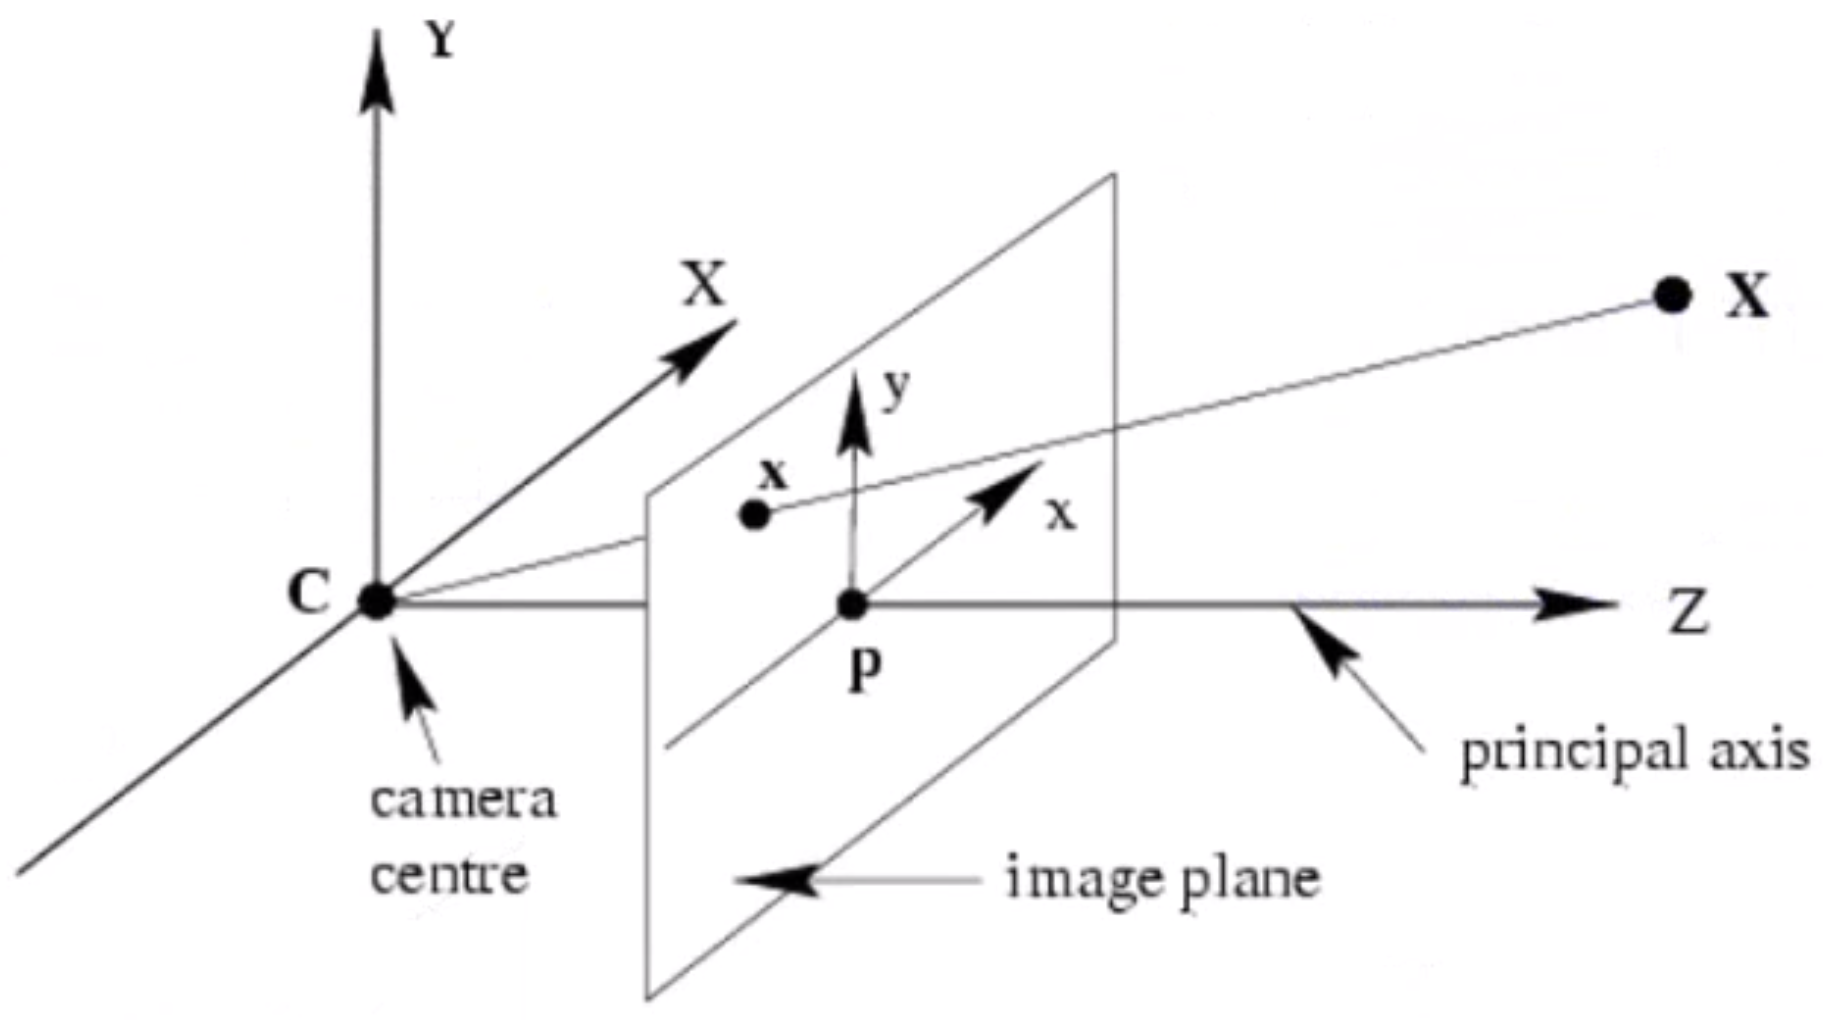
\includegraphics[width=0.5\textwidth]{figures/pinhole_camera_model.png}
\caption{Pinhole camera model}
\label{fig:pinhole_model}
\end{figure} 

For the pinhole camera model we have:
\begin{itemize}
	\item \textbf{Principal axis: } the axis from the camera center perpendicular to the image plane.
	\item \textbf{Normalized (camera) coordinate system: } is the camera center at the origin. Principal axis as the $ z $-axis.
\end{itemize}

We want to estimate the projection matrix $ P \in \mathbb{R}^{4 \times 3}  $ s.t. 
\begin{equation}
x = PX
\end{equation}
where $ x \in \mathbb{R}^{3 \times 1}  $ is the image point and $ X \in \mathbb{R}^{4 \times 1} $ is the scene point. So these are in homogeneous coordinates.

\subsubsection*{Homogeneous coordinates}
We introduce a new variable $ w $ so 3D coordinates in euclidean space is 4D in homogeneous coordinates and 2D $ \rightarrow $ 3D

\begin{equation}
x = \begin{bmatrix}
x \\
y
\end{bmatrix} \leftrightarrow \begin{bmatrix}
u \\
v \\
w
\end{bmatrix} = k \begin{bmatrix}
u \\
v \\
w
\end{bmatrix} 
\end{equation}

We still only have 2 degrees of freedom, so we can extract euclidean points 
\begin{equation}
	x = \frac{u}{w} \hspace{15pt} y = \frac{v}{w} 
\end{equation}


\begin{figure}[H]
\centering
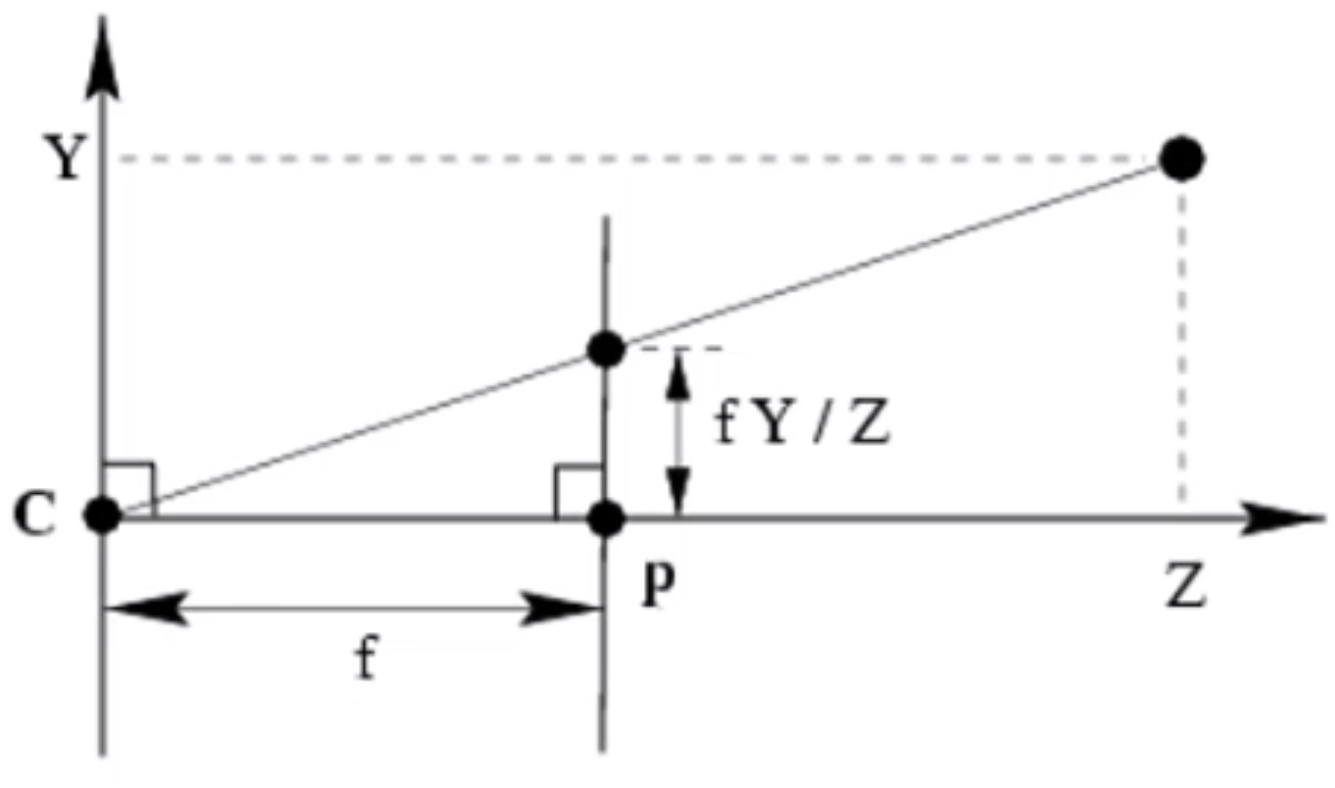
\includegraphics[width=0.5\textwidth]{figures/pinhole_sideview.png}
\caption{Pinhole sideview used in intrisic parameter estimation}
\label{fig:pinhole_sideview}
\end{figure} 

From similar triangles between the scene point and the image point, we can estimate the image point.
\begin{equation}
	x_{im} = \begin{bmatrix}
	u \\
	v \\
	1
\end{bmatrix} = \begin{bmatrix}
f \frac{x_s}{z_s}  \\
f \frac{y_s}{z_s} \\
1
\end{bmatrix} 
\end{equation}
and converting to homogeneous coordinates using the projection matrix $ P $:
 \begin{equation}
\begin{bmatrix}
u \\
v \\
w
\end{bmatrix} = \begin{bmatrix}
f & 0 & 0 & 0 \\
0 & f & 0 & 0 \\
0 & 0 & 1 & 0
\end{bmatrix} \begin{bmatrix}
x_s \\
y_s \\
z_s \\
1
\end{bmatrix} 
\end{equation}

$ f $ is the focal length.


Thus the intrinsic paramers are:
 \begin{equation}
\begin{bmatrix}
u' \\
v' \\
w'
\end{bmatrix} = \begin{bmatrix}
\alpha_x  & s & x_0 & 0 \\
0 & \alpha_y & y_0 & 0 \\
0 & 0 & 1 & 0
\end{bmatrix} \begin{bmatrix}
x_s \\
y_s \\
z_s \\
1
\end{bmatrix} 
\end{equation}
where 
\begin{itemize}
	\item $ \alpha_x, \alpha_y $ "focal length" measured in pixels
	\item $ x_0, y_0 $ coordinates of image center
	\item $ s $ skew parameter for non-orthogonal axis (usually $ 0 $)
	\item $ u', v', w' $ homogeneous image coordinates
	\item $ x_s, y_s, z_s $ scene points in camera coordinate system.
\end{itemize}


The extrinsic parameters are then:
\begin{equation}
P = \begin{bmatrix}
\alpha_x  & s & x_0 & 0 \\
0 & \alpha_y & y_0 & 0 \\
0 & 0 & 1 & 0
\end{bmatrix} \begin{bmatrix}
R & T \\
0_3^{T}  & 1
\end{bmatrix}
\end{equation}
Which projects any coordinate from the world onto the image frame. 

\begin{figure}[H]
\centering
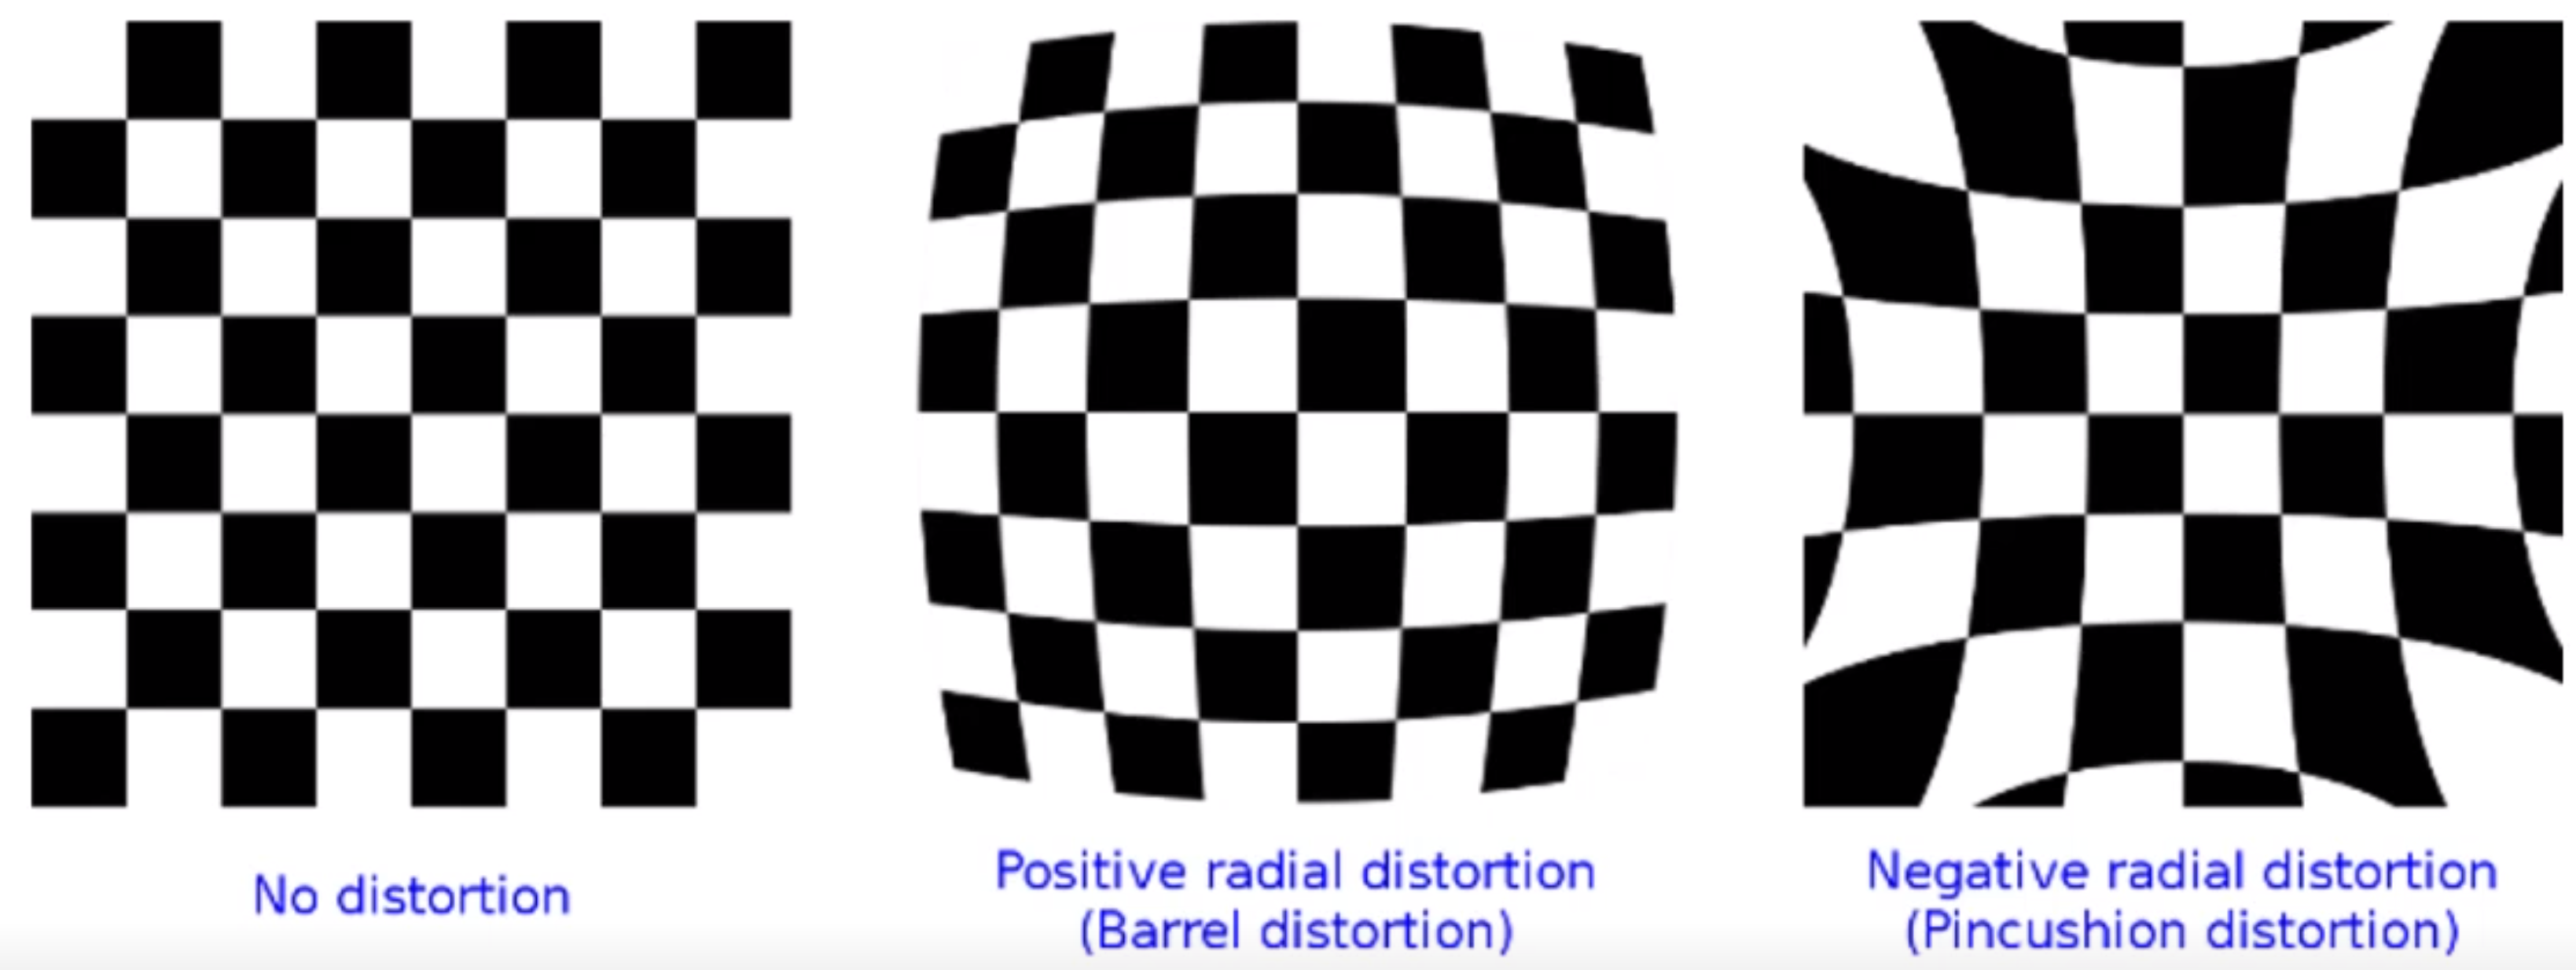
\includegraphics[width=0.9\textwidth]{figures/Radial_distortion.png}
\caption{Radial distortion}
\label{fig:radial_distortion}
\end{figure} 

\subsubsection*{Camera calibration in practice}
Using a bunch of images of a checkerboard:
\begin{enumerate}
	\item Find edges
	\item Perform straight line fitting
	\item Intersecting lines to find corners
	\item Normalize image + space points
	\item Use Linear transformation
	\item Find solution + error
	\item Adjust parameters and reiterate
\end{enumerate}


\subsubsection{Hand-eye calibration}
It is important to know the mapping between the camera on the end effector and the flange. If this transformation is not known, we see failures to grasp stuff, and collisions with the environment. 
\subsubsection*{Eye-on-hand}
The camera is positioned on the end-effector.
\begin{figure}[H]
\centering
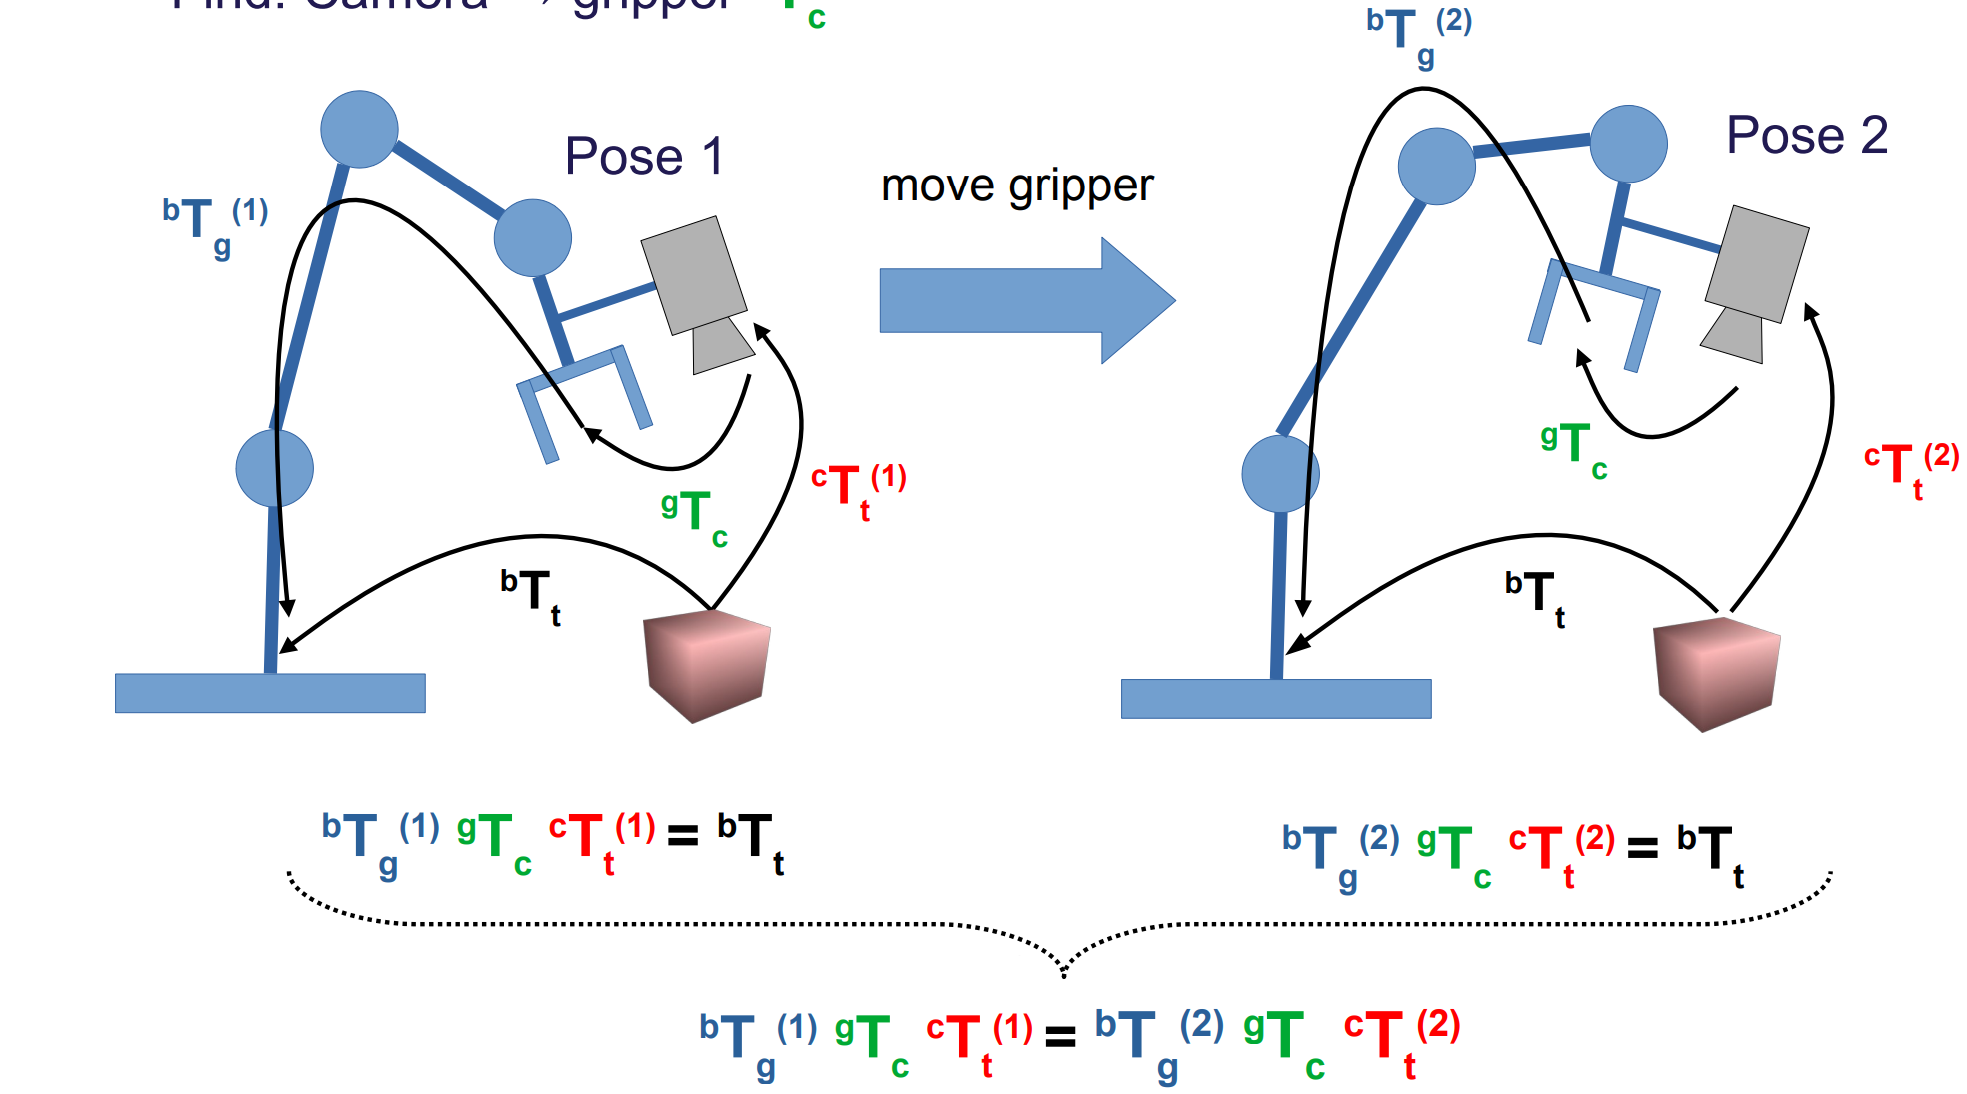
\includegraphics[width=0.8\textwidth]{figures/eye_on_hand.png}
\caption{Eye on hand calibration}
\label{fig:eye_on_hand}
\end{figure} 

we want to find the transformation from the gripper to the camera. \\
Use the red transformation from the camera to the target, but this may be unknown, so we can use a checkerboard as a target. 
We isolate the types of transformations such that $ AX = XB $
\begin{itemize}
	\item $ X $ camera $ \rightarrow $ gripper (unknown)
	\item $ A $ gripper $ \rightarrow $ base (forward kinematics)
	\item $ B $ target $ \rightarrow $ gripper (checkerboard)
\end{itemize}
This equation can be solved for $ X $ using the OpenCV function \textit{calibrateHandEye()} 
\textbf{Important:} the checkerboard must stay fixed during calibration. It is only relative transformations, not absolute. 

\subsubsection*{Eye-on-base}
Camera relative to base. 
Mount the checkerboard on the end-effector, and the camera on somewhere else. 
The idea is the same. 

% -----------------------------------------------------------------------------------------------------------------------
\newpage
\centering
\section{Pool}
\raggedright
\newpage
\subsection{Clustering algorithms}
Unsupervised learning.

\subsubsection*{Note on fitting}
For sparse datasets it is a good idea to use cross validation, where the model is trained on e.g. 4/5 parts of the data, and validated across the last 1/5. Then during the test phase, no additional tweaks to the hyper paramereters are permitted. 
\begin{figure}[H]
\centering
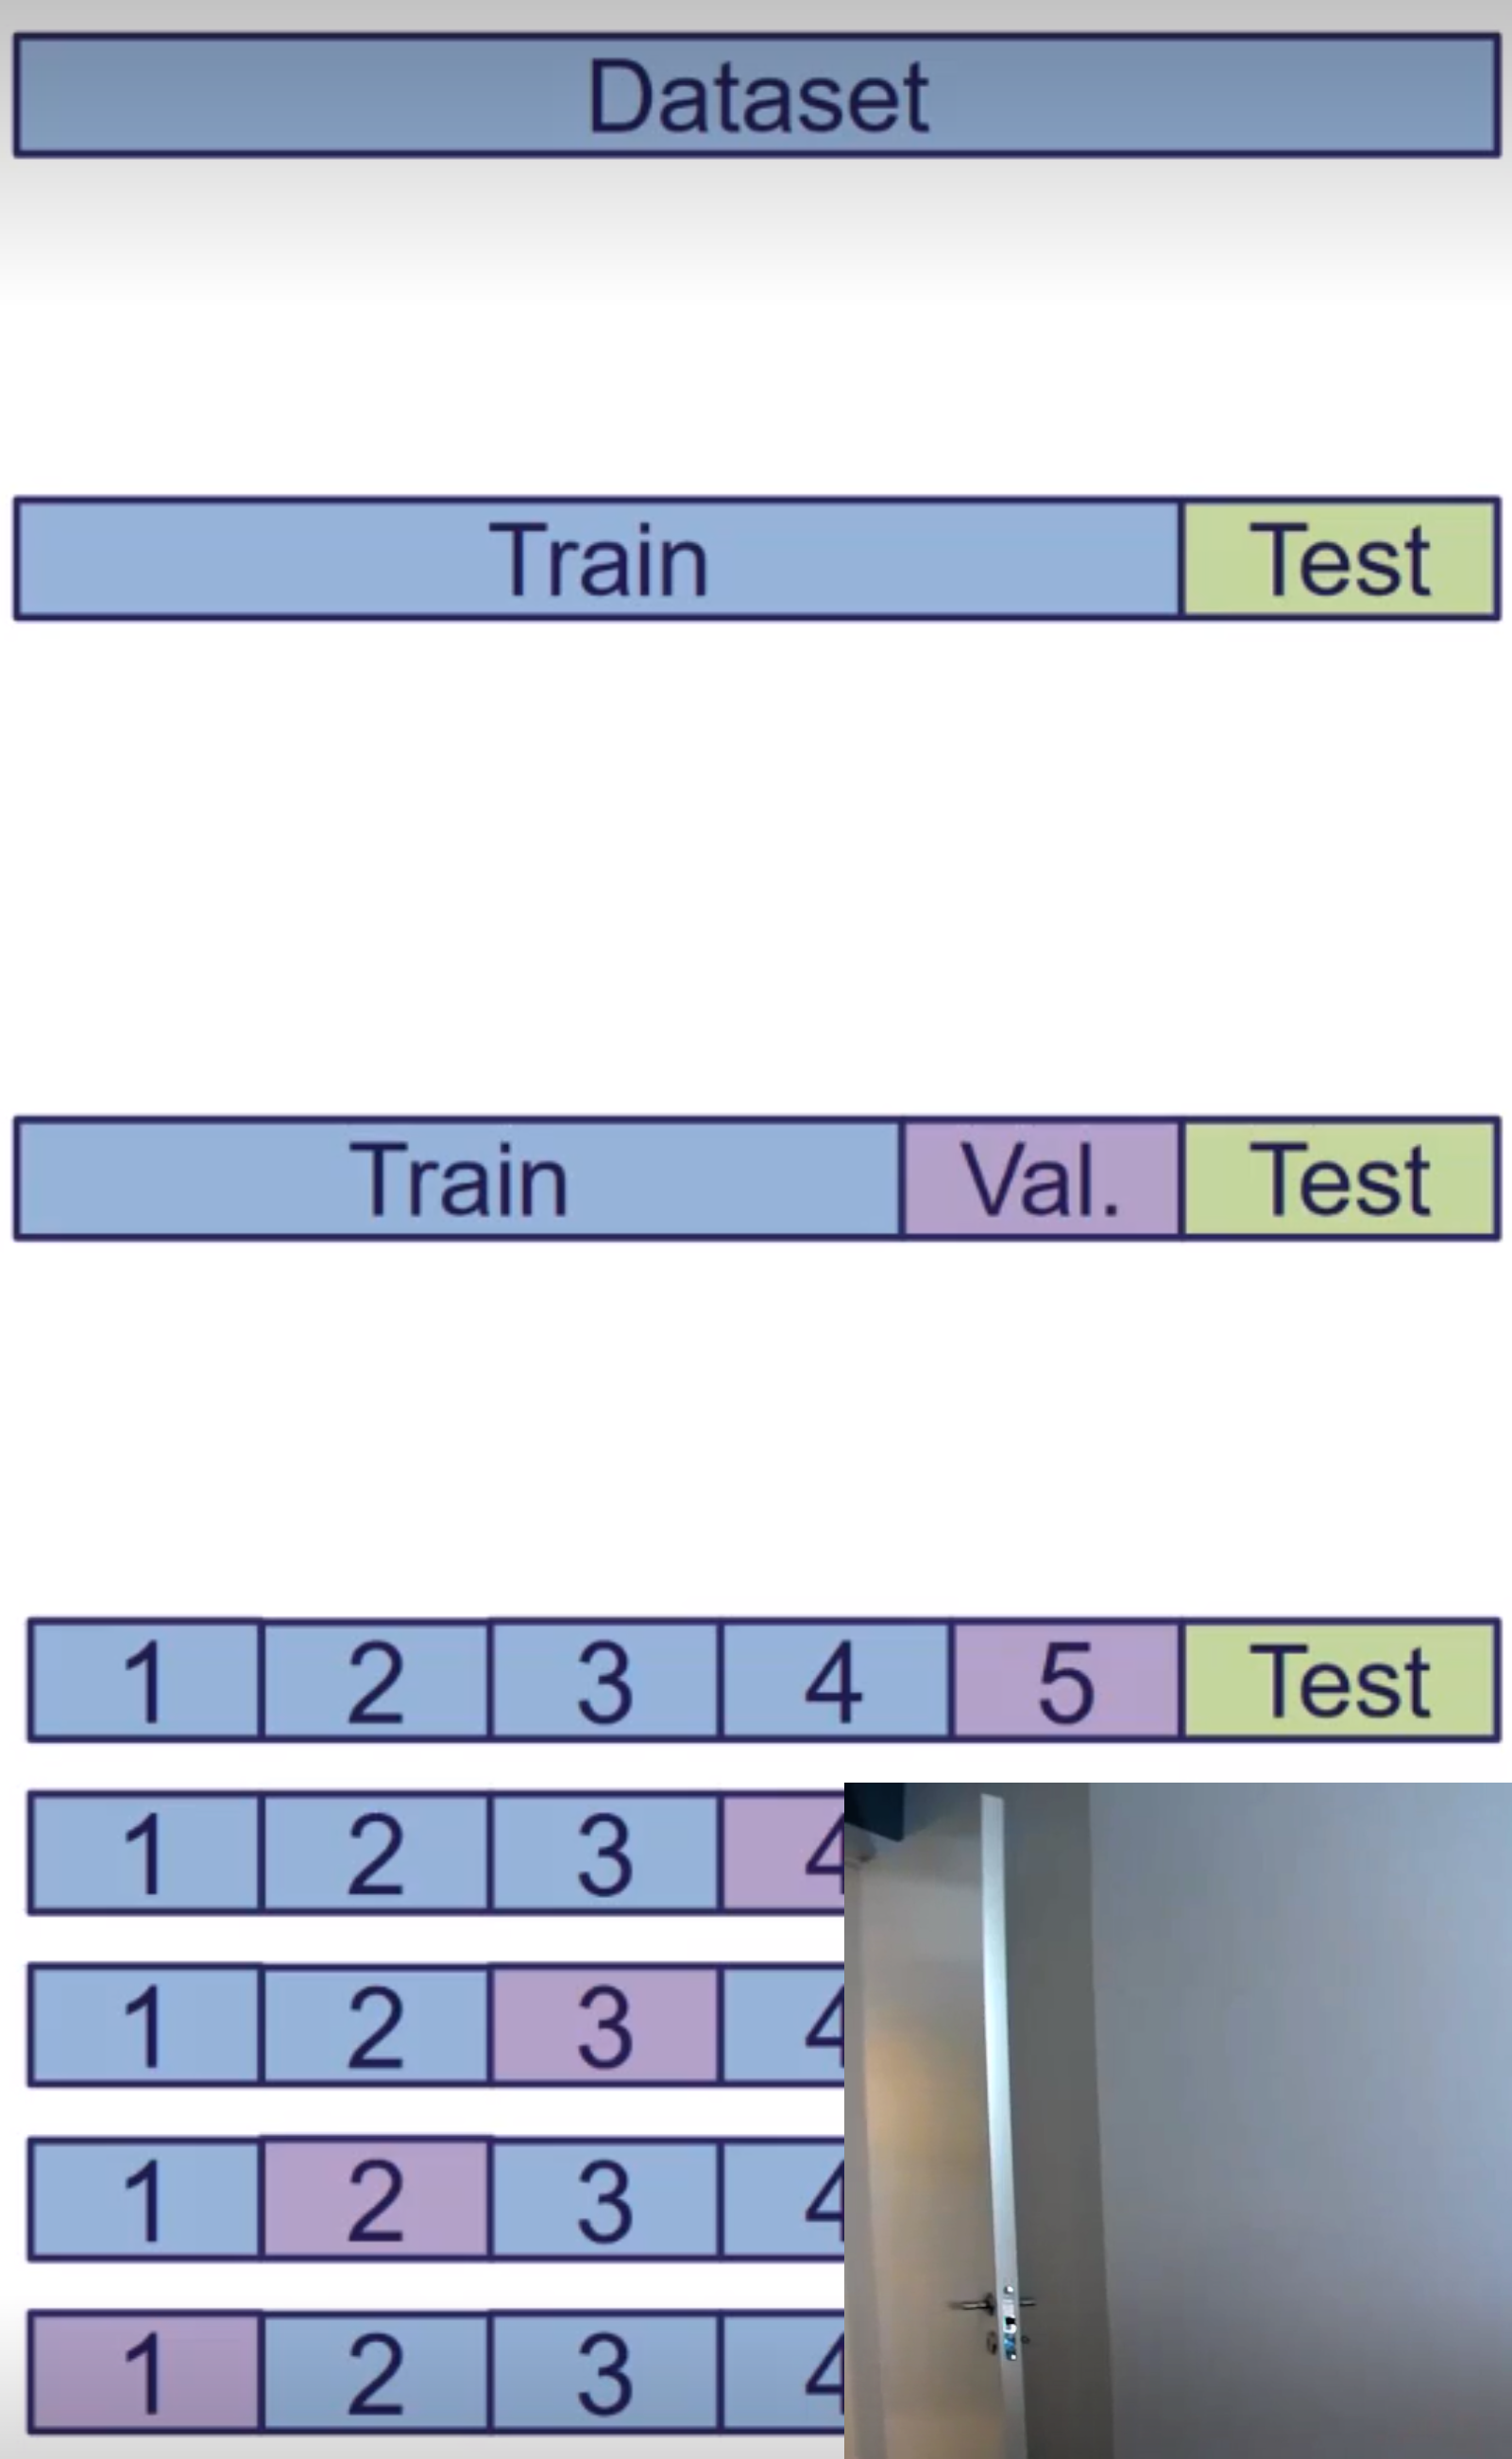
\includegraphics[width=0.5\textwidth]{figures/Train_val_test.png}
\caption{Splitting the dataset into test, validation and training set.}
\label{fig:train_val_test}
\end{figure} 

\subsubsection*{Note on Performance}
\begin{itemize}
	\item \textbf{Precision}  $ \rightarrow $ Measure of positive prediction values $ P = \frac{TP}{TP + FP} $ 
	\item \textbf{Recall}  $ \rightarrow $ Measure of sensitivity $ R = \frac{TP}{TP + FN}  $
\end{itemize}

\textbf{ROC - Reciever operating curves:} 
A graph displaying the FP to TP ratio (The further up in the left corner, the better. )

\textbf{Precision-recall curves:} 
A curve displaying the recall (horizontal axis) compared to the precision (vertical axis)

\subsubsection{K-means clustering}
Assuming that points of the same group are in close proximity of each other. 

\textbf{Algorithm} 
\begin{enumerate}
	\item Randomly \textbf{initialize} $ k $ cluster centers.
	\item Compute the \textbf{distance} between points and all the centers. 
	\item \textbf{Assign}  each point to the closest center. 
	\item \textbf{Update cluster centers:} average of cluster points in a group
	\item \textbf{Repeat} until \textbf{convergence}  
\end{enumerate}

can be used on featurevectors, or pixel values directly.

\textbf{Problems:} 
\begin{itemize}
	\item If a cluster is confined within another cluster, it will assign the datapoints to the outer cluster. I.e. it cannot differ. 
	\item You must choose $ k $
	\item Sensitive to \textbf{outliers} 
	\item Local minima in the \textit{within-cluster squared error} cost function may exist. 
	\item Detects only spherical clusters
\end{itemize}

\subsubsection{Mean-shift clustering}
Based on mean shift tracking \\
\textbf{Pros:} does not need predefined number of clusters. \\
\textbf{Cons:} need to choose windowsize/radius. 

Start with a grid of centers, and then let run the algorithm and let the grid points converge towards the center of mass in each iteration. Lastly overlaps are removed, such that there is only the corrent number of clusters left. 


\subsubsection{DBSCAN - Density-based Spatial Clustering of Applications with Noise}
Works by connecting close points within some distance from each other. It also focusses on defining core points with the most neighbors. They are chosen based on a threshold, such that they must have mroe than minPts neighbors to be considered a core point. Neighboring core points along with their respecitve non core points are added to the the cluster.

\textbf{Algorithm:} 
\begin{enumerate}
	\item Compute neighbors within $ \epsilon $ distance of each point and identify core points with more than minPts neighbors
	\item Join neighboring core points into clusters
	\item For each non-core point do:
		\begin{itemize}
			\item Add to a neighboring core point if possible
			\item Otherwise add to noise
		\end{itemize}
\end{enumerate}

This algorithm can handle noise well, and has no limitations of shapes on the clusters. but you need to choose $ \epsilon $and minPts. 

\begin{figure}[H]
\centering
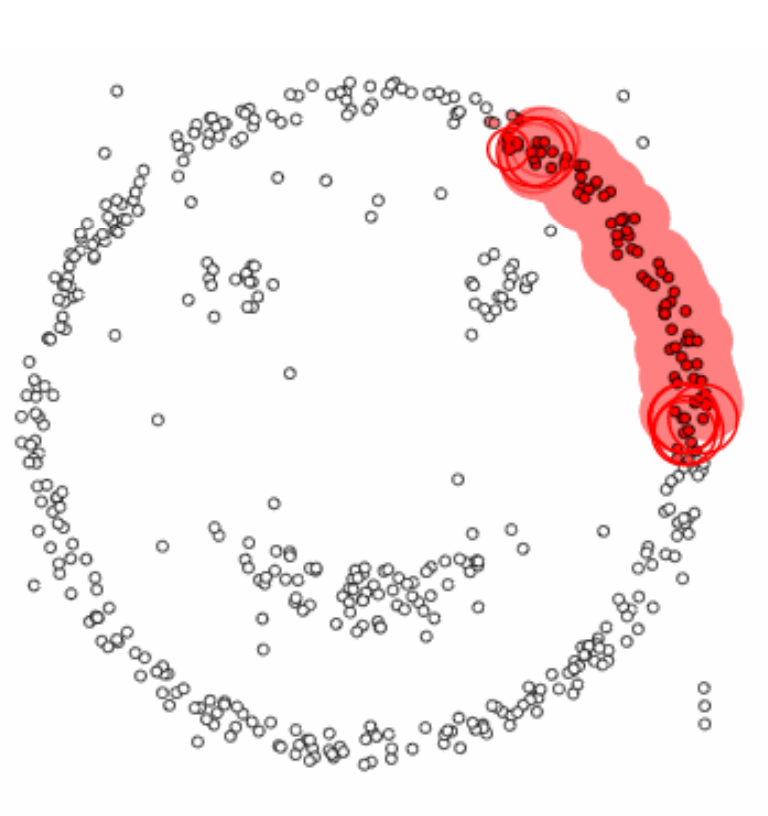
\includegraphics[width=0.5\textwidth]{figures/DBSCSAN.png}
\caption{Illustration of clustering with DBSCAN.}
\label{fig:DBSCAN}
\end{figure} 

% -----------------------------------------------------------------------------------------------------------------------
\newpage
\subsection{Classification algorithms}
You can use partitions, which is splitting single variables e.g. features, into two or more partitions. This could be done using thresholds. 

\subsubsection{Decision tree classifiers}
Using partitions in the featurespace, we can use trees to decide wether or not a particular datapoint should be in partition x. So when we get new data in, then we will be able to decide which partition it resides in. But there may be outliers, therefore we can use the probability of the sample being in partition x, and choose the highest probable partition. 


The tree is determined by training, by starting with all the features in the root node. Then every possible binary split is computed. For each split, then entropy and thereby information gain is computed. The highest information gain is chosen for that node. If a node ends up having only one features belonging to one class, it is left as a leaf node, and thereby we are sure that there is no more splits needed. 

\begin{figure}[H]
\centering
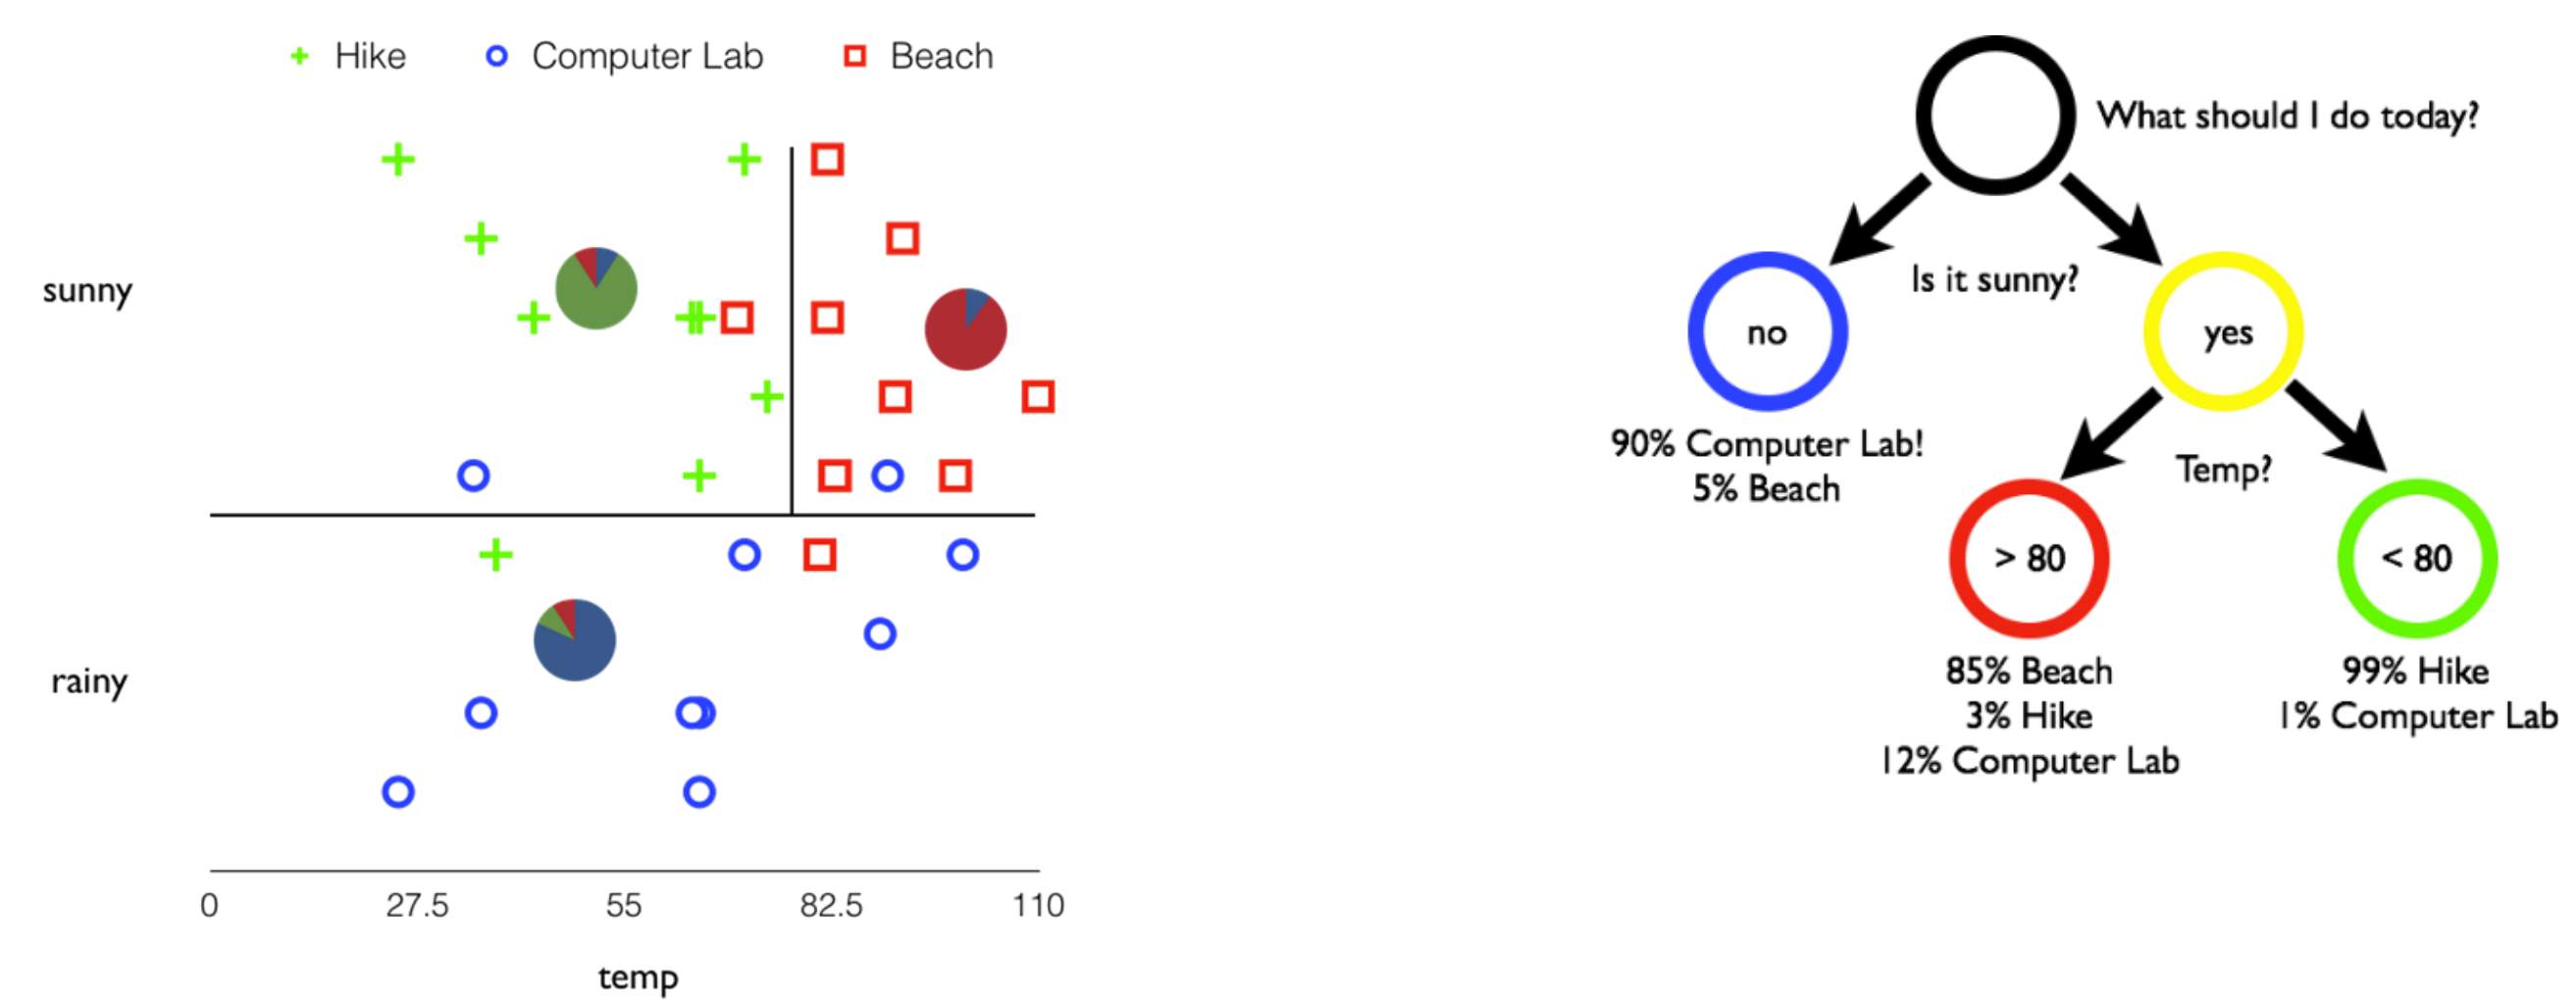
\includegraphics[width=0.99\textwidth]{figures/Decision_trees.png}
\caption{Decision tree example}
\label{fig:Decision_tree}
\end{figure} 

\subsubsection{Random Forest}
It creates multiple decision trees.\\
When a new datapoint needs to be classified, it is run through all the decision trees, which each gives their own independent classification. Then we use \textbf{majority voting} by choosing the class which constituted the highest number of classifications. 

Based on a labelled training set of $ N $ cases.

\textbf{Algorithm} 
\begin{enumerate}
	\item If the number of cases in the set is $ N $, sample $ N $ cases at random $ \rightarrow $ with replacement. This sample is used to grow the tree. 
	\item If there are $ M $ input features, a number $ m << M $ is specified at each node. $ m $ variables are selected, at random out of the $ M $ features, and the best split on these $ m $ is used to split the node. $ m $ is constant throughout the forest growing. 
	\item Each tree is grown to the largest extent possible. No branches are removed (no pruning)
	\item Predict new data by aggregating (grouping) the predictions of the $ n $ trees, and use majority voting to classify. Use the average for regression problems.
\end{enumerate}


\begin{figure}[H]
\centering
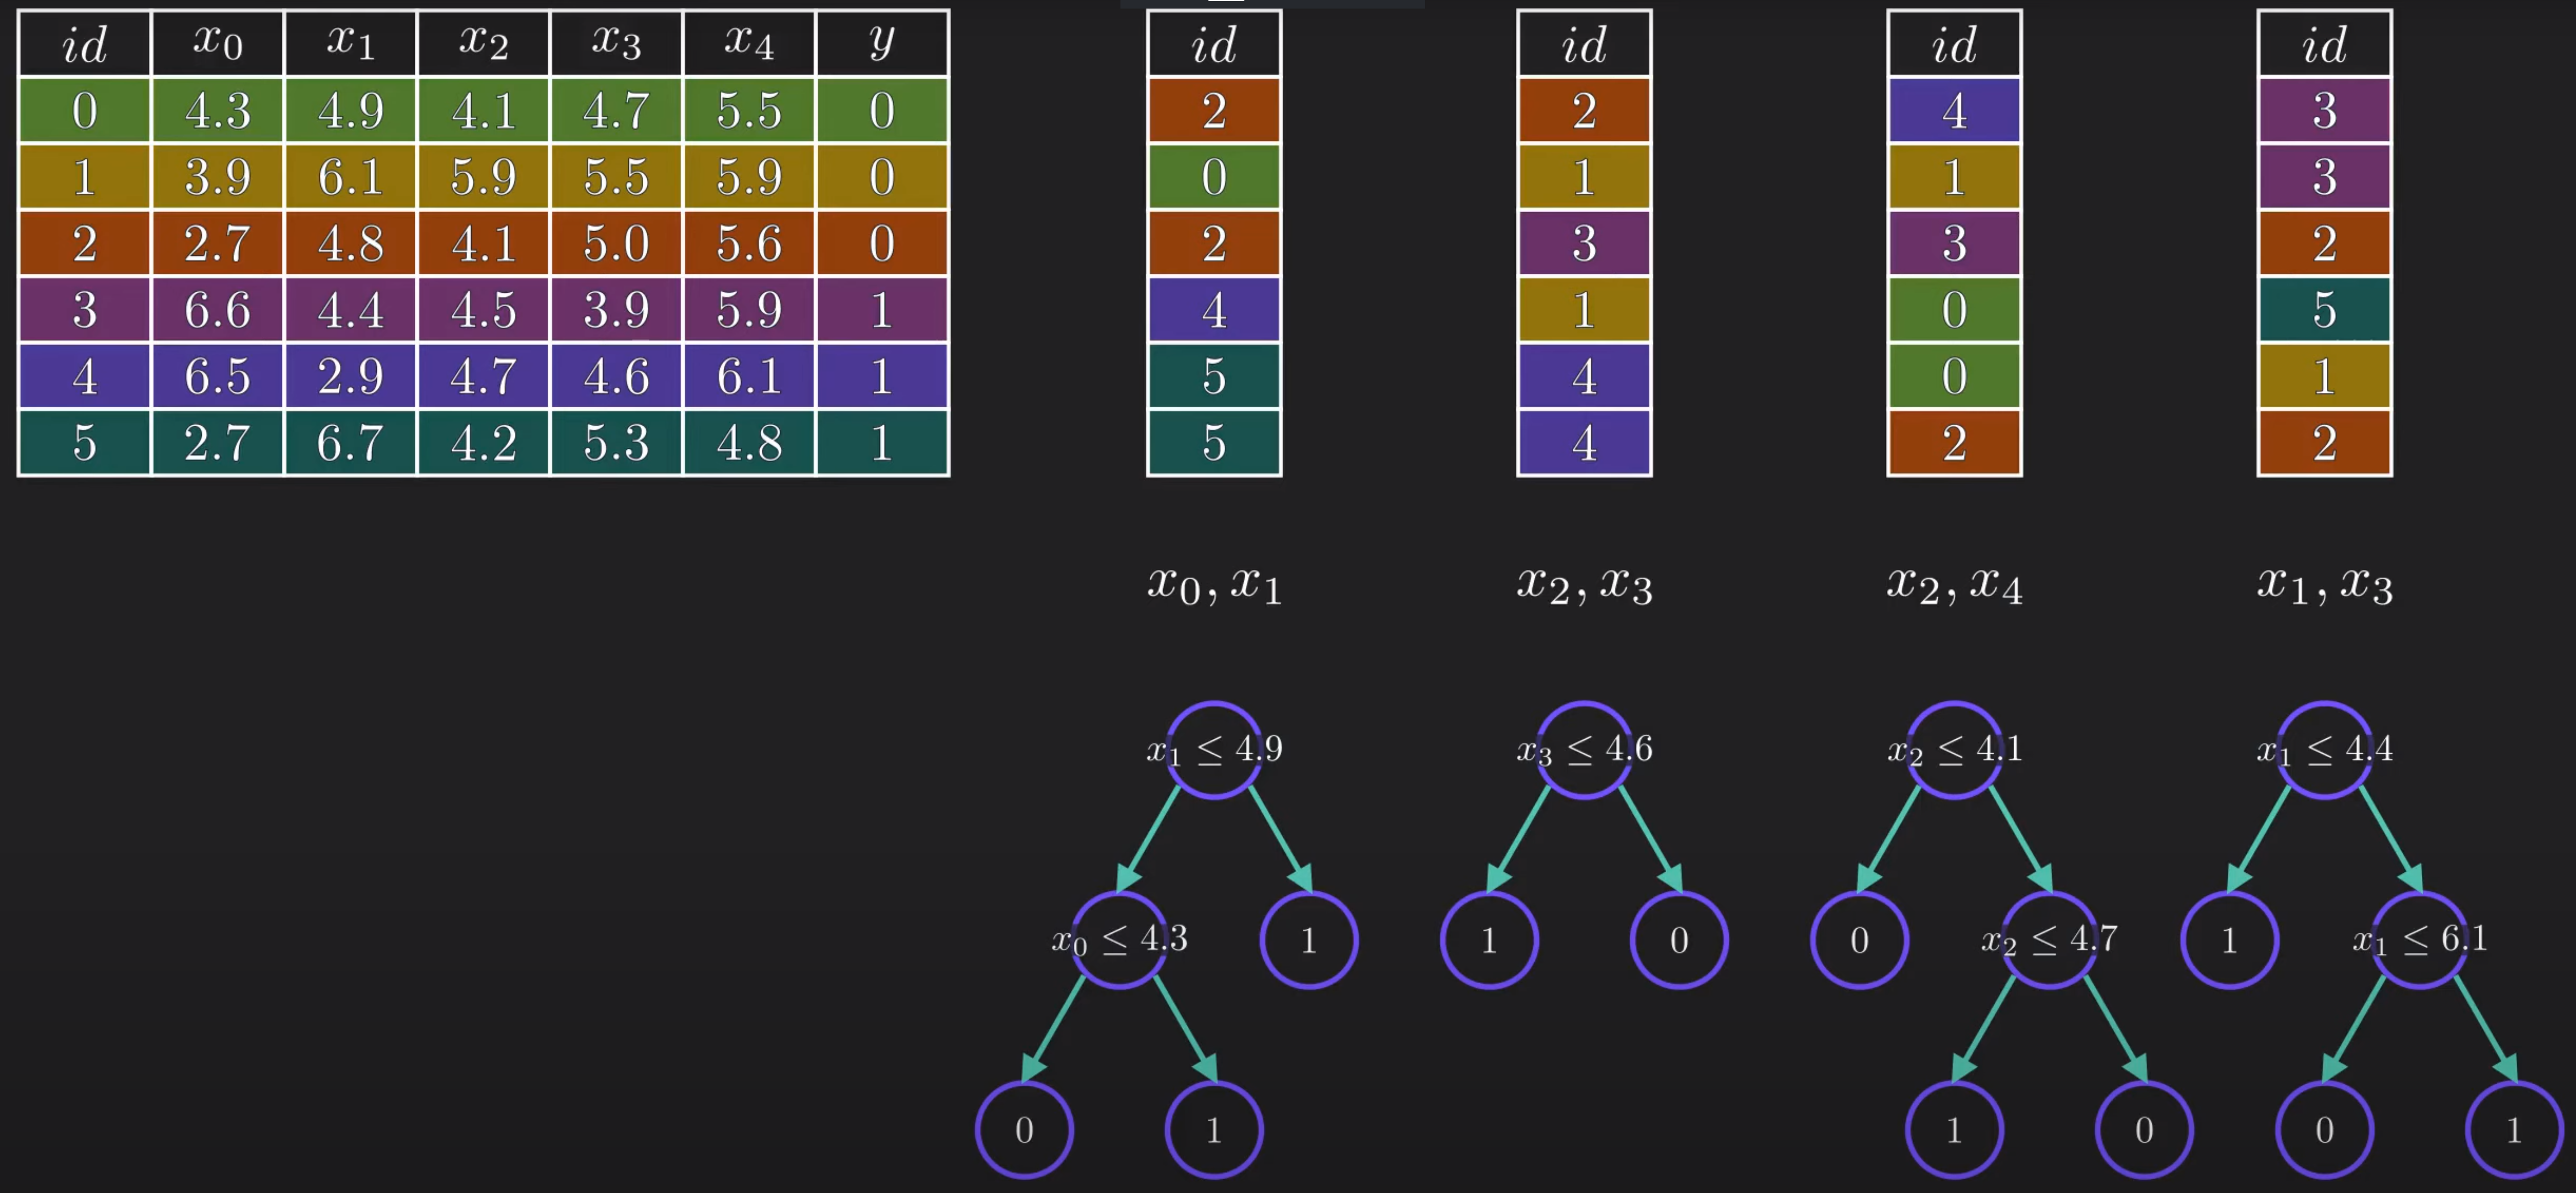
\includegraphics[width=0.9\textwidth]{figures/Random_forest.png}
\caption{Random Forest algorithm}
\label{fig:random_forest}
\end{figure} 



\subsubsection{SVM - Support Vector Machines}
Using hyperplanes to seperate datapoints. It tries to \textbf{maximize margin} towards the nearest datapoints. \\
For linear case, it is called linear SVM. \\ 
For every chosen line, increase the margin until a datapoint is reached. The reached datapoint is called \textbf{support vectors}. \\
designed for \textbf{binary} classifiers, but can be combined to solve multi-class problems.  

\begin{figure}[H]
\centering
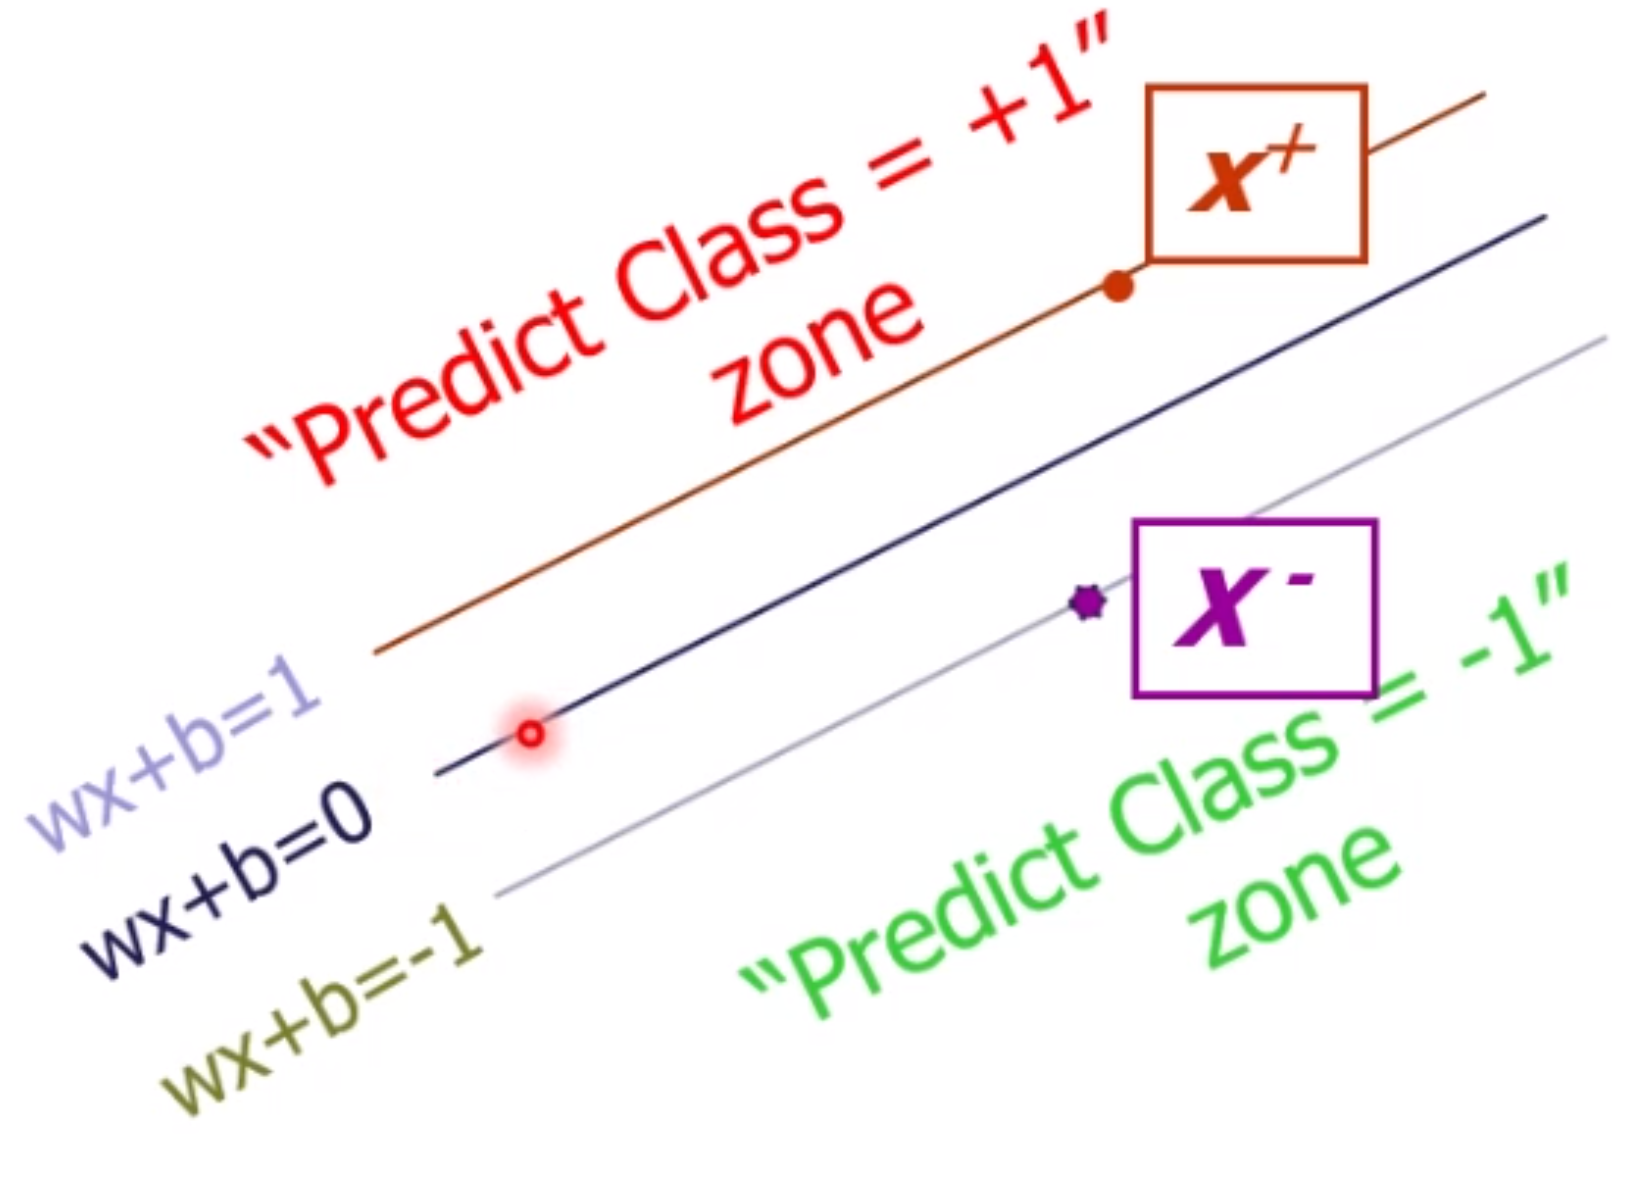
\includegraphics[width=0.4\textwidth]{figures/SVM.png}
\caption{SVM }
\label{fig:}
\end{figure} 
We label every datapoint beneath the line -1 and +1 for datapoints above. 

We compute the margin by:
\begin{equation}
M = \frac{(x^{+} - x^{-}  )w}{|w|} = \frac{2}{|w|}   
\end{equation}
Where $ w $ is the vector from the center to the margin line. 

We want to maximise the margin $ M $, which is the same as:
 \begin{equation}
	 minimize \hspace{5pt} \frac{1}{2} w^{T} w
\end{equation}
Which is solved with quadratic programming. Where ever datapoint $ y_i $ must satisfy:
\begin{equation}
y_i(w x_i + b) \geq 1 \forall i
\end{equation}

\textbf{noisy trainingset} $ \rightarrow $ slack variables \\

\textbf{Non-linear} case $ \rightarrow $ map to higher dimension using  \textbf{Kernel functions} .


\textbf{Proporties of SVM} 
\begin{itemize}
	\item Great with large datasets/featurespaces $ \rightarrow $ only uses support vectors
	\item Overfitting can be handled with slack variables.
	\item Convex problem $ \rightarrow $ one solution
\end{itemize}


% -----------------------------------------------------------------------------------------------------------------------
\newpage
\subsection{CNN: Convolutions, pooling}
\begin{itemize}
	\item We \textbf{learn features} instead of handcrafting them.
	\item We learn the classification.
	\item Handcrat networks instead.
\end{itemize}

A convolution could be a $ 3 \times 3 $, which is convoluted with the entire input image. 

\begin{itemize}
	\item Early convolutions comptue the more \textbf{global features} 
\end{itemize}

Each entry in the convolution kernel is a weight. This weight is learned through backpropagation.\\
The process of convoluting the input image is also known as filtering. It extracts features

\begin{figure}[H]
\centering
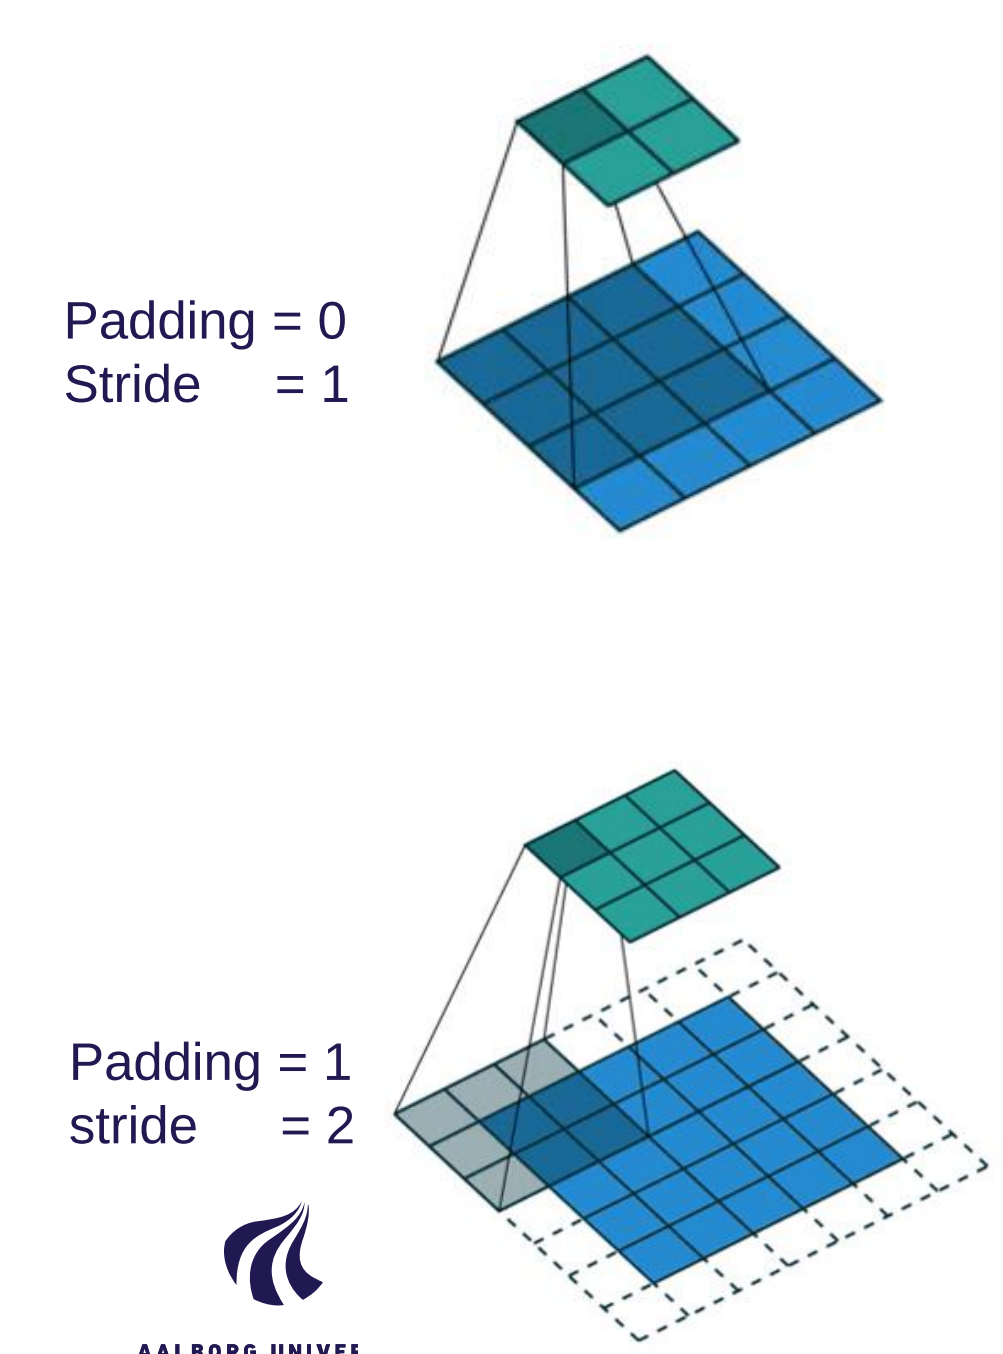
\includegraphics[width=0.6\textwidth]{figures/Stride_padding_size.png}
\caption{Illustration of filter size, padding and stride.}
\label{fig:stride_padding_size}
\end{figure} 

To preserve the size of the input feature map, then we use \textbf{padding}, which is adding $ 0  $'s to the edge. Stride is the step size.  



We stack filters into channels.
\begin{figure}[H]
\centering
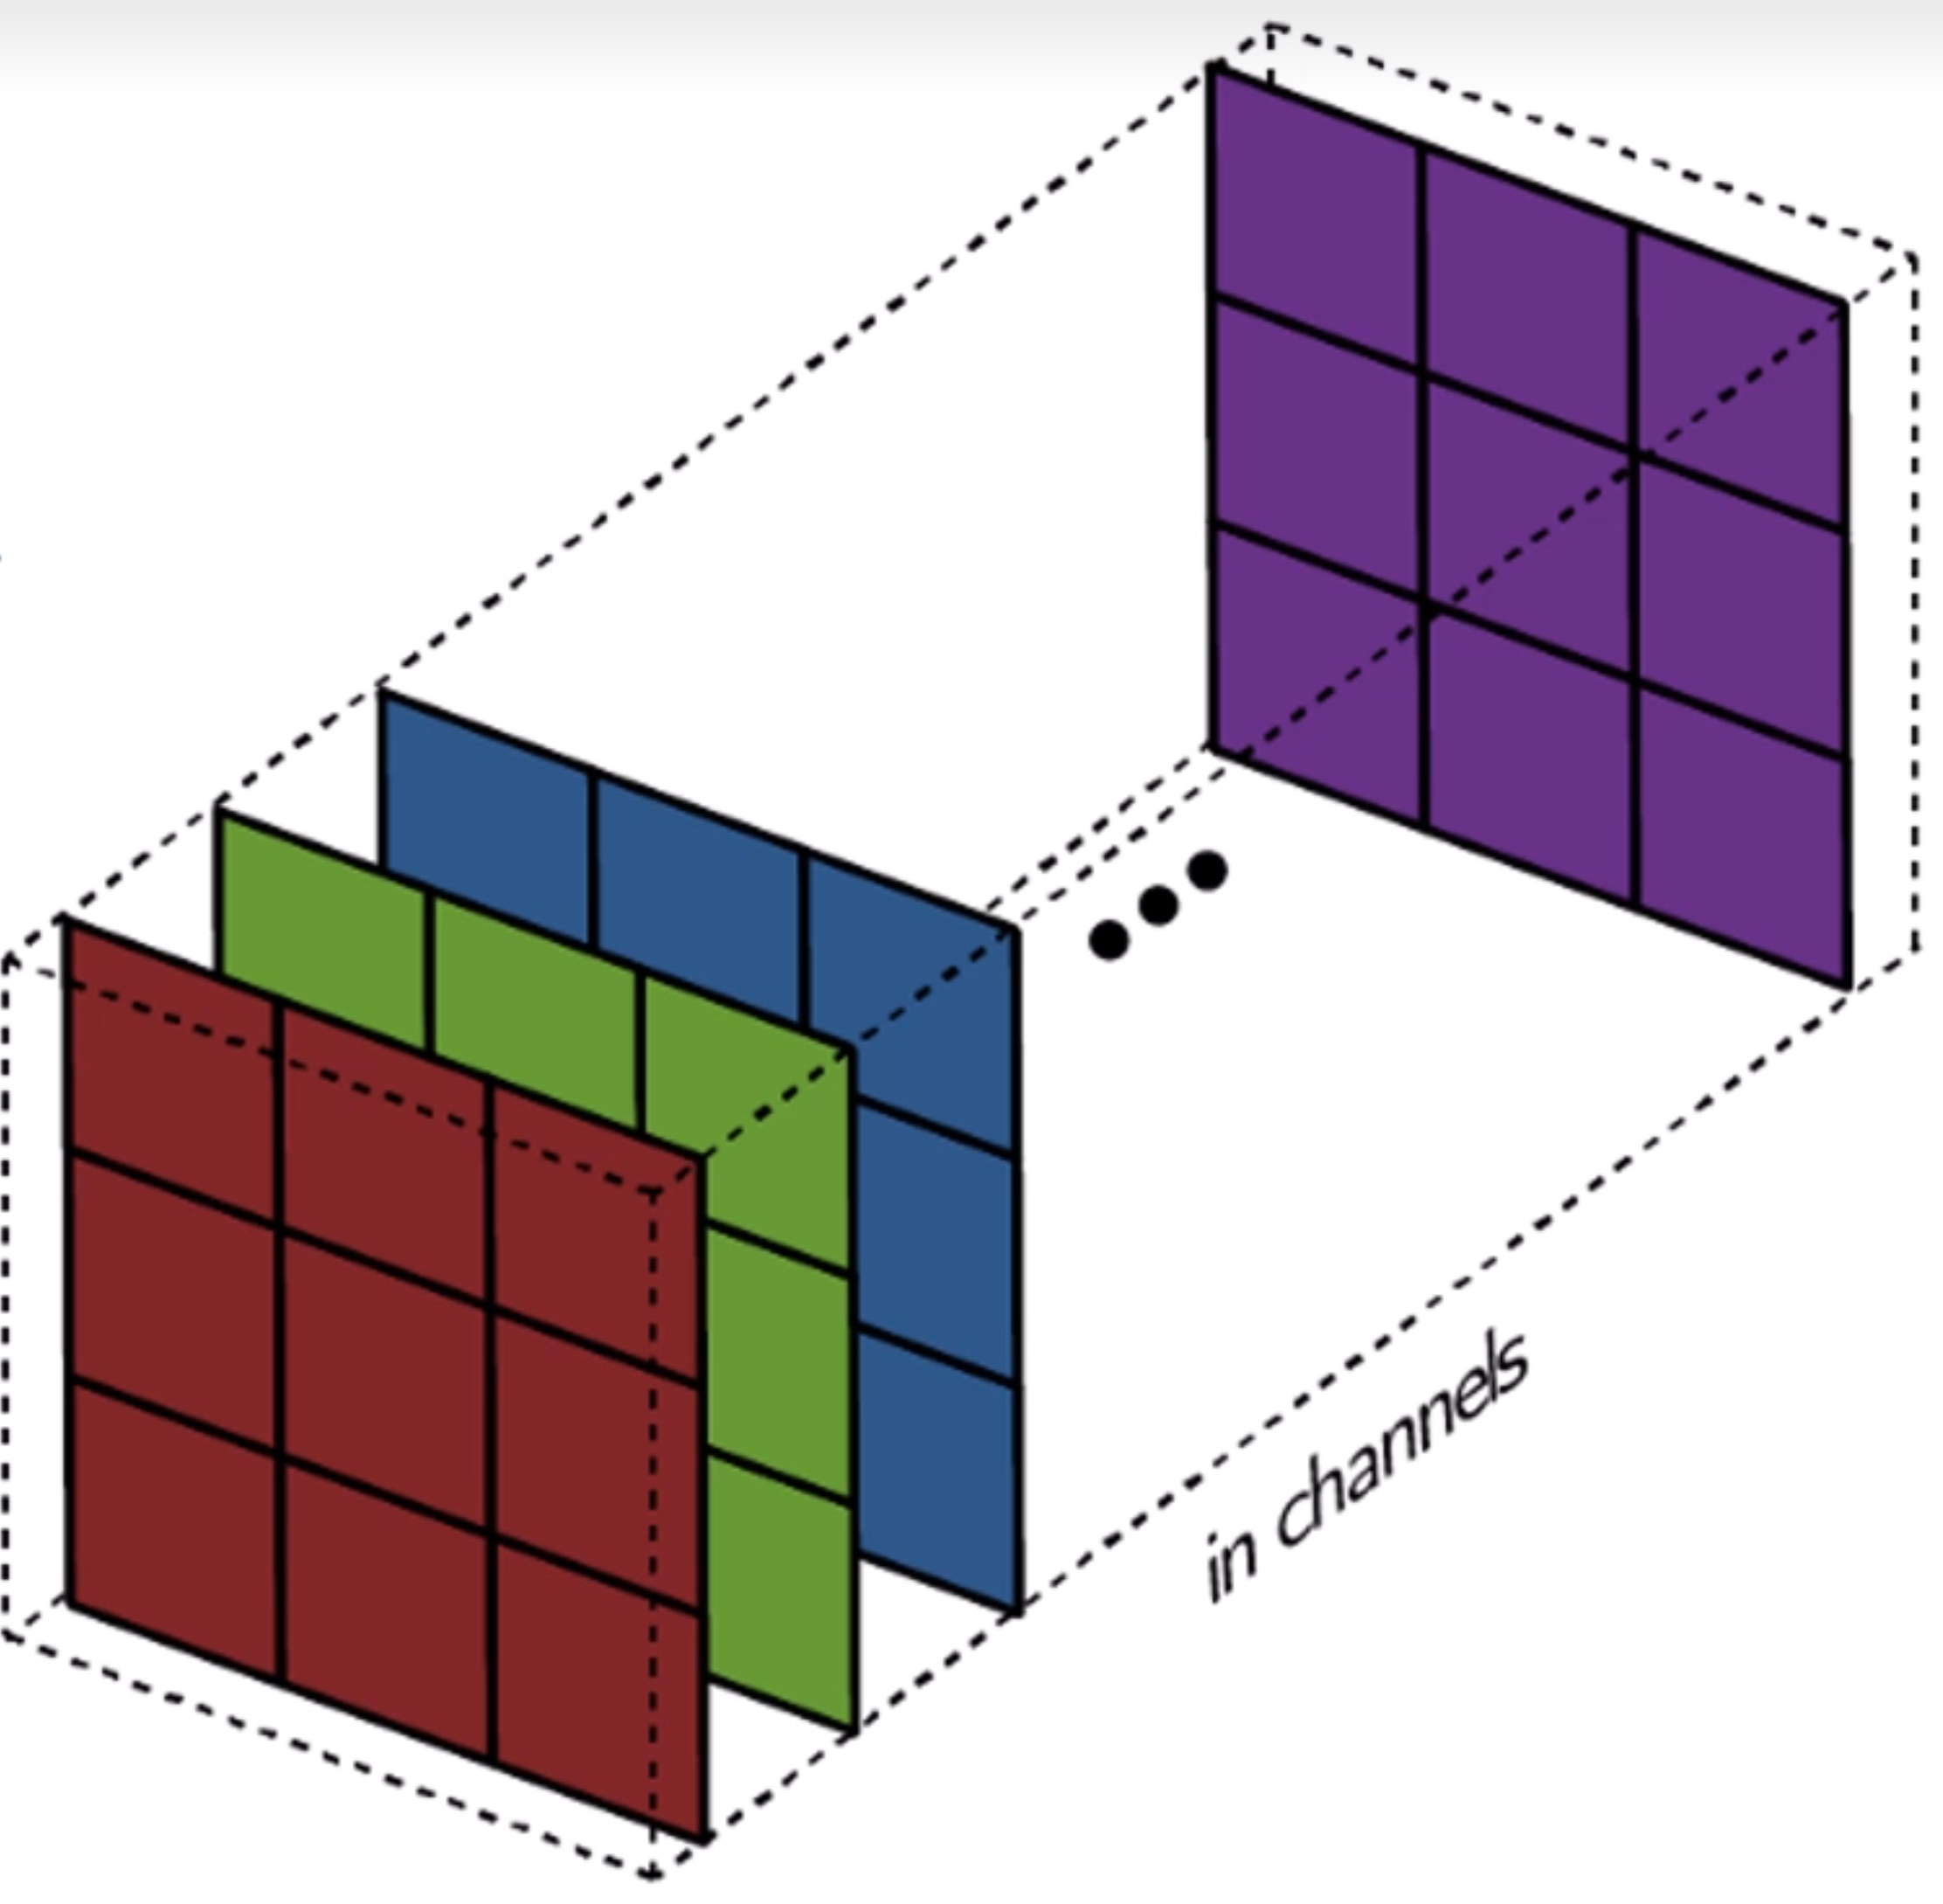
\includegraphics[width=0.6\textwidth]{figures/filter_channels.png}
\caption{Filter channels by stacking them}
\label{fig:filter_channel}
\end{figure} 


The more layers of convolutions we have, the higher level features we genererate.
\begin{figure}[H]
\centering
\includegraphics[width=0.99\textwidth]{figures/Visualizing_convolutions.png}
\caption{Different levels of details in the layers of convolutional featuremaps.}
\label{fig:visualizing_convolutions}
\end{figure} 



\subsubsection*{Stacking Convolutional layers}
\textbf{VGG-Net (2015)}\\ 
By stacking convolutional layers it is possible to \textbf{simulate a larger receptive field}. This means that for each kernel size it gets increased because we have a stride of 2. This results from a $ 3 \times 3 $ kernel, to a $ 5 \times 5 $ without having the same number of convolutional weights (parameters) that should be learned. This would be $ 2 \cdot 9 = 18 $instead of just using a standard $ 5 \times 5 $ kernel, which results in $ 25 $ parameters. 


\subsubsection*{Parallel convolutional layers}
\textbf{Inception (2015)}\\ 
By doing parallel convolutional layers, it is possible to choose in the end what layer worked the best. 

\subsubsection*{Skipping convolutional layers}
\textbf{RES-Net (2016)}\\ 
By skipping convolutional layers, it is possible to compute the residual of the featuremap, which is the difference that the actual layers does. This effectively reduces the noise in the bottom of the layer during back propagation known as the  \textbf{vanishing gradient problem}. 


\subsubsection*{Dropout}
To avoid overfitting we can use dropout. Dropout is \textbf{randomly removing 50\% of the network}, to force the network to not rely on single neurons $ \rightarrow $ Spread the knowledge out on multiple neurons. 


3 options for using a network:
\begin{itemize}
	\item Use a pretrained network
	\item Transferlearning (e.g. discarding unnecessary classes, retraining part of the weigthts by \textbf{freezing layers} , etc.)
	\item Train from scratch
\end{itemize}

\subsubsection{Pooling}
Also known as \textbf{subsampling} $ \rightarrow $ reduces the dimensions of a layer.

The types of pooling are:
\begin{itemize}
	\item MAX-pooling
	\item Average pooling
	\item Sum-pooling
\end{itemize}

Pooling is a hyperparameter, you can not learn it. 

\subsubsection*{MAX-pooling}
Most popular type of pooling. 
It finds the maximum value within the pooling kernel size, often $ 2 \times 2 $. 


\begin{figure}[H]
\centering
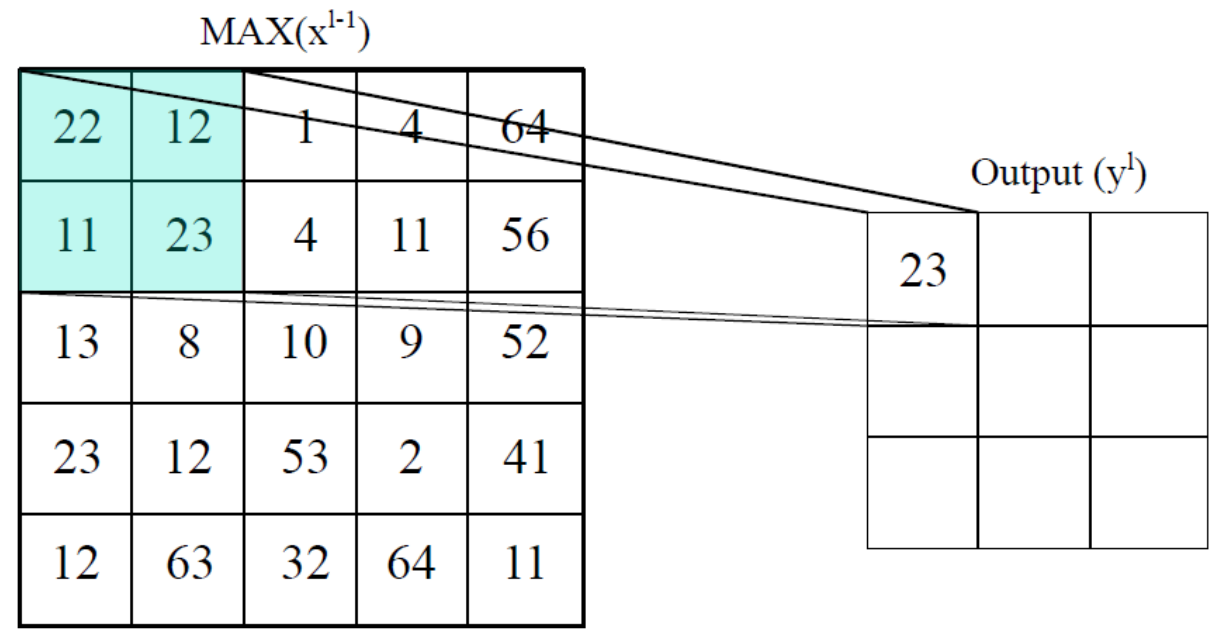
\includegraphics[width=0.8\textwidth]{figures/max_pooling.png}
\caption{Illustration of max pooling}
\label{fig:max_pooling}
\end{figure} 

% -----------------------------------------------------------------------------------------------------------------------
\newpage
\subsection{CNN: Training and fine-tuning}

\subsubsection*{Training}

The components of training CNN's are:

\begin{figure}[H]
\centering
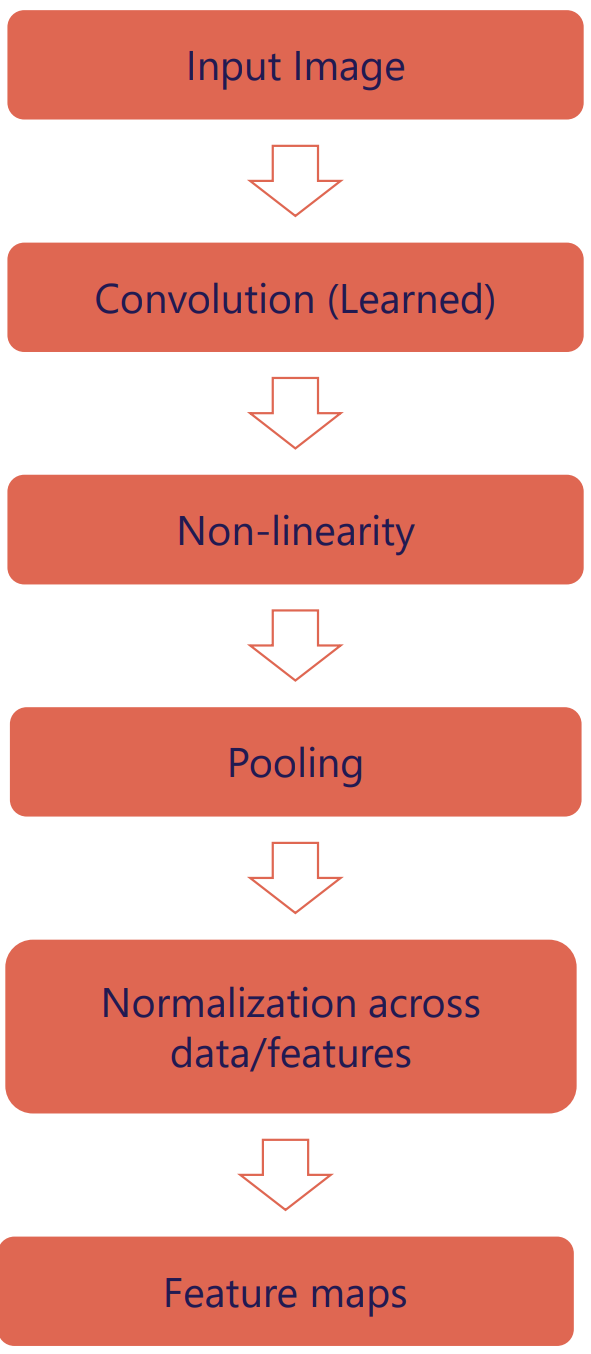
\includegraphics[width=0.2\textwidth]{figures/CNN-pipeline.png}
\caption{Components in CNN's}
\label{fig:CNN_walktrough}
\end{figure} 

This is known as feed-forward. 
\begin{enumerate}
	\item Input image
	\item Convolution: here we conduct the convolutions. They can be done multiple times to generate more featuremaps.
	\item Non-linearity: Here we apply the ReLU function which non-linearises the loos function. Done per pixel.
	\item Pooling: (optional) Here we do subsampling, by e.g. max pooling 
	\item Batch Normalization across data/features: (optional) Normalize each input for each layer and it \textbf{improves training speed, less sensitive bad initialization, and improves regularisation}. It strikes a \textbf{balance between full gradient computation and SGD}.  
	\item Fully connected layer resulting in a featuremap for classification. 
\end{enumerate}

We can have multiple convolutional layers. This is also refered to as \textbf{depth}. Width is the number of filters in that convolutional layer. 


\subsubsection*{Training steps}
\begin{enumerate}
	\item Define the problem $ \rightarrow $ \textbf{Classification / Object detection / segmentation etc.}  
	\item Collect dataset that represent the problem. $ \rightarrow $  Split into \textbf{Training, Validation, Test} 
	\item Preprocess the data $ \rightarrow $ \textbf{Normalize} or \textbf{standardize} the data  
	\item Choose the \textbf{architecture} of the network. $ \rightarrow $ Choose layers, (Convolutional, Pooling, fully connected). Specify \textbf{activation functions, input/output dimensions} 
	\item Compile the model $ \rightarrow $ Choose \textbf{Loss function, optimizer (SGD), learning rate, evaluation metrics (precision, recall etc.)}  
	\item Train the model $ \rightarrow $ Feed data through, compute loss, and update weights in back propagation. Monitor accuracy to identify potential overfitting.
	\item Tune hyper parameter tuning $ \rightarrow $ \textbf{learning rate, batch size} 
	\item Evaluate on test set.
	\item Finetune $ \rightarrow $ Adjust architecture, collect more data.
\end{enumerate}




\subsubsection*{Backpropagation}
Done using errorpropagation through the network using the chainrule. 

\textbf{Stochastic gradient descent} 
Due to the loss of gradient problem, it is necessary to use stochastic gradient descent. This is done by introducing stochastic noise into the gradients, and thus manipulating both the descent direction and the magnitude of descent.

\textbf{Momentum} 


% -----------------------------------------------------------------------------------------------------------------------
\newpage
\subsection{CNN: Object detection}

\begin{figure}[H]
\centering
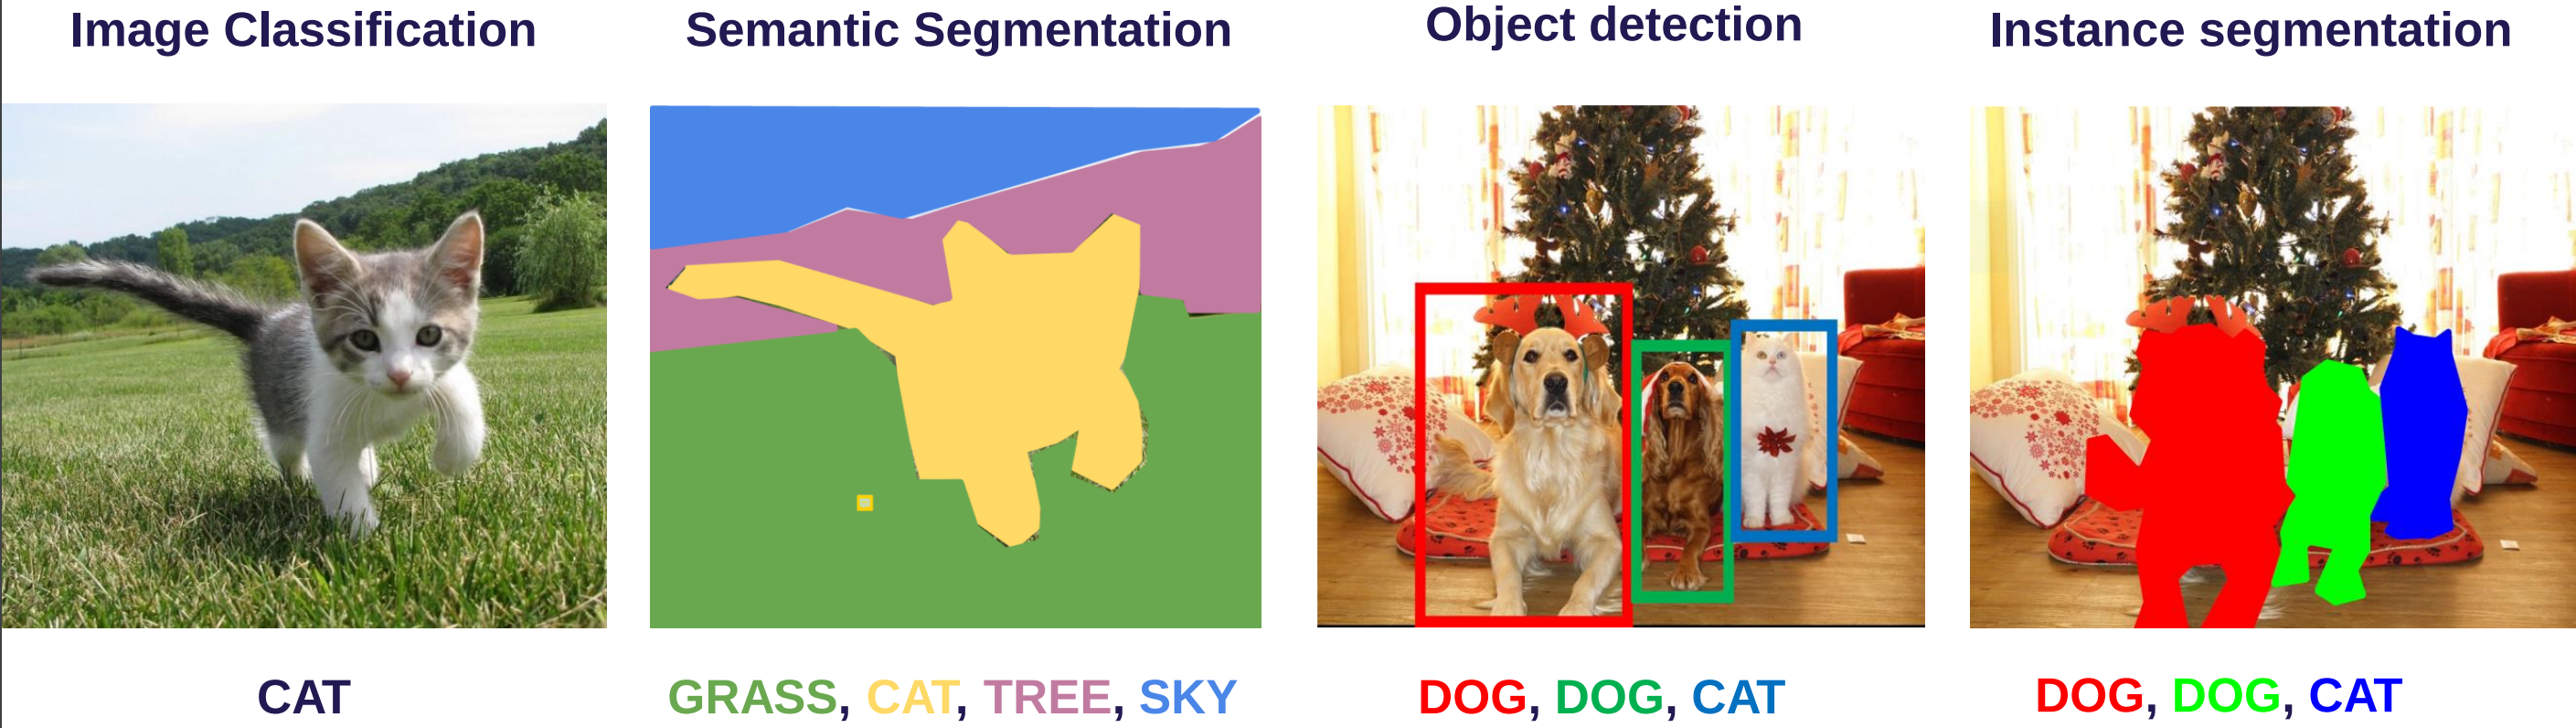
\includegraphics[width=0.99\textwidth]{figures/Types_of_CNN.png}
\caption{Different types of CNN's}
\label{fig:cnn_types}
\end{figure} 


\subsubsection*{Single Object detection}
Two tasks:
\begin{itemize}
	\item \textbf{What} is the object? 
	\item \textbf{Where} is the object? 
\end{itemize}

From the fully connected layer, we define the output layer with probabilities between 0 and 1, for each class. Compute the loss e.g. by using softmax loss. To figure out where the object is, we have a fully connected layer with regression (continuous variables) for which we compute the bounding box paramters. Here we can use the L2 loss function to figure out how far from the real bounding box it is, and by combining these two losses with a weighted sum, we get what is known as a \textbf{multitask-loss}. This is used to back propagate the CNN. 

\begin{figure}[H]
\centering
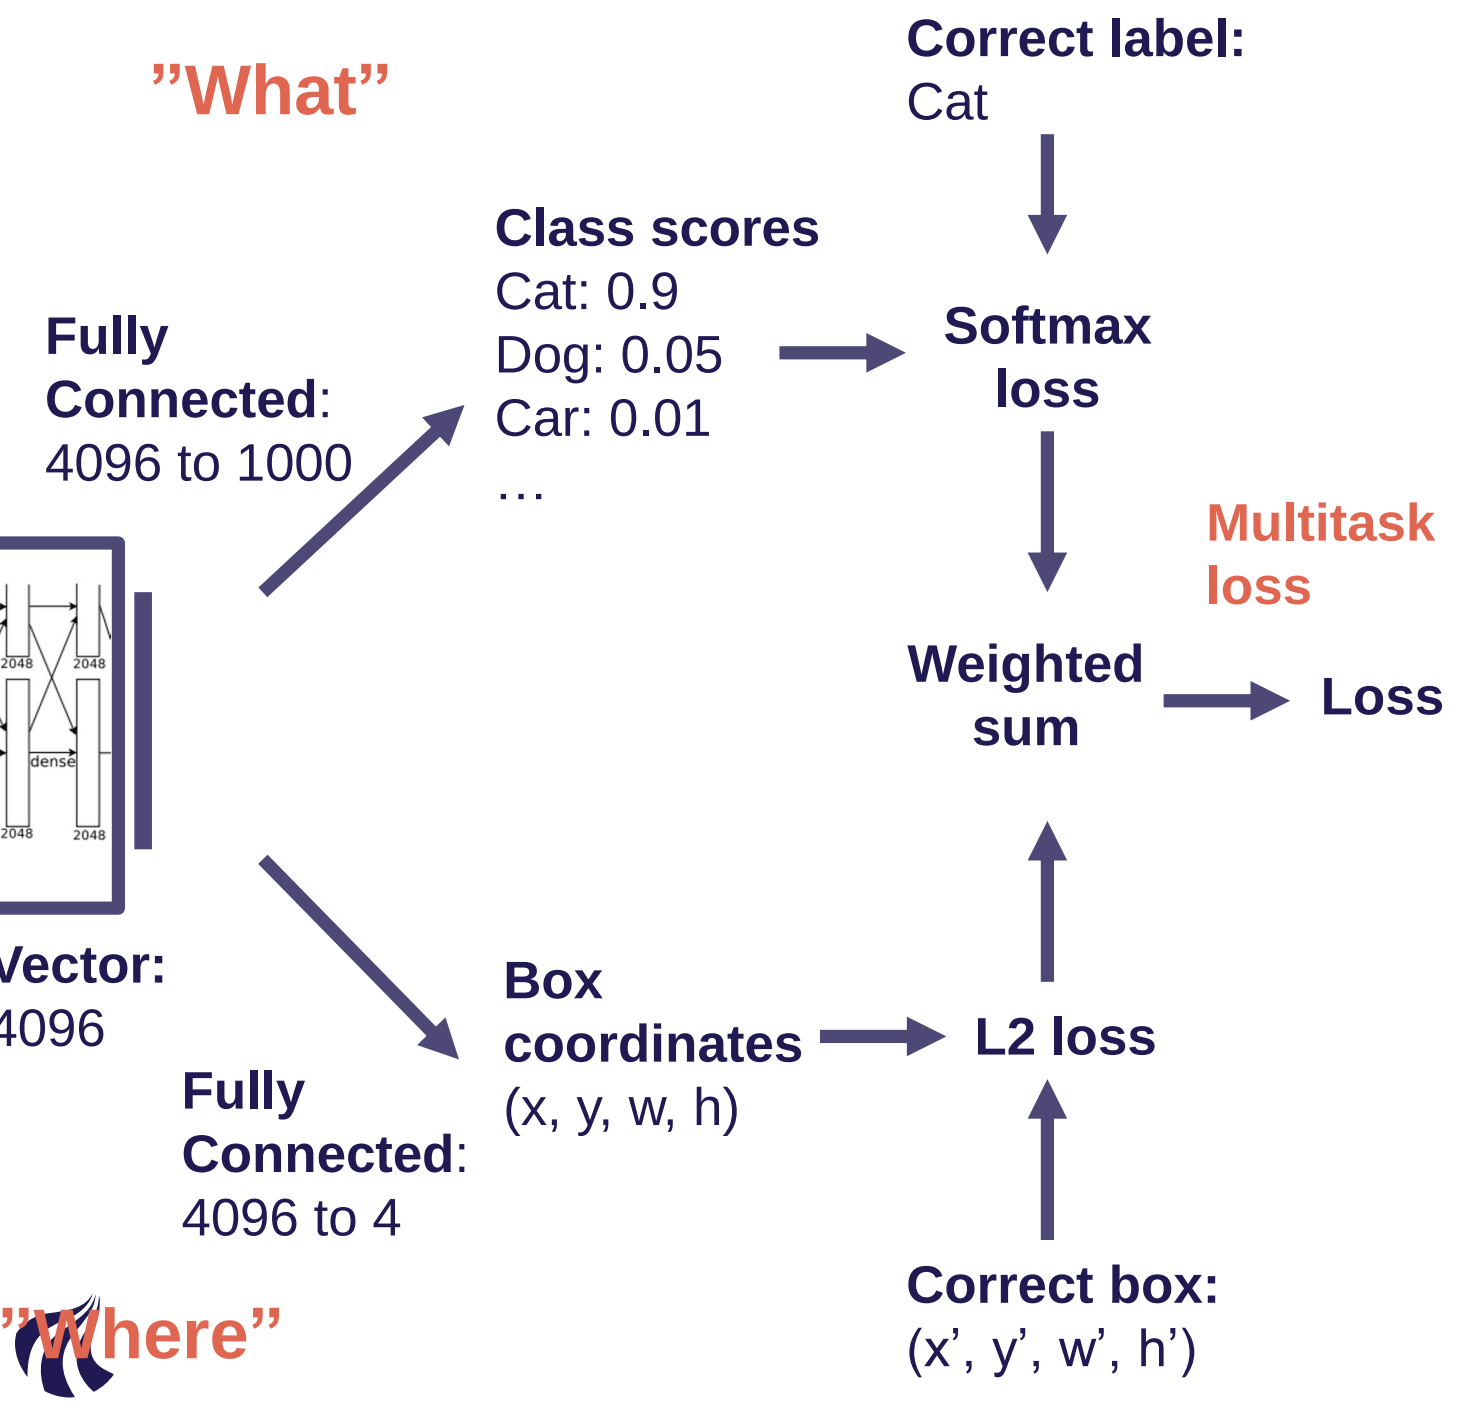
\includegraphics[width=0.7\textwidth]{figures/Single_object_detection.png}
\caption{Illustration of the head layers on single object detection.}
\label{fig:single_object_detection}
\end{figure} 


\subsubsection*{Multi Object detection}
Done by Regional-based CNN's (\textbf{R-CNN}) 

By running \textbf{Selective search} we get \textbf{region proposals}, which are boxes covering all objects.   

\begin{enumerate}
	\item Warp each region to be $ 224 \times 224 $ pixels (input size of ImageNet)
	\item Each region can be passed through a single convNet classifier network.
	\item Adjust region positons using regression.
\end{enumerate}

\textbf{Slow $ \rightarrow $ feedforward for each region} 

\vspace{15pt}


Solved by \textbf{Fast R-CNN}\\
This network takes the convolutional part and then it algins the regions, and they are cropped using \textbf{RoI Pool}. Then each region is run through a small neural network, called \textbf{per-region network}. The \textbf{seletive search} is computed on the \textbf{CPU}, so it takes a few seconds.   


\vspace{15pt}
Solved by \textbf{Faster R-CNN}\\
Here the regions are found using a CNN instead of using selective search. Known as \textbf{RPN (Regional Proposal network)}\\
We imaginge anchor boxes, for each pixel in the featuremap. Is this anchor box an object?\\

\textbf{Training the Faster R-CNN} 
\begin{enumerate}
	\item \textbf{RPN classification} Is the anchor box an object?
	\item \textbf{RPN Regression} Predict transform from anchor box to proposal box
	\item \textbf{Object Classification} Classify into backgrond /object classes
	\item \textbf{Object regression} Predict transform from proposal box to object box. 
\end{enumerate}




These are known as \textbf{Two-stage} proposals. 
There exist single stage proposals as well. These go directly to clasifying the anchor boxes instead of figuring out if the anchor box is part of an object and then figuring out what object. 


\subsubsection*{Evaluating Object detection performance}
By computing the intersection over union, we get at measure between 0 and 1 of how well the prediction fits the ground truth.
\begin{equation}
	\frac{Area of intersection}{Area of union} 
\end{equation}
\begin{itemize}
	\item IoU > 0.5 $ \rightarrow $ Decent
	\item IoU > 0.7 $ \rightarrow $ Great
	\item IoU > 0.9 $ \rightarrow $ Almost perfect
\end{itemize}

\begin{figure}[H]
\centering
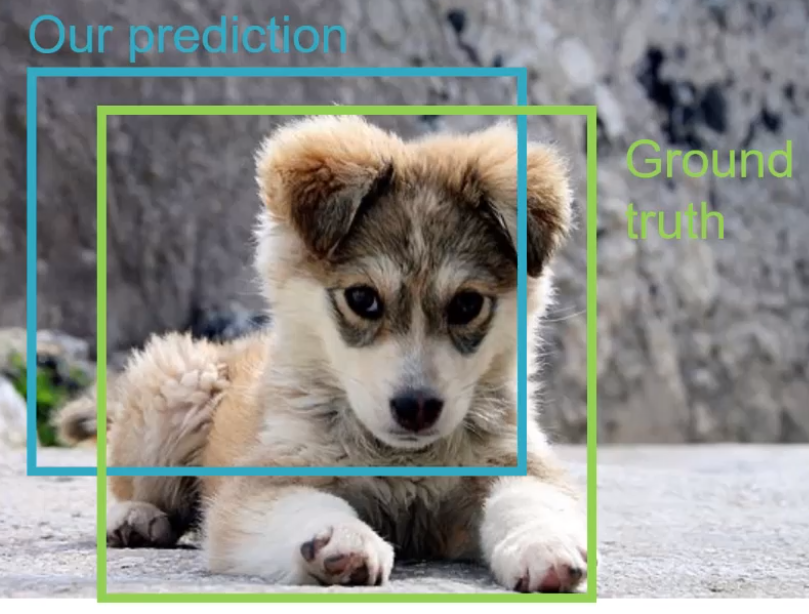
\includegraphics[width=0.5\textwidth]{figures/Intersection_over_union.png}
\caption{Comparing predicted object to the actual object (manually annotated)}
\label{fig:intersection_over_union}
\end{figure} 

\begin{itemize}
	\item There may be many \textbf{oberlapping} boxes.  Solved by \textbf{Non-maximum suppresion} :
		\begin{enumerate}
			\item Select highest scoring box
			\item Eliminate lower IoU scoring boxes by comparing it to every other bounding box. If they are above 0.7.
			\item If overlapping boxes remain, repeat.
		\end{enumerate}
\end{itemize}

\textbf{Mean Average Precision - mAP} \\
For each category compute \textbf{Average Precision} = Area under precision recall curve. \\
The compute the overall mean of the average precessions of all the categories. Gives an overall metric.



% -----------------------------------------------------------------------------------------------------------------------
\newpage
\subsection{CNN: Semantic and instance segmentation}
\subsubsection{Semantic segmentation}
\textbf{Label each pixel with a category, no instances of objects.} 
\begin{figure}[H]
\centering
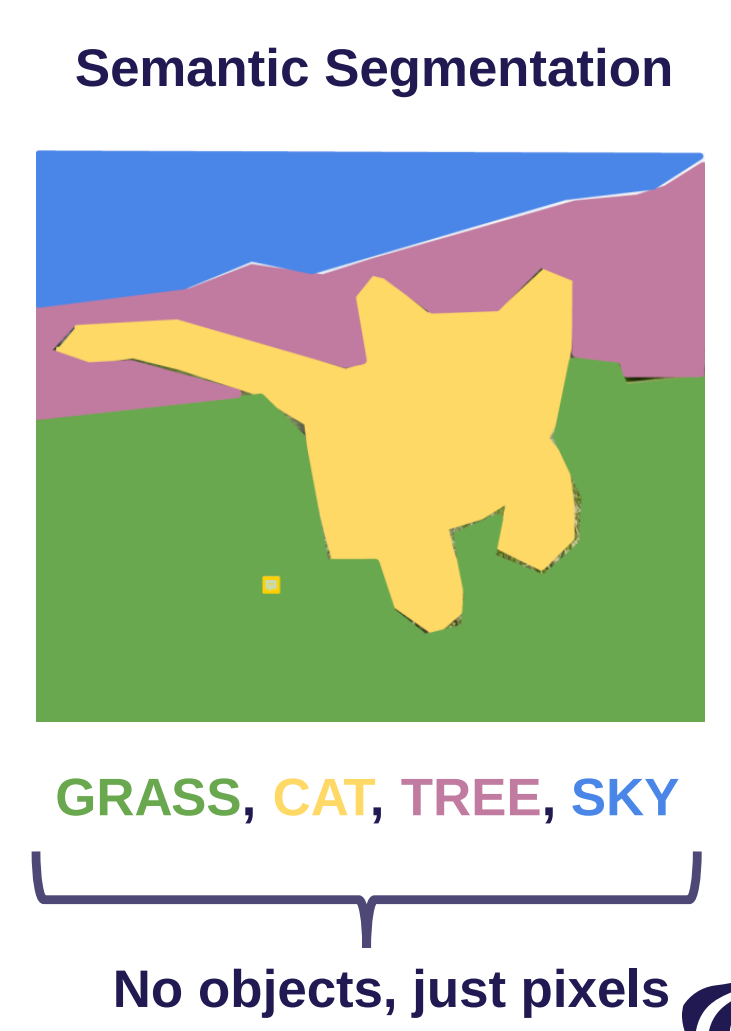
\includegraphics[width=0.4\textwidth]{figures/Semantic_segmentation.png}
\caption{Illustration of semantic segmentation}
\label{fig:semantic_segmentation}
\end{figure} 

Output image is same resolution as input image. $ \rightarrow $ apply 0 padding \\

\subsubsection*{Done with fully convolutional network}
\begin{figure}[H]
\centering
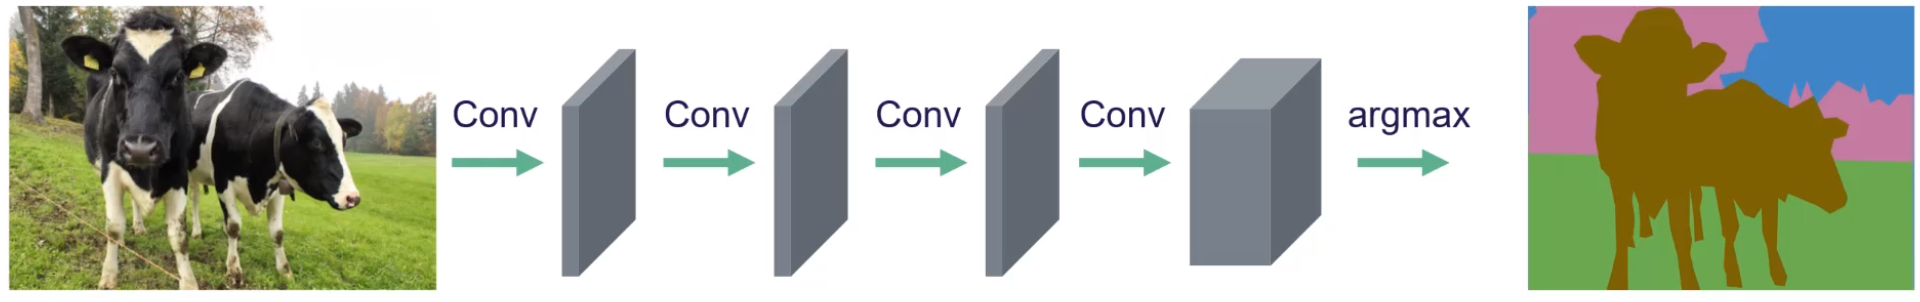
\includegraphics[width=0.9\textwidth]{figures/Fully_convolutional_network_SS.png}
\caption{Fully convolutional network that preserves the image resolution through the network.}
\label{fig:fully_convolutional_network}
\end{figure} 

\textbf{Problems:} 
\begin{itemize}
	\item We have relatively \textbf{small receptive field}. Many sequential convolutions are required to expand receptive field $ \rightarrow $ expensive 
	\item High res images are expensive. 
\end{itemize}

\subsubsection*{Could be solved by reducing image size and expanding it in the end}
Done using \textbf{downsampling (pooling)} and \textbf{upsampling} 

\subsubsection*{Upsampling}
\textbf{Transposed convolution}. Done by introducing padding in the lower resolution input image. Can be \textbf{learned}. \\
Use \textbf{skip connections} to preserve fine-grained textural information.  
\begin{figure}[H]
\centering
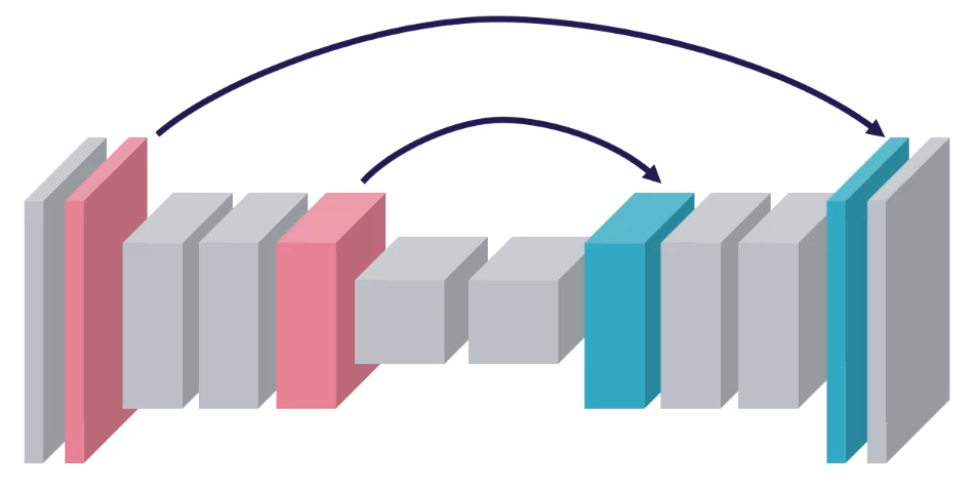
\includegraphics[width=0.6\textwidth]{figures/Downsampling_upsampling.png}
\caption{Illustration of a downscaling and upscaling network with \textbf{skip connections}}
\label{fig:down_up}
\end{figure} 



\textbf{MS-COCO} is a dataset that includes Instance segmentation. Not just single classifications for an image. 


\subsubsection{Instance segmentation}
Decide what object instance a pixel belongs to.

\subsubsection*{Mask R-CNN}
Build on Faster R-CNN

\begin{figure}[H]
\centering
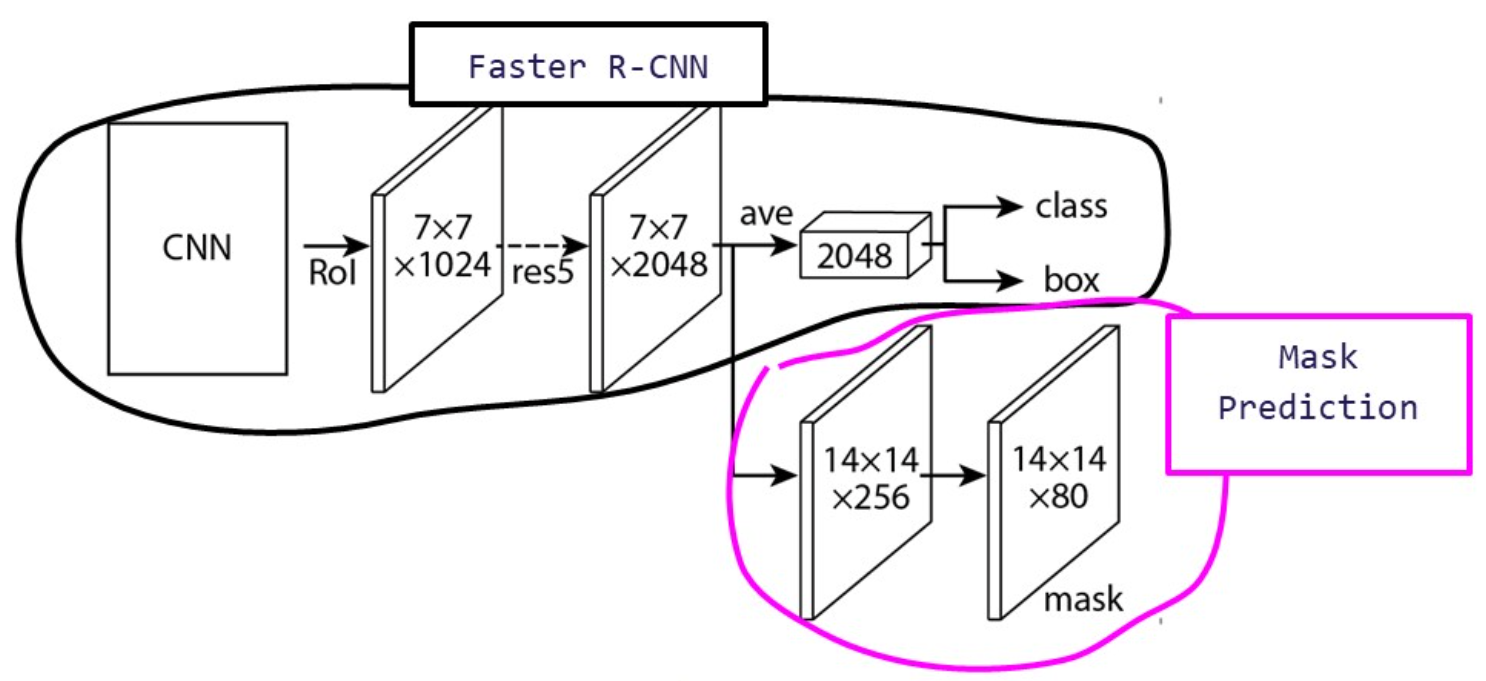
\includegraphics[width=0.8\textwidth]{figures/Mask_RCNN.png}
\caption{Mask R-CNN}
\label{fig:mask_RCNN}
\end{figure} 

\begin{itemize}
	\item Fast R-CNN outputs probability of belonging to class x and the bounding box associated with it. 
	\item The pink part predicts the mask (outline) of the instance. 
\end{itemize}


% -----------------------------------------------------------------------------------------------------------------------
\newpage
\subsection{CNN: Pose estimation}
We estimate the human poses with joints and links, such that they look like a skeleton. 
\begin{figure}[H]
\centering
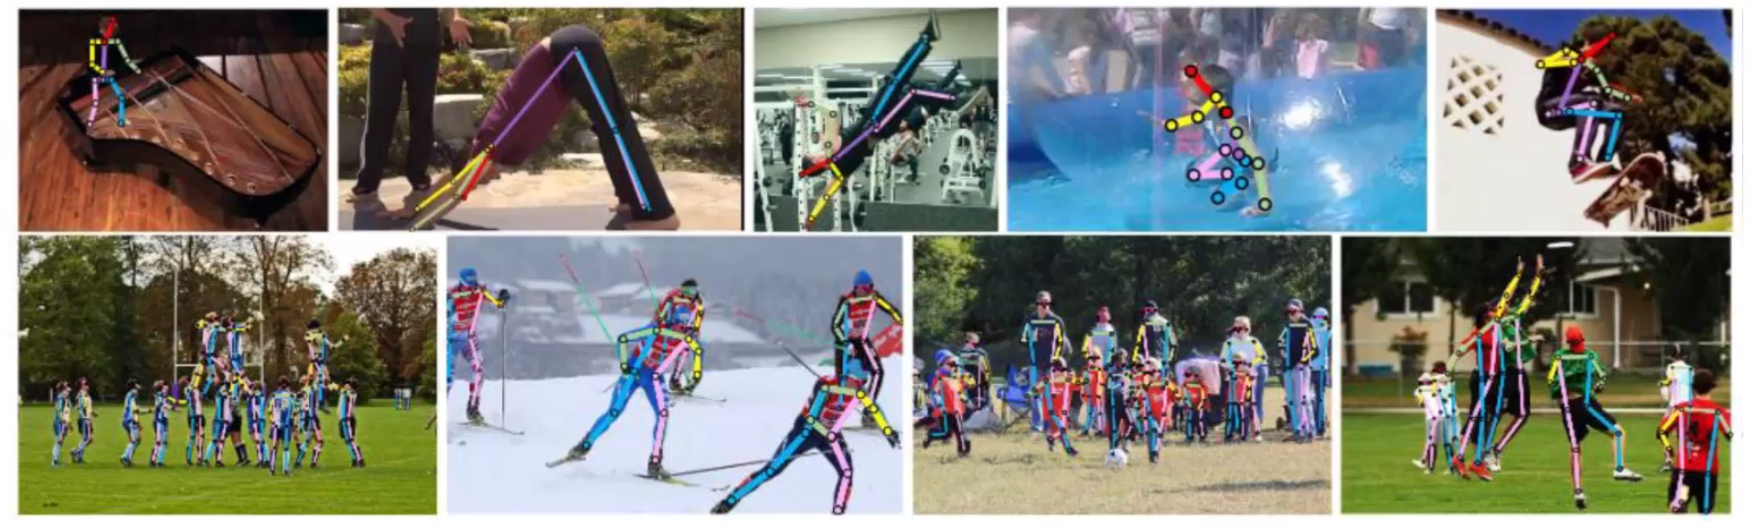
\includegraphics[width=0.99\textwidth]{figures/Human_pose_estimation.png}
\caption{Human pose estimation}
\label{fig:human_pose_estimation}
\end{figure} 

\textbf{Goal: estimate 2D or 3D positions of joints. } 

\textbf{Problems:} 
\begin{itemize}
	\item Many degrees of freedom
	\item Varying clothes / appearance
	\item Self occlusions
\end{itemize}

\textbf{pre-deep learning:} Pictorial structures in 2D. Set relative constraints (springs) between the joints. 

\subsubsection*{2D Pose estimation - DNN}
\begin{itemize}
	\item \textbf{DeepPose:} first DNN method. Based on itteratively refining the position of the joint. The input size changes from iteration to iteration.
		\begin{figure}[H]
		\centering
		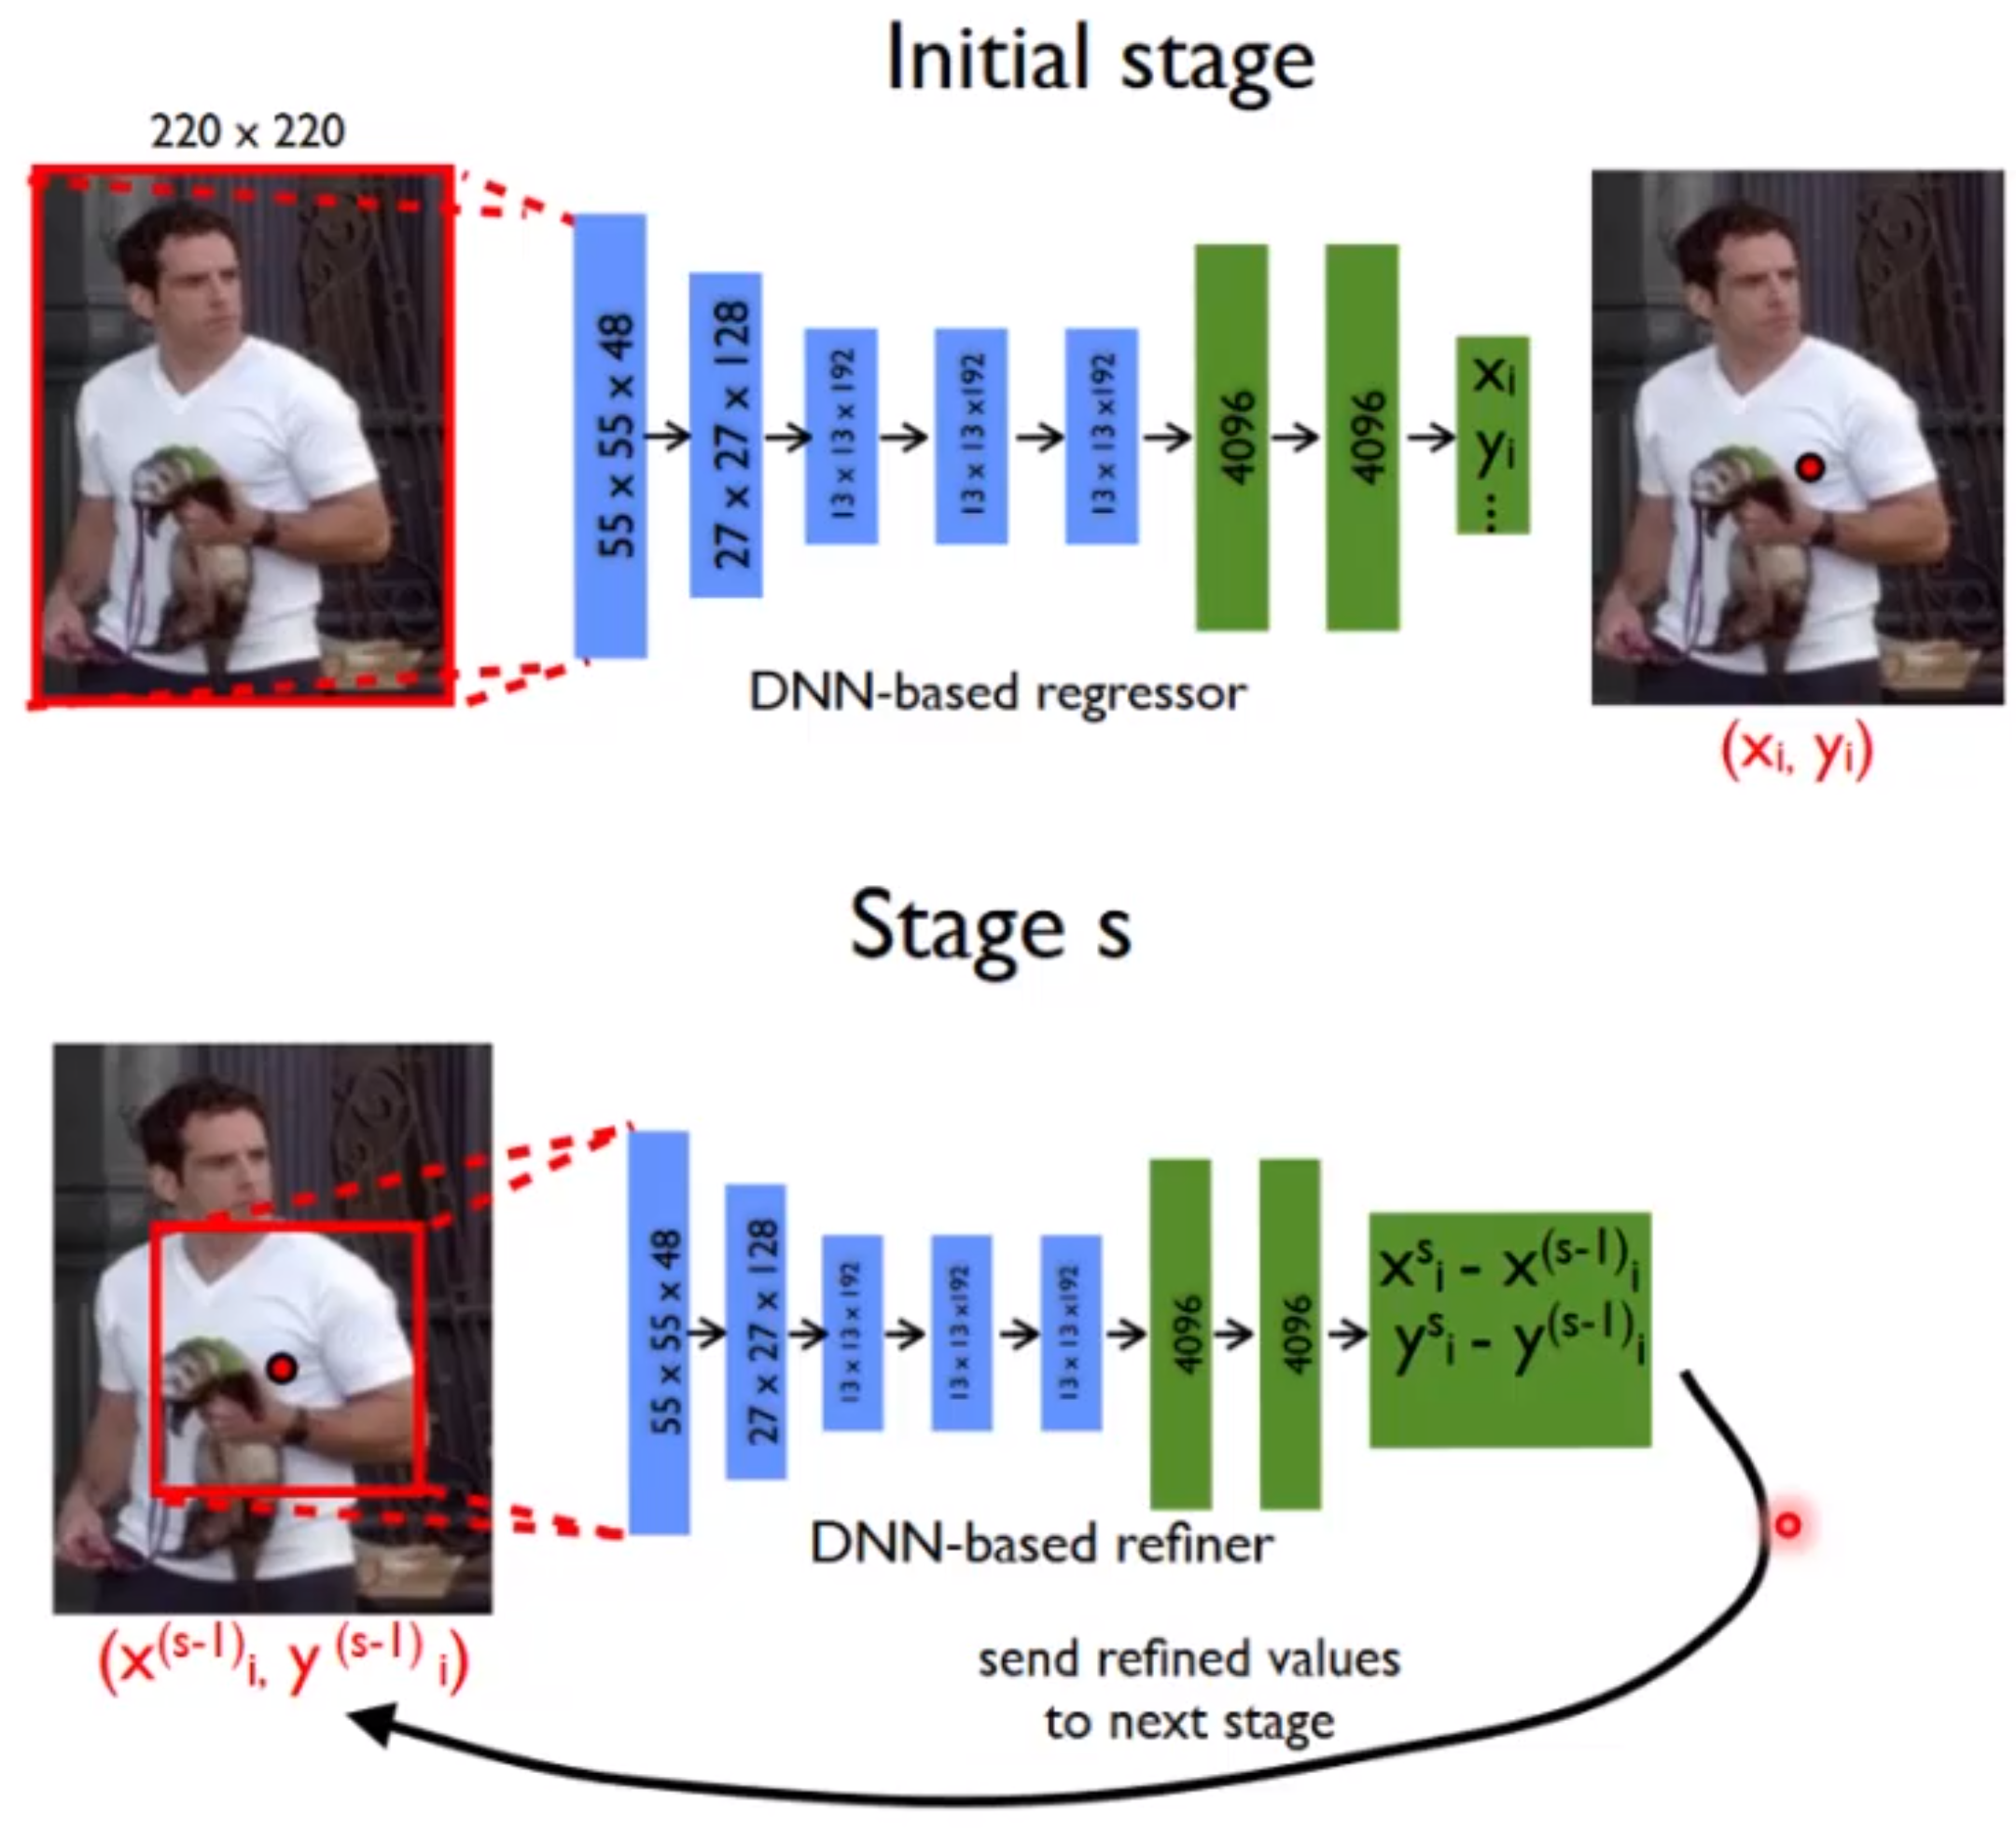
\includegraphics[width=0.6\textwidth]{figures/DeepPose.png}
		\caption{Illustration of the DeepPose algorithm}
		\label{fig:deep_pose_algorithm}
		\end{figure} 
	\item \textbf{Mask R-CNN:} Can be trained to find only a single pixel to illustrate the joints. So instead of masking the entire object, it masks a single pixel. Predict $ k $ joints.  
	\item \textbf{HRNet:} High resolution is maintained through the network.   
		\begin{figure}[H]
		\centering
		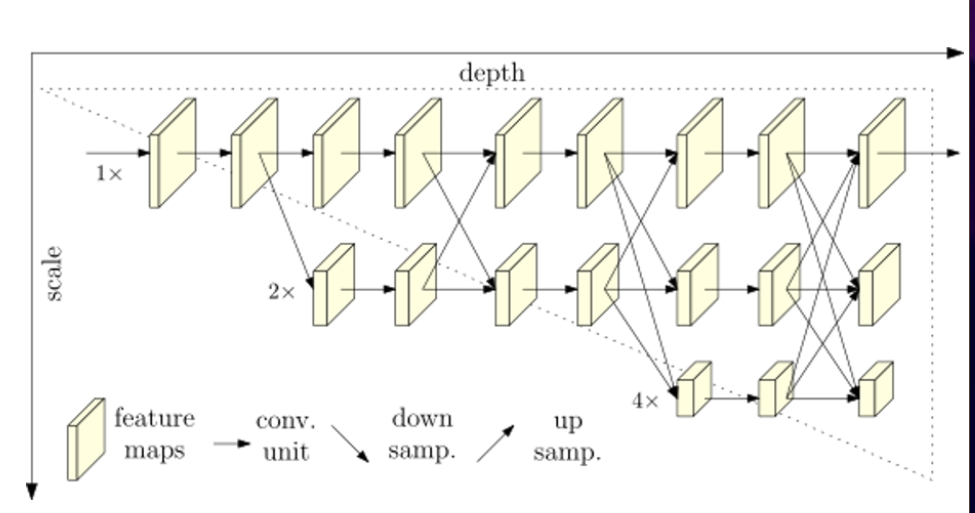
\includegraphics[width=0.8\textwidth]{figures/HRNet.png}
		\caption{HRNet network}
		\label{fig:HRNet}
		\end{figure} 
\end{itemize} 


\subsubsection*{3D Pose estimation}
\textbf{Requires Ground truth} with motion tracking systems. Expensive. \\

You can also input 3D features into the network, e.g. depth camera input or multiview. \\


\textbf{DNN approach} 
\begin{enumerate}
	\item Use a large dataset of 3D poses and take numerous 2D images from arbitrary angles. 
	\item Use the 3D, 2D pairs as training data.
	\item Given a input image, find 2D pose
	\item Find best matching 2D pose from the dataset, and output the corresponding 3D pose.
\end{enumerate}


% -----------------------------------------------------------------------------------------------------------------------
\newpage
\subsection{Point cloud processing}
\begin{itemize}
	\item Set of 3D coordinates
	\item May include additional information like \textbf{Surface normal, color} 
\end{itemize}

You can compute point clouds from e.g. 
\begin{itemize}
	\item Depth from disparity (stereo vision)
	\item Directly measure them from sensors
	\item Can be computed from RGB-D using intrinsic and extrinsic camera paratmers. 
		\begin{equation}
		\begin{bmatrix}
		X \\
		Y \\
		Z
		\end{bmatrix} = d \begin{bmatrix}
		\frac{u - u_0}{f_x}  \\
		\frac{v-v_0}{f_y} \\
		1
		\end{bmatrix} 
		\end{equation}
		where $ u,v $ are the image coordinates with depth $ d $, and $ u_0,v_0 $ are the optical center. $ f_x, f_y $ being focal length in pixels and  $ X,Y,Z $ being 3D camera coordinates.

\end{itemize}

\textbf{PCL: Point Cloud Library} \\
Each of these methods reside in PCL

\subsubsection*{Pass through filter}
Filter the pointcloud \textbf{based on position}. 
Define the positional threshold you want to keep, and then everything else is discarded. 

\subsubsection*{Outlier removal}
Can be done with \textbf{StatisticalOutlierremoval}.

\begin{enumerate}
	\item Measures distance from each point to its 50 closest neighbors
	\item Computes the mean and standard deviations from these distances
	\item if a point is over 1 std. away from the point, then it is discarded. 
\end{enumerate}

\subsubsection*{Clustering}
By specifying a max distance from a point that a point must be to be within a cluster, we can define clusters. \\
Note you can specify min- and max cluster size. 



\subsubsection*{RANSAC}
\begin{enumerate}
	\item Randomly sample x points from the pointcloud.
	\item Fit a plane to the points.
	\item Choose inlier distance, and let the model with most inliers win. 
\end{enumerate}

% -----------------------------------------------------------------------------------------------------------------------
\newpage
\subsection{Deep learning for point clouds}
Challenges of using DL for pointclouds
\begin{enumerate}
	\item Images are fixed size with good knowledge of what is to the left and right of a pixel. Pointclouds are not like this.
	\item Can vary in size. 
	\item Unordered list of points. $ \rightarrow $ Unclear neighborhood. 
\end{enumerate}

\subsubsection*{PointNet}
\textbf{Solves the unordered problem} by using a symmetric function (output is the same regardless of input).


This is done by taking a fixed number of points (1024), and running them through \textbf{individual 1D CNN's} and extracts a 1024 dimensional featuremap from this. From here we do max pooling to extract the best feature, and then run it through a Deep Neural network to resolve a label. 
\begin{figure}[H]
\centering
\includegraphics[width=0.99\textwidth]{figures/PointNet.png}
\caption{PointNet}
\label{fig:pointNet}
\end{figure} 




\subsubsection*{Graph Neural Networks}
Resolves all problems: 
\begin{itemize}
	\item Permutation invariance
	\item Cardinality invariance
	\item Neighbourhood features. 
\end{itemize}

The Dynamic Graph CNN computes a neighbourhood for each pixel, and the uses that neighborhood to compute the next featureset through edge convolutions. As more layers are computed, the features becomes enriched with neighborhood information of larger neighborhoods, and become more semanticly apparent. 
\begin{figure}[H]
\centering
\includegraphics[width=0.99\textwidth]{figures/GNN.png}
\caption{Graph Neural Network - Dynamic graph CNN for learning on point clouds}
\label{fig:GNN}
\end{figure} 

% -----------------------------------------------------------------------------------------------------------------------
\newpage
\centering
\section{Mini project}
\raggedright
\newpage
\subsection{Miniproject}

\begin{figure}[H]
\centering
\includegraphics[width=0.99\textwidth]{figures/Miniproject_results.png}
\caption{Miniproject results}
\label{fig:miniproject_results}
\end{figure} 

\begin{figure}[H]
\centering
\includegraphics[width=0.6\textwidth]{figures/RANSAC_miniproject_visualization.png}
\caption{Ransac visualization}
\label{fig:ransac_mini_viz}
\end{figure} 

\textbf{Camera:} 
Intel realsense D435. Has an IR projector and IR 2 sensors. Using camera intrinsics to aquisite the image.
RGB image is $ 1920 \times 1080 $, and Depth is $ 1280 \times 720 $
UV mapping takes the RGB image and maps it to the depth map, such that it has the same resolution. 
We return the Depth image, the color image, and the pointcloud. 

\textbf{HSV:} 
\begin{enumerate}
	\item $ 45 < H < 65 $
	\item $ 35 < H < 255 $
	\item $ 35 < H < 255 $
\end{enumerate}

we set all other verticies to 0,0,0

By using the UV map, we can for each vertex in the pointcloud find the corresponding pixel in the RGB image, and then use the HVS colors on that image to determine if it is green or not. 


\subsubsection*{RANSAC}
From the 3 selected verticies, we generate two vectors and from those, the surface normal vector. 

\subsubsection{Tips}
\begin{itemize}
	\item Use the colors as dimensions in the featurevector in RANSAC
	\item Use Kalman filter to track the plane
	\item Use the previous number of inliers to use as a threshold for exiting the current itteration. $ \rightarrow $ No need to find further planes if we found a plane with similar number of inliers as the previous best inlier. 
\end{itemize}




\end{document}
